\documentclass[12pt, a4paper]{report}

% --- Packages ---
\usepackage[margin=1in]{geometry}
\usepackage{graphicx}
\usepackage[hidelinks]{hyperref}
\usepackage{tikz}
\usetikzlibrary{shapes, arrows.meta, positioning, calc}
\usepackage{setspace}
\usepackage{titlesec}
\usepackage[numbers]{natbib}
\usepackage{fancyhdr}
\usepackage{etoolbox}

% --- Document Settings ---
\onehalfspacing
\setlength{\parskip}{1em}
\setlength{\parindent}{0pt}

% --- Chapter Formatting ---
\titleformat{\chapter}[display]
  {\normalfont\huge\bfseries}{\chaptertitlename\ \thechapter}{20pt}{\Huge}
\titlespacing*{\chapter}{0pt}{-20pt}{20pt}

% --- PDF Metadata ---
\hypersetup{
    pdftitle={Intelligent Compliance Management System (ICMS)},
    pdfauthor={Muhammad Ali Bukhari, Hammad Chaghtai},
    pdfsubject={Final Year Project Thesis},
    pdfkeywords={GRC, SIEM, Wazuh, Compliance, Automation}
}

\begin{document}

% =========================================================
% TITLE PAGE
% =========================================================
\begin{titlepage}
    \centering
    \vspace*{1cm}
    
    
\includegraphics[width=0.3\textwidth]{bui_logo.jpg}\\[1.5cm]
    
    {\Huge \textbf{Intelligent Compliance Management System (ICMS)}}\\[1.5cm]
    
    {\Large \textbf{Muhammad Ali Bukhari (01-135222-096)}}\\[0.3cm]
    {\Large \textbf{Hammad Chaghtai (01-135222-014)}}\\[1.5cm]
    
    {\large \textbf{Supervisor: Dr. Faisal Bashir}}\\[2cm]
    
    {\large \textbf{Bachelor of Science in Information Technology}}\\[1cm]
    
    {\large \textbf{Department of Computer Science}}\\[0.2cm]
    {\large \textbf{Bahria University, Islamabad}}\\[1.5cm]
    
    {\large \textbf{April 2026}}
    
    \vfill
\end{titlepage}

% =========================================================
% APPROVAL CERTIFICATE
% =========================================================
\newpage
\pagenumbering{roman}
\section*{Certificate of Approval}
\addcontentsline{toc}{section}{Certificate of Approval}
\vspace{1cm}

We accept the work contained in the report titled \textbf{``Intelligent Compliance Management System (ICMS)''}, written by \textbf{Muhammad Ali Bukhari} and \textbf{Hammad Chaghtai} as a confirmation to the required standard for the partial fulfillment of the degree of Bachelor of Science in Information Technology.

\vspace{2cm}

\begin{flushleft}
    \textbf{Approved by:}
    \vspace{1.5cm}
    
    \rule{8cm}{0.4pt}\\
    \textbf{Supervisor: Dr. Faisal Bashir}\\
    (Department of Computer Science)
    
    \vspace{1.5cm}
    
    \rule{8cm}{0.4pt}\\
    \textbf{Internal Examiner: Name of the Internal Examiner}\\
    (Title/Designation)
    
    \vspace{1.5cm}
    
    \rule{8cm}{0.4pt}\\
    \textbf{External Examiner: Name of the External Examiner}\\
    (Title/Designation)
    
    \vspace{1.5cm}
    
    \rule{8cm}{0.4pt}\\
    \textbf{Head of Department: Name of the HOD}\\
    (Department of Computer Science)
\end{flushleft}

% =========================================================
% ABSTRACT
% =========================================================
\newpage
\section*{Abstract}
\addcontentsline{toc}{section}{Abstract}

Manual security auditing in enterprise environments fails to address rapid configuration drift or ephemeral workloads effectively. This thesis presents the Intelligent Compliance Management System (ICMS), a full-stack platform designed to automate Governance, Risk, and Compliance (GRC) workflows through direct Security Information and Event Management (SIEM) integration. The system utilizes a specialized client to ingest raw telemetry from Wazuh, mapping technical events to specific control requirements within the ISO 27001:2022 and SOC 2 Type II frameworks. To manage the performance demands of real-time monitoring, the architecture eliminates the N+1 query bottleneck by implementing set-based ORM aggregation and SQL FILTER clauses. This optimization converts linear retrieval patterns into constant-time database operations, allowing the dashboard to aggregate millions of telemetry rows without significant latency. When telemetry sources provide contradictory states, the system applies a Worst-Case Priority algorithm to ensure a pessimistic, secure resolution of compliance statuses. Infrastructure security follows a defense-in-depth model, utilizing a containerized topology that isolates the PostgreSQL data tier and Redis message broker within a private Docker bridge network. This isolation prevents direct host-port exposure and restricts lateral movement during a potential breach. Identity management relies on stateless JSON Web Tokens (JWT) with rotation policies and Time-Based One-Time Passwords (TOTP) to maintain a zero-trust baseline. The resulting framework replaces periodic, manual evidence collection with a continuous, data-driven assessment model that provides deterministic validation of an organization's security posture.

% =========================================================
% ACKNOWLEDGMENTS
% =========================================================
\newpage
\section*{Acknowledgments}
\addcontentsline{toc}{section}{Acknowledgments}

In the name of Allah, the Most Gracious, the Most Merciful. All praise is due to Allah, the Almighty, for granting the strength and guidance required to complete this work.

I express my deepest gratitude to my supervisor, Dr. Faisal Bashir, for his mentorship, technical expertise, and continuous encouragement throughout the development of this project. His insights into systems architecture and cybersecurity were fundamental to the successful execution of this thesis.

I am also thankful to the Department of Computer Science at Bahria University for providing the academic environment and resources necessary for our research. Finally, I would like to thank my family and peers for their unwavering support and patience during this intensive process.

\vspace{1cm}
\begin{flushright}
    \textbf{Muhammad Ali Bukhari}\\
    \textbf{Hammad Chaghtai}
\end{flushright}

% =========================================================
% TABLE OF CONTENTS / LISTS
% =========================================================
\newpage
\tableofcontents

\newpage
\listoffigures

\newpage
\listoftables

% =========================================================
% CHAPTERS
% =========================================================
\newpage
\pagenumbering{arabic}

\chapter{Introduction}

\section{Background of Enterprise Compliance}

Historical security auditing methodologies rely on manual evidence collection and point-in-time assessments. Organizations traditionally compile spreadsheets and static configuration snapshots to satisfy periodic regulatory requirements. This approach creates significant temporal blind spots, as the security posture remains unverified between audit cycles. Configuration drift often occurs within hours of a successful audit, leaving the infrastructure vulnerable to exploitation while maintaining a formal status of compliance.

The cybersecurity industry addresses these vulnerabilities by transitioning toward Continuous Controls Monitoring (CCM). This paradigm shift replaces manual sampling with automated, real-time validation of security controls. CCM platforms integrate directly with the technical environment to evaluate configurations, access logs, and system integrity continuously. This automation ensures that compliance reflects the actual, current state of the environment rather than a historical record.

Modern regulatory mandates codify the requirement for continuous visibility. NIST Special Publication 800-53 Revision 5 emphasizes the transition from static control assessments to ongoing monitoring to validate system integrity \cite{nist80053_2020}. Similarly, the ISO/IEC 27001:2022 standard requires organizations to establish an Information Security Management System (ISMS) that identifies and treats risks through continuous evaluation \cite{iso27001_2022}. These frameworks necessitate the adoption of technological solutions capable of mapping raw system data to high-level compliance objectives.

The integration of Security Information and Event Management (SIEM) systems provides the data foundation for this automated GRC architecture. SIEM engines ingest raw telemetry from across the enterprise, translating low-level system events into verifiable compliance states. By establishing deterministic baselines, organizations move from reactive, audit-driven reporting to proactive, data-driven security management. This thesis evaluates the implementation of an intelligent system that bridge the gap between technical SIEM telemetry and regulatory control satisfaction.

\section{Problem Statement}

Translating massive volumes of low-level endpoint telemetry into high-level regulatory frameworks presents a significant operational hurdle. SIEM platforms generate thousands of technical alerts, such as SSH authentication failures or unauthorized file modifications, which require immediate correlation against ISO 27001 or SOC 2 control matrices. Manual correlation processes introduce dangerous delays between event detection and compliance validation, creating a window of risk where system vulnerabilities remain unaddressed. Concurrent telemetry sources often produce contradictory states, requiring deterministic resolution mechanisms that existing manual workflows cannot provide.

Calculating real-time compliance metrics across distributed fleets exposes severe data aggregation failures in traditional GRC platforms. Standard relational database implementations often suffer from the N+1 query problem, where the application executes sequential retrieval loops for every individual security control. This architectural flaw imposes a linear $O(N)$ algorithmic complexity on data retrieval, causing geometric performance decay as the number of monitored agents increases \cite{planetscale_n1}. The resulting latency prevents organizations from achieving a truly continuous monitoring state, as dashboard rendering times exceed the threshold for effective operational visibility.

Legacy GRC interfaces fail to account for the cognitive limitations of security analysts. Rigid, HTML table-heavy dashboards and unoptimized color schemes maximize extraneous cognitive load, leading to rapid desensitization known as alert fatigue. Chronic overstimulation from noisy, unfiltered telemetry streams depletes essential neurotransmitters, causing operators to ignore or misclassify high-severity threats \cite{mit_alert_fatigue}. This Human-Computer Interaction (HCI) shortcoming transforms security tools into sources of distraction, ultimately degrading incident response times and increasing organizational risk.

\section{Project Objectives}

The development of the Intelligent Compliance Management System (ICMS) focuses on four primary engineering objectives designed to resolve the identified technical and operational gaps:

\begin{itemize}
    \item Automate the ingestion and mapping of Wazuh SIEM telemetry to ISO 27001 and SOC 2 controls, utilizing a deterministic Worst-Case Priority state-mutation algorithm to resolve conflicting evaluations.
    \item Eliminate the N+1 database querying bottleneck by engineering $O(1)$ set-based aggregations through the Django ORM, specifically utilizing \texttt{.annotate()} and conditional SQL filtering to ensure dashboard latency remains below 200 milliseconds.
    \item Enforce strict infrastructure and session security through a Dockerized virtual bridge network that isolates the PostgreSQL data tier, combined with custom Django REST Framework Role-Based Access Control and stateless JWT rotation.
    \item Mitigate analyst alert fatigue by architecting a Cyber-SaaS frontend that replaces rigid HTML tables with Flexbox layouts and utilizes semantic soft-scaling to improve data parsing speeds.
\end{itemize}

\section{Project Scope}

The Intelligent Compliance Management System (ICMS) strictly operates within the boundaries of the ISO/IEC 27001:2022 and SOC 2 Type II compliance frameworks. The platform scope encompasses the ingestion and mapping of endpoint security telemetry specifically from the Wazuh Manager's Security Configuration Assessment (SCA) module. By utilizing the Wazuh REST API, the system retrieves individual check results from active agents and correlates them to the identified governance controls. This data-driven mapping ensures that the compliance state represents an actual reflection of the technical environment's configuration.

The implementation boundary is restricted to a containerized Docker ecosystem designed for secure, isolated operation. This environment utilizes a private virtual bridge network to facilitate communication between the PostgreSQL database, Redis message broker, Celery workers, and the Django-React application stack. This architectural scope ensures that the data persistence tier remains inaccessible to external networks, maintaining a secure baseline for the storage of sensitive compliance telemetry and organizational policies.

To maintain the focus on Governance, Risk, and Compliance (GRC) monitoring, several operational domains remain outside the project scope. The system does not perform active Incident Response (IR) actions, such as isolating compromised endpoints or terminating malicious processes. The platform does not conduct network packet sniffing or automated remediation of configuration drift. While the system evaluates and reports on the compliance state, it does not mutate endpoint configurations; all infrastructure remediation remains the responsibility of dedicated IT operations teams.

\section{Proposed Solution Overview}

The Intelligent Compliance Management System (ICMS) adopts a defense-in-depth, containerized architecture designed to maintain strict logical separation between processing tiers. The platform utilizes the Django REST Framework for backend orchestration, while a React Single Page Application (SPA) provides a dynamic, Cyber-SaaS user interface. This separation ensures that the frontend remains stateless, relying on cryptographically signed JSON Web Tokens (JWT) for secure API communication.

Within the containerized ecosystem, the system isolates critical data persistence and messaging layers. The PostgreSQL database and Redis message broker operate on a private virtual bridge network, restricting access to the internal backend and Celery worker services. This topology prevents direct external exposure of compliance telemetry and session data. The Celery workers and scheduler manage periodic Wazuh SIEM synchronization, while the Django API serves as the central gateway for framework mapping and report generation.

\begin{figure}[htbp]
    \centering
    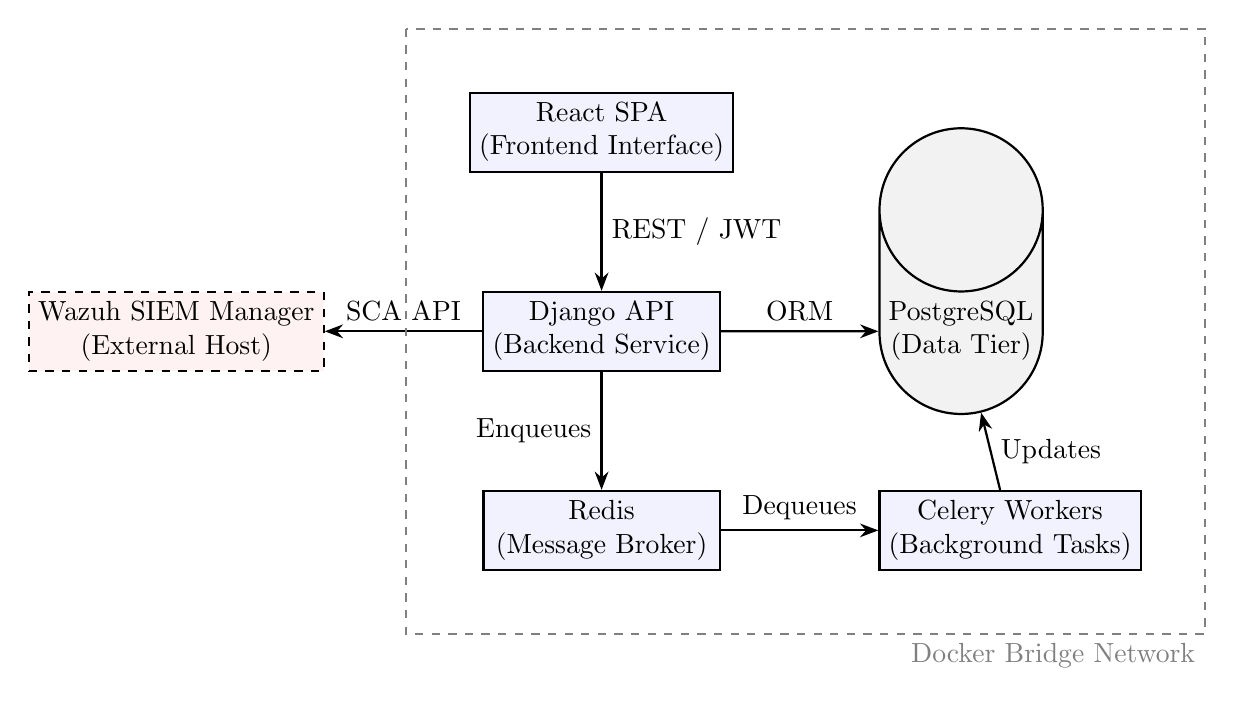
\begin{tikzpicture}[
        node distance=1.5cm and 2cm,
        service/.style={rectangle, draw, minimum width=3cm, minimum height=1cm, align=center, fill=blue!5, thick},
        database/.style={cylinder, draw, shape border rotate=90, minimum width=2cm, minimum height=1.5cm, align=center, fill=gray!10, thick},
        external/.style={rectangle, draw, dashed, minimum width=3cm, minimum height=1cm, align=center, fill=red!5, thick},
        arrow/.style={-Stealth, thick}
    ]
        % Nodes
        \node[external] (wazuh) {Wazuh SIEM Manager\\(External Host)};
        \node[service, right=of wazuh] (backend) {Django API\\(Backend Service)};
        \node[service, above=of backend] (frontend) {React SPA\\(Frontend Interface)};
        \node[database, right=of backend] (db) {PostgreSQL\\(Data Tier)};
        \node[service, below=of backend] (redis) {Redis\\(Message Broker)};
        \node[service, right=of redis] (celery) {Celery Workers\\(Background Tasks)};

        % Paths
        \draw[arrow] (frontend) -- (backend) node[midway, right] {REST / JWT};
        \draw[arrow] (backend) -- (wazuh) node[midway, above] {SCA API};
        \draw[arrow] (backend) -- (db) node[midway, above] {ORM};
        \draw[arrow] (backend) -- (redis) node[midway, left] {Enqueues};
        \draw[arrow] (redis) -- (celery) node[midway, above] {Dequeues};
        \draw[arrow] (celery) -- (db) node[midway, right] {Updates};

        % Container Boundary (Visual Representation)
        \draw[gray, dashed, thick] ($(frontend.north west)+(-0.8,0.8)$ ) rectangle ($(celery.south east)+(0.8,-0.8)$);
        \node[gray, anchor=north east] at ($(celery.south east)+(0.8,-0.8)$) {Docker Bridge Network};

    \end{tikzpicture}
    \caption{High-Level Architecture of the Containerized ICMS Platform}
    \label{fig:high_level_architecture}
\end{figure}

\section{Thesis Organization}

This thesis consists of seven chapters that detail the research, design, and implementation of the Intelligent Compliance Management System (ICMS). Chapter 2 evaluates existing literature regarding Governance, Risk, and Compliance (GRC) frameworks and Security Information and Event Management (SIEM) integration. Chapter 3 defines the functional and non-functional requirements of the platform while establishing the high-level system architecture. Chapter 4 provides the detailed system design, incorporating Unified Modeling Language (UML) diagrams to represent the logical and physical data flows. Chapter 5 focuses on the implementation phase, detailing the backend algorithms and containerized orchestration used to achieve continuous monitoring. Chapter 6 outlines the system testing protocols and evaluates the platform's performance against defined accuracy and latency metrics. Chapter 7 concludes the research by summarizing the project's contributions and proposing directions for future work.

\chapter{Literature Review}

\section{Comprehensive Literature Review}

\subsection{Evolution of Governance, Risk, and Compliance (GRC) Platforms}
Historical security auditing relied on point-in-time assessments, leaving temporal blind spots between evaluation periods. Organizations managed Governance, Risk, and Compliance (GRC) through manual evidence collection, rendering the compliance state obsolete following an assessment. Regulatory frameworks require a transition toward continuous controls monitoring architectures. Standards including NIST Special Publication 800-53 Revision 5 and ISO/IEC 27001:2022 mandate ongoing monitoring to validate control implementation \cite{nist80053_2020, iso27001_2022}. The Federal Information Security Modernization Act (FISMA) and the Federal Risk and Authorization Management Program (FedRAMP) require agencies to automate the tracking of systemic anomalies \cite{fisma_2014}. The transition to SIEM-driven compliance introduces operational advantages. Centralized log management supports audit accountability by preserving data confidentiality, integrity, and availability \cite{nist80092_2006}. Automated analysis establishes operational baselines, facilitating forensic investigations during security incidents. Security administrators configure SIEM agents to track software inventories, hardware configurations, and system health telemetry, feeding this data into the GRC database. Continuous validation replaces reactive audits with a data-driven security posture. By evaluating log streams against established baselines, organizations ensure evidence generation becomes a byproduct of daily security operations.

\subsection{Security Information and Event Management (SIEM) Integrations}
The integration of Security Information and Event Management (SIEM) systems alters the GRC methodology. SIEM platforms act as telemetry ingestion engines, replacing manual log retrieval with automated data correlation. NIST SP 800-53 defines control families, notably Audit and Accountability (AU) and System and Information Integrity (SI), which require automated tracking to satisfy continuous validation requirements \cite{nist80053_2020}. Automating these controls involves mapping endpoint telemetry directly to regulatory requirements. Platforms like Wazuh, an open-source SIEM and Extended Detection and Response (XDR) solution, facilitate this translation by supplying event aggregation logic that maps compliance events against NIST and ISO matrices \cite{wazuh_doc}. Automated compliance mapping bridges the semantic gap between technical events and business risk. When a user modifies a protected configuration file, File Integrity Monitoring (FIM) sensors generate an event log. The SIEM correlates this event against framework matrices, flagging the action as a violation of ISO 27001 Annex A.8.9 (Configuration Management) or NIST SP 800-53 control CM-6 \cite{nist800128_2011}. Analysts monitor deviations via dashboards that aggregate alert volumes, isolating non-compliant agents for remediation. The Wazuh Security Configuration Assessment (SCA) module provides the deterministic validation required to satisfy these governance frameworks by evaluating configuration states against security benchmarks.

\subsection{Performance Bottlenecks in Telemetry Aggregation}
Calculating compliance metrics across distributed fleets exposes data aggregation limitations in traditional GRC platforms. Standard relational database implementations suffer from the N+1 query problem, where the application executes sequential retrieval loops for individual security controls. This architectural flaw imposes a linear $O(N)$ algorithmic complexity on data retrieval, causing geometric performance decay as monitored agents increase \cite{planetscale_n1}. The resulting latency prevents organizations from achieving continuous monitoring, because dashboard rendering times exceed thresholds for operational visibility. The overhead associated with Object-Relational Mapping (ORM) frameworks extends beyond query volume. Application-level data processing, where the system retrieves full object graphs before filtering or aggregating in the Python memory space, creates memory bandwidth bottlenecks. This pattern forces the application server to instantiate transient objects, triggering garbage collection cycles that block the execution of compliance logic. In environments where SIEM agents transmit telemetry continuously, the cumulative impact of these $O(N)$ operations leads to a loss of operational visibility.

Optimizing relational data access requires transitioning from sequential $O(N)$ looping to $O(1)$ set-based aggregations. Set-based modeling formalizes relational dynamics, demonstrating that task-informed database representations retain relevant signals more efficiently than application-level iteration \cite{kuraj_microservices_2024}. Developers optimize ORM queries by utilizing eager loading mechanisms that translate application logic into SQL JOIN clauses. Fetching related entities in a single query allows the database engine's internal query optimizer to utilize B-Tree indices efficiently, reducing total execution time and minimizing context switching between the application runtime and the database server. Set-based database aggregations shift the mathematical workload to the relational engine. Using query projection techniques, the system instructs the database to compute sums, averages, and conditional compliance counts internally. This methodology reduces data transfer across the network wire from megabytes of row data to primitive integer values. By utilizing conditional aggregation functions, where the engine evaluates compliance criteria during the initial table scan, the platform achieves a deterministic $O(1)$ response time. Implementing these optimizations ensures dashboard rendering remains responsive as the organizational asset inventory scales. The architectural decision to prioritize database-side computation over application-side iteration reflects the principle of pushing logic closer to the data. This approach ensures the GRC platform can process telemetry logs without exhausting the system's computational resources.

\subsection{Modern Access Control Paradigms}
Securing the compliance data layer against unauthorized extraction requires Identity and Access Management (IAM) protocols. Role-Based Access Control (RBAC) provides the foundation for authorization within distributed systems. RBAC methodologies control access to system resources based on roles assigned to a user, rather than assigning explicit permissions directly to the user identity \cite{nelson_stateless_2024}. Authentication in distributed microservices relies on stateless session security, primarily implemented via JSON Web Tokens (JWT). The authorization server cryptographically signs the JWT using asymmetric encryption algorithms, preventing payload tampering and allowing local verification without initiating a database lookup. Authorization in the ICMS platform relies on an enforcement layer that integrates Zero Trust principles into the API routing logic. Rather than assuming internal network trust, the system evaluates the identity context of every inbound request. Custom permission classes intercept traffic at the view layer, executing Boolean logic to verify the requester possesses the RBAC attributes required for the target resource. This enforcement remains decoupled from the business logic, ensuring a consistent security boundary across the microservice ecosystem.

The security lifecycle of stateless JSON Web Tokens (JWT) incorporates rotation policies to mitigate risks inherent in long-lived credentials. Traditional session IDs require database lookups to verify validity; JWTs carry cryptographically signed claims that allow microservices to authenticate users locally. To prevent session hijacking via intercepted tokens, the platform implements a refresh token rotation scheme. When the client requests a new access credential, the server invalidates the previous refresh token and issues a new pair, ensuring compromised credentials have limited utility. The architecture incorporates Time-Based One-Time Passwords (TOTP) as a secondary authentication factor. TOTP algorithms rely on a high-entropy, shared cryptographic secret established between the server and the client's authenticator application. Both entities use the current Unix timestamp, divided by a predetermined time interval, as the moving factor in a Keyed-Hash Message Authentication Code (HMAC-SHA1) function \cite{rfc6238}. Because the resulting 6-digit numeric code mutates deterministically every 30 seconds, intercepted credentials become mathematically useless. Secondary authentication factors establish an additional defensive layer that remains resilient against replay attacks. Client-side interceptors monitor for specific HTTP response states; when the server returns a forbidden status due to a missing or invalid TOTP challenge, the application redirects the user to a step-up authentication view, preventing unauthorized access. This session lifecycle ensures the compliance data remains inaccessible to compromised endpoints.

\subsection{Containerization and Defense-in-Depth Topology}
Enterprise architecture increasingly transitions from monolithic software design toward microservices and containerized deployments. Monolithic systems couple application logic, user interfaces, and database drivers into a single deployment artifact, where a failure in one component frequently cascades across the runtime environment. Containerization technologies, specifically Docker, provide the standardized runtime environment for these distributed microservices, ensuring deterministic scalability and bounded contexts through Linux kernel namespaces and control groups. Deploying the ICMS components via isolated Docker virtual bridge networks establishes a defense-in-depth topology. The architecture physically separates the public-facing API gateway layers from the private persistent storage layers, such as PostgreSQL and Redis. By binding these data tiers to internal, non-routable Docker bridge networks, the system remains inaccessible to external network scans. This isolation ensures actors cannot establish direct TCP connections with the database, forcing data interactions through the authenticated business-logic layer. Adherence to external hardening standards, such as NIST SP 800-190 and the CIS Docker Benchmark, further neutralizes execution environment vulnerabilities \cite{nist800190_2017, cis_docker_2020}.

\subsection{Cognitive Load and HCI in Security Dashboards}
Security Operations Centers process large volumes of diagnostic data daily, frequently triggering alert fatigue. Legacy GRC platforms present analysts with unfiltered data in dense HTML tables, leading to sensory overload and an increase in diagnostic errors. High cognitive load correlates with delayed incident response times and operator burnout \cite{mit_hci_security_2022}. Mitigating cognitive strain requires the application of User Interface (UI) design principles based on human-computer interaction studies. Modern browser rendering engines deprecate structural tables for layout purposes in favor of CSS Flexbox and Grid modules, which allow child components to wrap and scale fluidly based on viewport dimensions \cite{mdn_flexbox}. The ICMS platform utilizes modular card components and semantic color scaling, such as bold red for critical exploits and minimal grayscale for benign logs, to guide the analyst's focus toward critical threats. Leveraging elevation through depth illusions distinguishes interactive components from static background data, structuring telemetry into a decision-support matrix.

\section{Analysis of Existing Systems}

\subsection{Manual Spreadsheet Auditing}
Evaluating the baseline of traditional governance reveals operational limitations inherent in manual compliance methodologies. Historically, organizations relied on labor-intensive processes encompassing decentralized spreadsheets, task-tracking tickets, and point-in-time audits conducted by external consultants. This fragmented approach fails to scale within IT environments, because the compliance state captured during an audit becomes obsolete upon the conclusion of the assessment. The reliance on manual sampling and evidence collection introduces temporal blind spots, where vulnerabilities remain undetected between audit cycles. The structural limits of spreadsheet applications lead to performance degradation and data corruption when tracking large volumes of configuration parameters. Manual mapping processes introduce a high probability of human error, as analysts attempt to interpret technical data against regulatory constraints.

\subsection{Vanta (Commercial SaaS)}
Vanta operates in the commercial Software-as-a-Service (SaaS) continuous monitoring sector. The platform accelerates the evidence collection process by deploying proprietary agents and utilizing API connectors to integrate with public cloud providers and enterprise identity systems. This commercial solution introduces risks regarding data sovereignty and vendor lock-in. Operating as a multi-tenant cloud environment, Vanta requires client organizations to transmit security telemetry to its external, third-party infrastructure. This data exfiltration increases the attack surface, introducing potential exposure via shared infrastructure vulnerabilities. Vanta operates as a proprietary system; its closed-source algorithms prevent client organizations from independently verifying or customizing how raw telemetry events map to compliance controls. This lack of transparency forces organizations to rely on the provider's internal security assertions, contradicting the principles of algorithmic transparency.

\subsection{Drata (Commercial SaaS)}
Drata provides automated compliance tracking via a centralized, multi-tenant SaaS architecture. While the platform offers integrations and pre-mapped framework tracking, it involves risks regarding external data storage. Organizations utilizing Drata export their infrastructure metadata to the provider's cloud, violating data sovereignty requirements mandated by entities in the defense and financial sectors. The closed-source nature of Drata restricts security engineers from inspecting the underlying evaluation logic. This limitation prevents custom programmatic modifications to the compliance engine, meaning that organizations with unique internal architectures or non-standard security tools cannot extend the system without relying on proprietary vendor interventions. The inability to inspect the evaluation engine ensures the platform remains a closed-box compliance oracle rather than a verifiable security tool.

\subsection{AuditBoard (Enterprise GRC)}
AuditBoard targets the enterprise GRC market, focusing on risk management, ESG reporting, and internal audit synchronization. Despite its feature set, AuditBoard introduces integration rigidity. The platform demands high licensing costs and requires professional service engagements for initial deployment, resulting in deployment cycles that frequently span multiple financial quarters. This enterprise architecture compares poorly against containerized solutions that deploy rapidly. AuditBoard relies on proprietary connectors to interface with security tools, establishing a closed-box mapping approach. Security engineers lack the capacity to manipulate the programmatic logic linking SIEM alerts to organizational risk matrices. This opacity limits the platform's utility in environments that demand deterministic, verifiable compliance states.

\section{Comparative Analysis}

The ICMS platform establishes an alternative for organizations requiring data sovereignty, technical transparency, and verifiable execution logic. By integrating with the open-source Wazuh SIEM, the platform achieves automation without necessitating external data transmission. The architecture provides programmatic control via the open-source Django framework, allowing organizations to independently audit, modify, and extend the underlying compliance evaluation algorithms. The single-tenant Docker topology ensures that security telemetry remains within an isolated, customer-controlled bridge network, neutralizing the attack surface associated with multi-tenant cloud environments. 

As detailed in Table \ref{tab:comparative_matrix}, the ICMS addresses the performance decay observed in proprietary systems through database engineering. By implementing $O(1)$ set-based aggregations via query annotation and SQL filtering, the platform processes telemetry logs efficiently. This deterministic execution ensures the platform maintains lower latency compared to legacy systems burdened by monolithic database scaling constraints.

    \begin{table}[htbp]
        \centering
        \caption{Comparative Feature Matrix: Analyzing GRC Platforms}
        \label{tab:comparative_matrix}
        \renewcommand{\arraystretch}{1.5}
        \small
        \begin{tabular}{|>{\raggedright\arraybackslash}p{2.8cm}|>{\raggedright\arraybackslash}p{3.5cm}|>{\raggedright\arraybackslash}p{4.3cm}|>{\raggedright\arraybackslash}p{3.5cm}|}
            \hline
            \textbf{Feature} & \textbf{Traditional Methods (Manual)} & \textbf{Commercial SaaS (Vanta / Drata / AuditBoard)} & \textbf{ICMS Platform} \\
            \hline
            Deployment Model & Decentralized documents & Multi-tenant public cloud (SaaS risk) & Single-tenant, isolated Docker bridge \\
            \hline
            Data Sovereignty & High (Data remains local) & Low (Data transmitted to third parties) & High (Data confined to internal network) \\
            \hline
            Performance Complexity & Prone to spreadsheet limits and crashes & Proprietary ORM scaling constraints, API latency & $O(1)$ set-based aggregation via .annotate() \\
            \hline
            Customizability & Manual modification & Rigid black-box mapping algorithms & Full programmatic control via Django ORM \\
            \hline
            Cost & High operational labor expenditure & Expensive recurring enterprise licensing & Zero licensing cost (Open-source stack) \\
            \hline
        \end{tabular}
    \end{table}

\section{Summary of Competitive Advantages}

The ICMS platform provides operational and technical advantages that address the flaws of legacy auditing and commercial SaaS offerings:

\begin{itemize}
    \item \textbf{Data Sovereignty via Docker Bridge Isolation:} The platform confines all PostgreSQL database interactions to a private virtual network, ensuring compliance telemetry remains isolated from the public internet and external third-party vendors.
    \item \textbf{Transparent, Verifiable Mapping:} By utilizing an open-source Django backend, organizations can programmatically inspect and verify the deterministic logic linking raw Wazuh SIEM alerts to governance controls, eliminating the proprietary closed-box approach.
    \item \textbf{Deterministic $O(1)$ Database Performance:} Set-based aggregations replace standard ORM looping structures, allowing the system to render fleet-wide compliance dashboards with low latency regardless of the agent inventory size.
    \item \textbf{Zero-Cost Licensing Architecture:} The operational stack relies on open-source technologies (Wazuh, PostgreSQL, Python), removing the financial burden of recurring commercial SaaS fees and professional deployment services.
    \item \textbf{Automated Telemetry Deduplication:} The implementation of a Worst-Case Priority algorithm ensures that conflicting telemetry reports from disparate sensors are resolved deterministically, prioritizing organizational safety and preventing false-positive compliance states.
\end{itemize}

% \chapter{Requirement Specification}

\section{Existing System}

Legacy compliance management systems rely on manual spreadsheet auditing and fragmented Software-as-a-Service (SaaS) platforms. Governance teams attempt to map regulatory standards, such as ISO/IEC 27001:2022, to technical controls using decentralized, static documents. This approach introduces human error, lacks version control, and fails to maintain referential integrity across overlapping frameworks. The manual tracking of configuration states results in heavy operational labor expenditures and administrative burden.

Existing point-in-time auditing solutions perform delayed security assessments, meaning data collected from internal network systems becomes stale upon generation. Legacy platforms employ generic software flows lacking specialized relational constraints, leading to latency when processing endpoint telemetry and an inability to maintain determinism in vulnerability resolution. The reliance on proprietary SaaS architectures introduces data sovereignty risks, because internal compliance metrics and infrastructure configurations are transmitted to multi-tenant public cloud environments.

\section{Proposed System}

To overcome the limitations of legacy spreadsheet mapping and asynchronous SIEM aggregation, the ICMS platform introduces a centralized, deterministic orchestration engine. The system leverages a multi-tier architectural topology designed to maintain separation of concerns while providing compliance tracking within a single-tenant, isolated environment.

\subsection{Technology Stack Selection}

Selecting the Python-based Django framework for the backend application layer provides an environment characterized by an integrated Object-Relational Mapper (ORM) and native security middleware. The Django ORM facilitates the implementation of performance optimizations, specifically $O(1)$ set-based database aggregations. By utilizing query projections and conditional filtering at the ORM level, the system ensures high-volume telemetry remains computationally manageable. The Django REST Framework (DRF) extends these capabilities by providing modular serialization pipelines and support for authentication schemas, including stateless JSON Web Token (JWT) rotation.

The selection of React 18 and the Vite build tool establishes a Single Page Application (SPA) architecture designed for data visualization. React's Virtual DOM provides an advantage in the context of security monitoring, allowing the interface to render compliance state changes without causing browser thread execution delays. This reactive rendering ensures analysts maintain an operational experience when viewing dense matrices of SIEM alerts. Vite enhances the development and production lifecycle by utilizing native ES modules and Hot Module Replacement (HMR), reducing build latency compared to legacy Webpack-based bundling strategies.

PostgreSQL serves as the primary data persistence tier, providing the ACID compliance required for maintaining the integrity of organizational compliance records. The relational engine handles the concurrent read/write loads generated by SIEM telemetry ingestion and automated framework mapping. By utilizing B-Tree indexing and relational constraints, PostgreSQL guarantees cross-framework compliance metrics remain accurate. This data integrity satisfies the evidence requirements of ISO 27001 and SOC 2 audits, where the historical state of security controls must remain verifiable and immutable.

To ensure the platform remains responsive during data-heavy operations, the architecture incorporates Celery and Redis as the asynchronous orchestration layer. Decoupling I/O-bound tasks, such as the periodic synchronization of telemetry from the Wazuh SIEM REST API, from the main Django application thread prevents HTTP request timeouts and maintains dashboard availability. Redis acts as a message broker, facilitating the transport of task payloads between the web server and the background worker fleet. This distributed task execution model allows the platform to scale its ingestion capacity without impeding the interaction capabilities of the primary API service.

\subsection{High-Level Architecture}

The Presentation Tier consists of a React-based SPA that manages the user session and provides an interface for compliance monitoring. This tier communicates with the Application Logic Tier via stateless JSON payloads over an encrypted HTTPS channel. By offloading the state management and rendering logic to the client-side browser environment, the system ensures central server resources remain available for data processing and framework mapping tasks.

The Application Logic Tier, powered by the Django REST Framework, serves as the gateway for compliance orchestration. This tier manages the Identity and Access Management (IAM) lifecycle, including the generation and rotation of JSON Web Tokens (JWT). Interactions with the Data Persistence Tier occur via TCP connections managed by the Django ORM, which enforces relational integrity and executes query aggregations. Asynchronous task execution relies on a distributed architecture incorporating Celery and a Redis-based message broker. The system utilizes a Pub/Sub messaging model to enqueue compliance synchronization tasks, allowing Celery workers to process telemetry data from the external Wazuh SIEM Manager out-of-band. Figure \ref{fig:detailed_architecture} maps the protocol flow and multi-tier layout.

\begin{figure}[H]
    \centering
    \resizebox{\textwidth}{!}{
    \begin{tikzpicture}[
        service/.style={rectangle, draw, minimum width=5cm, minimum height=2cm, align=center, fill=blue!5, thick},
        database/.style={cylinder, draw, shape border rotate=90, minimum width=3cm, minimum height=2.5cm, align=center, fill=gray!10, thick},
        external/.style={rectangle, draw, dashed, minimum width=5cm, minimum height=2cm, align=center, fill=red!5, thick},
        arrow/.style={-Stealth, thick},
        label_node/.style={fill=white, inner sep=3pt, font=\small\itshape}
    ]
        % Nodes with Absolute Coordinates
        \node[service] (frontend) at (0,0) {\textbf{React SPA (Frontend)}\\[2mm] \small $\bullet$ Port 80/443 (HTTP/S)\\ $\bullet$ Vite Bundler\\ $\bullet$ Axios Interceptors};
        
        \node[service] (backend) at (8,0) {\textbf{Django Core API}\\[2mm] \small $\bullet$ Port 8000 (WSGI)\\ $\bullet$ DRF Routers\\ $\bullet$ JWT Middleware\\ $\bullet$ $O(1)$ Query Engine};
        
        \node[database] (db) at (15,3) {\textbf{PostgreSQL (Data Tier)}\\[2mm] \small $\bullet$ Port 5432 (TCP)\\ $\bullet$ Relational DB\\ $\bullet$ ACID Compliance};
        
        \node[service] (redis) at (15,-2) {\textbf{Redis (Message Broker)}\\[2mm] \small $\bullet$ Port 6379 (TCP)\\ $\bullet$ In-Memory Cache\\ $\bullet$ Task Queuing};
        
        \node[service] (celery) at (15,-7) {\textbf{Celery (Async Tier)}\\[2mm] \small $\bullet$ Worker Nodes\\ $\bullet$ Task Scheduling\\ $\bullet$ Background Sync};
        
        \node[external] (wazuh) at (8,-8) {\textbf{Wazuh Manager (External)}\\[2mm] \small $\bullet$ Port 55000\\ $\bullet$ SCA REST API};

        % Environment Bounding Boxes
        \begin{scope}[on background layer]
            \node[draw, blue!60, dashed, thick, fill=blue!2, inner xsep=20pt, inner ysep=35pt, fit=(frontend)] (client_env) {};
            \node[font=\bfseries\color{blue!80}, anchor=south, yshift=5pt] at (client_env.north) {Client Environment};
            
            \node[draw, gray!80, thick, fill=gray!10, inner xsep=20pt, inner ysep=35pt, fit=(backend) (db) (redis) (celery)] (server_env) {};
            \node[font=\bfseries\color{gray!80}, anchor=south, yshift=5pt] at (server_env.north) {Isolated Docker Bridge Network};
        \end{scope}

        % Edge Routing
        \draw[arrow] (frontend.east) -- (backend.west) 
            node[midway, above, yshift=2pt, font=\small\itshape] {HTTPS (JSON)};
            
        \draw[arrow] ([yshift=8mm]backend.east) |- (db.west) 
            node[pos=0.75, above, font=\small\itshape] {ORM (TCP)};
            
        \draw[arrow] ([yshift=-8mm]backend.east) |- (redis.west) 
            node[pos=0.75, above, font=\small\itshape] {AMQP};
            
        \draw[arrow] (redis.south) -- (celery.north) 
            node[midway, right, font=\small\itshape] {Task Payload};
            
        \draw[arrow] (celery.east) -- ++(1,0) |- (db.east) 
            node[pos=0.75, above, font=\small\itshape] {Async Write};
            
        \draw[arrow] ([xshift=-1.5cm]backend.south) -- ([xshift=-1.5cm]wazuh.north) 
            node[midway, left, font=\small\itshape] {API Polling};
            
        \draw[arrow] (celery.south) -- (15, -10) -- (8, -10) 
            node[midway, above, font=\small\itshape] {Telemetry Sync} -- (wazuh.south);

    \end{tikzpicture}
    }
    \caption{Refined N-Tier System Architecture and Protocol Flow}
    \label{fig:detailed_architecture}
\end{figure}

\subsection{Dockerized Infrastructure and Network Isolation}

The implementation of a Dockerized virtual bridge network establishes a perimeter that isolates the data persistence tier from external network environments. By restricting the PostgreSQL and Redis services to an internal, non-routable network, the architecture ensures these components remain inaccessible to host-level scans. Managing data persistence across container lifecycles requires Docker volumes to prevent the loss of compliance telemetry. Orchestrating the system startup sequence through deterministic health-check dependencies ensures the platform remains resilient against race conditions during deployment. The configuration defines execution priorities, where the Django API container monitors the execution of system-level commands before initiating database migrations or starting the WSGI server. Figure \ref{fig:docker_mesh} depicts this multi-tier isolation and health monitoring network.

\begin{figure}[H]
    \centering
    \resizebox{\textwidth}{!}{
    \begin{tikzpicture}[
        container/.style={draw, black!80, thick, fill=white, text=black, align=center, minimum width=4.5cm, minimum height=1.8cm, rounded corners},
        host_port/.style={font=\bfseries\small, align=center, text=blue!80},
        health_arrow/.style={-Stealth, dashed, red!70, thick},
        expose_arrow/.style={-Stealth, thick, blue!70}
    ]
        % Nodes
        \node[container] (react) at (0, 0) {\textbf{React SPA Container}\\[1.5mm] \scriptsize Vite Server (Exposed 80/443)};
        \node[container] (django) at (0, -3) {\textbf{Django API Container}\\[1.5mm] \scriptsize Gunicorn (Exposed 8000)};
        \node[container] (celery) at (0, -6) {\textbf{Celery Container}\\[1.5mm] \scriptsize Background Daemon};
        \node[container] (db) at (7, -1.5) {\textbf{PostgreSQL Container}\\[1.5mm] \scriptsize Internal Port 5432};
        \node[container] (redis) at (7, -4.5) {\textbf{Redis Container}\\[1.5mm] \scriptsize Internal Port 6379};
    
        % Host Ports
        \node[host_port] (port80) at (-5, 0) {Host Interface\\(Port 80/443)};
        \node[host_port] (port8000) at (-5, -3) {Host Interface\\(Port 8000)};
    
        % Exposure Routing
        \draw[expose_arrow] (port80) -- (react);
        \draw[expose_arrow] (port8000) -- (django);
    
        % Health-check dependencies
        \draw[health_arrow] (django.east) -- ++(0.5,0) |- (db.west) node[pos=0.7, above, font=\scriptsize\color{red!80}, yshift=2pt] {depends\_on};
        \draw[health_arrow] (django.east) -- ++(0.5,0) |- ([yshift=2mm]redis.west) node[pos=0.7, above, font=\scriptsize\color{red!80}, yshift=2pt] {depends\_on};
        \draw[health_arrow] (celery.east) -- ++(0.5,0) |- ([yshift=-2mm]redis.west) node[pos=0.7, below, font=\scriptsize\color{red!80}, yshift=-2pt] {depends\_on};
    
        % Bounding Box for Docker Network
        \begin{scope}[on background layer]
            \node[draw, black!70, ultra thick, dashed, fill=gray!10, inner xsep=20pt, inner ysep=30pt, fit=(react) (django) (celery) (db) (redis)] (docker_env) {};
            \node[font=\bfseries\color{black!80}, anchor=south, yshift=5pt] at (docker_env.north) {Docker Daemon (Service Mesh)};
        \end{scope}
    
        % Legend
        \begin{scope}[shift={(3.5, -9.0)}]
            \node[draw, rectangle, fill=white, inner sep=10pt, minimum width=8.5cm, minimum height=1.5cm] (legend_box) at (0,0) {};
            \draw[expose_arrow] (-3.7, 0.2) -- (-2.2, 0.2) node[right, text=black, font=\small] {External Port Exposure};
            \draw[health_arrow] (-3.7, -0.2) -- (-2.2, -0.2) node[right, text=black, font=\small] {Health Dependency (service\_healthy)};
        \end{scope}
    \end{tikzpicture}
    }
    \caption{Docker Service Mesh: Port Exposure and Health-Check Dependencies}
    \label{fig:docker_mesh}
\end{figure}

\section{Requirements Specification}

Requirement engineering for the ICMS platform involves mapping regulatory mandates to technical specifications. Aligning the platform with ISO/IEC 27001:2022 and SOC 2 Type II standards requires the translation of governance objectives into deterministic functional capabilities. This process ensures architectural components satisfy compliance or operational constraints. The requirement analysis phase establishes the foundation for a system capable of maintaining visibility across distributed infrastructure by prioritizing automated telemetry ingestion and data aggregation.

\section{Functional Requirements}

The functional requirements define the capabilities the ICMS architecture must possess to execute its core operations:

\begin{itemize}
    \item The system must enforce a 3-tier Role-Based Access Control (RBAC) model integrated with Time-Based One-Time Password (TOTP) secondary authentication.
    \item The platform must automate the ingestion of endpoint security telemetry from the Wazuh SCA module via authenticated REST API synchronization.
    \item The system must resolve conflicting telemetry states using a deterministic Worst-Case Priority state-mutation algorithm to ensure data integrity.
    \item The platform must generate server-side compliance reports in PDF format utilizing CSS2.1 compliant layouts for audit documentation.
    \item The system must provide an administrative interface for the dynamic management of frameworks, controls, and Wazuh SIEM mapping identifiers.
    \item The application must implement a stateless session management lifecycle utilizing JSON Web Token (JWT) rotation for all authenticated requests.
\end{itemize}

\section{Non-Functional Requirements}

The non-functional requirements dictate the operational constraints and performance thresholds required to maintain system reliability:

\begin{itemize}
    \item The system must isolate the PostgreSQL persistence tier and Redis message broker within a private Dockerized virtual bridge network.
    \item The backend must utilize $O(1)$ set-based query aggregations to ensure dashboard rendering latency remains below 200 milliseconds.
    \item The architecture must employ asynchronous background orchestration via Celery and Redis to maintain non-blocking UI responsiveness during data ingestion.
    \item The frontend must utilize a responsive Flexbox and Cyber-Card based architecture to mitigate analyst alert fatigue and reduce cognitive load.
    \item The platform must ensure high availability through the implementation of Celery task retry logic and persistent message queuing for all telemetry sync tasks.
    \item The system must maintain a granular audit logging engine that records all administrative actions and automated system events for forensic traceability.
\end{itemize}

\section{User Requirements}

The operational efficacy of the ICMS platform relies on delivering a user experience tailored to its primary actors: the System Administrator and the Security Auditor. The System Administrator requires a control plane capable of managing infrastructure settings without exposing database commands. They must possess the capability to configure the synchronization lifecycle, manage RBAC privileges across user accounts, and override automated telemetry when necessary. The interface must present these administrative controls with a low cognitive load, utilizing visual feedback through the component library to confirm successful CRUD operations within the Django ORM.

The Security Auditor interacts with the platform as an analytical tool to assess regulatory adherence. Their primary requirement is parsing compliance data without the visual clutter associated with legacy GRC software. The auditor requires an RBAC boundary that prevents modification of infrastructure mapping while offering access to historical scan logs and PDF export functionalities. The React SPA architecture must guarantee the dashboard remains responsive during concurrent data ingestion from the Wazuh SIEM, employing memoization to ensure DOM updates do not introduce browser thread execution delays.

\section{System Models and Components}

This section outlines the systemic data exchange boundaries and flow orchestrations utilized by the platform to synchronize external SIEM telemetry with the internal compliance tracking engine.

\subsection{Context Diagram}

The Context Diagram defines the interaction between the ICMS core logic and external entities, illustrating the boundaries of the application and the data streams required for operation. Figure \ref{fig:context_diagram} maps the interaction flow from human operators to infrastructure components.

\begin{figure}[H]
    \centering
    \resizebox{\textwidth}{!}{
    \begin{tikzpicture}[
        node distance=3cm,
        process/.style={circle, draw=blue!80!black, thick, fill=blue!10, minimum size=3.5cm, align=center, font=\bfseries},
        entity/.style={rectangle, draw=gray!80!black, thick, fill=gray!10, minimum width=3.5cm, minimum height=1.5cm, align=center, font=\bfseries},
        flow/.style={-Stealth, thick, draw=black!80},
        flowlabel/.style={font=\scriptsize, align=center, text=black!90}
    ]
        % Main Process (Center)
        \node[process] (icms) at (0,0) {0.0\\ICMS\\Platform};
        
        % External Entities (Left, Right, Top)
        \node[entity] (wazuh) at (-7,0) {Wazuh SIEM\\Manager};
        \node[entity] (auditor) at (7,0) {Security\\Auditor};
        \node[entity] (admin) at (0, 4.5) {System\\Administrator};
        
        % Data Flows: Wazuh <-> ICMS
        \draw[flow] ([yshift=3mm]wazuh.east) -- ([yshift=3mm]icms.west) node[midway, above, flowlabel] {Raw Security Telemetry};
        \draw[flow] ([yshift=-3mm]icms.west) -- ([yshift=-3mm]wazuh.east) node[midway, below, flowlabel] {SCA Telemetry Request};
        
        % Data Flows: Auditor <-> ICMS
        \draw[flow] ([yshift=-3mm]auditor.west) -- ([yshift=-3mm]icms.east) node[midway, below, flowlabel] {Report Query};
        \draw[flow] ([yshift=3mm]icms.east) -- ([yshift=3mm]auditor.west) node[midway, above, flowlabel] {Compliance Dashboards\\\& PDF Reports};
        
        % Data Flows: Admin <-> ICMS
        \draw[flow] ([xshift=-3mm]admin.south) -- ([xshift=-3mm]icms.north) node[midway, left, flowlabel, align=right] {Configuration Parameters\\\& Sync Commands};
        \draw[flow] ([xshift=3mm]icms.north) -- ([xshift=3mm]admin.south) node[midway, right, flowlabel, align=left] {Audit Logs\\\& System Alerts};
        
        % System Boundary Context
        \begin{scope}[on background layer]
            \node[draw, dashed, black!50, thick, rounded corners, fit=(icms) (wazuh) (auditor) (admin), inner sep=1cm] (boundary) {};
            \node[anchor=north west, font=\itshape\color{black!60}] at (boundary.north west) {Organizational Context Boundary};
        \end{scope}
    \end{tikzpicture}
    }
    \caption{Context Diagram: High-Level System Interactions}
    \label{fig:context_diagram}
\end{figure}

\subsection{Data Flow Diagram}

The Level-1 Data Flow Diagram (DFD) offers a visualization of how data payloads traverse the platform's internal architecture, mapping the transformation of raw SIEM logs into structured compliance metrics. Figure \ref{fig:dfd_level_1} outlines the deterministic pipeline executed by the ICMS.

\begin{figure}[H]
    \centering
    \resizebox{\textwidth}{!}{
    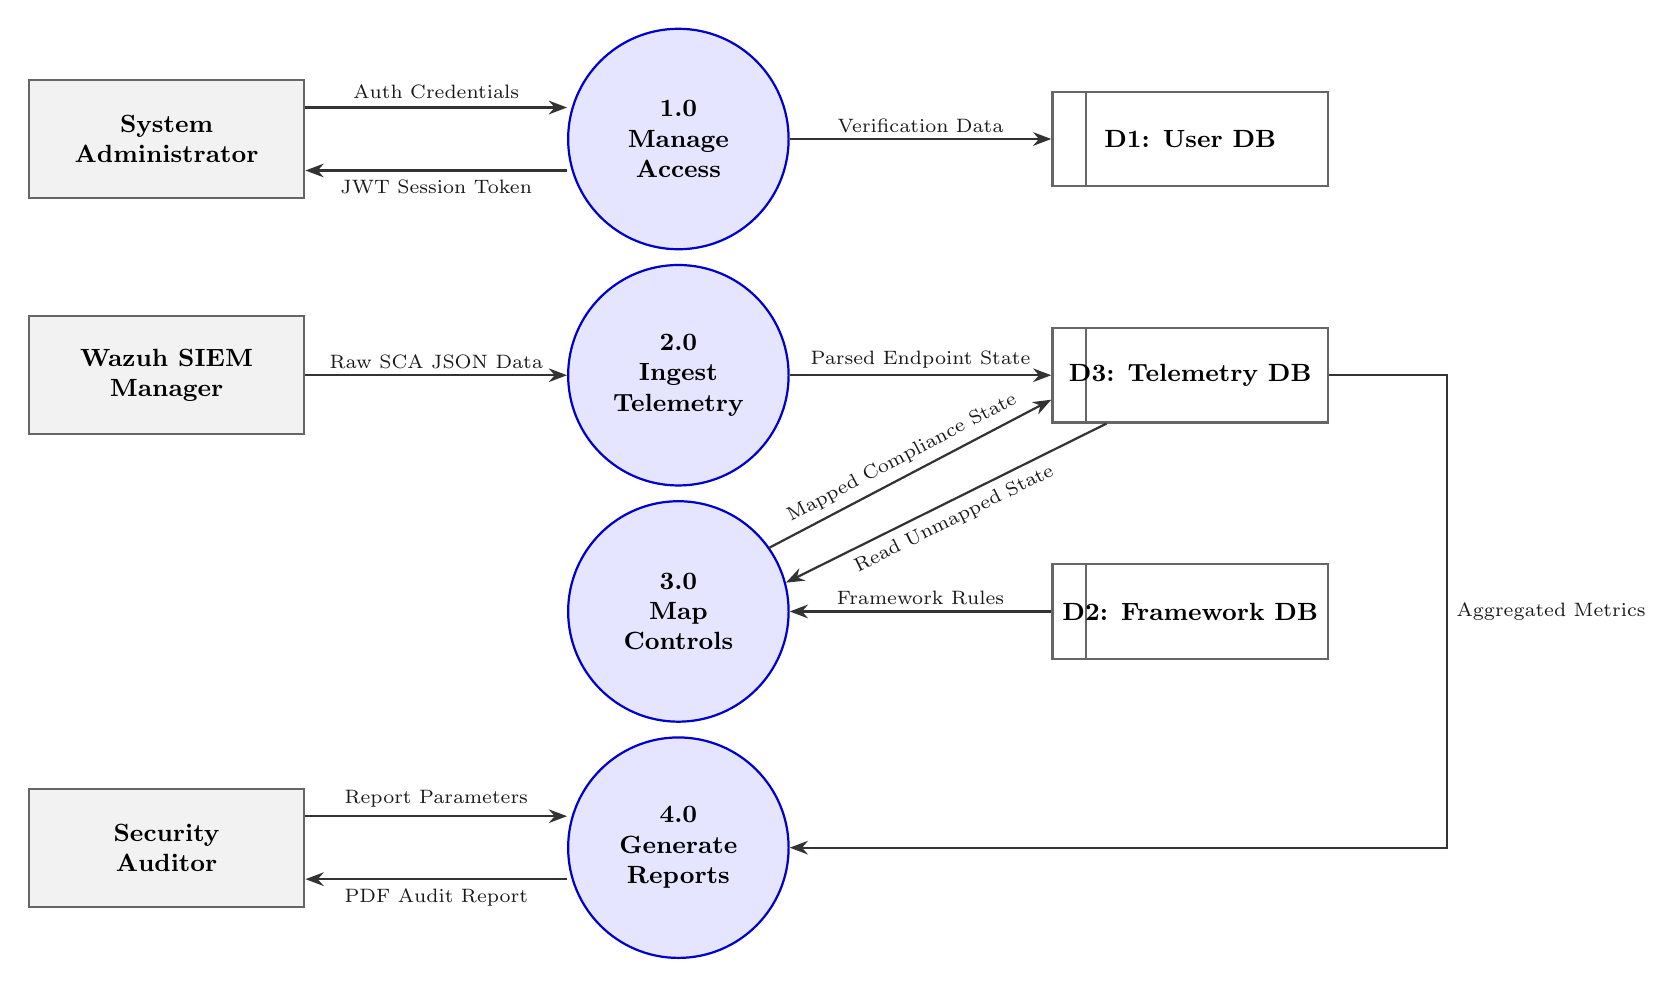
\begin{tikzpicture}[
        node distance=2.5cm,
        process/.style={circle, draw=blue!80!black, thick, fill=blue!10, minimum size=2.8cm, align=center, font=\bfseries\small},
        entity/.style={rectangle, draw=gray!80!black, thick, fill=gray!10, minimum width=3.5cm, minimum height=1.5cm, align=center, font=\bfseries\small},
        datastore/.style={rectangle, draw=gray!80!black, thick, fill=white, minimum width=3.5cm, minimum height=1.2cm, align=center, font=\bfseries\small, path picture={\draw[thick] ([xshift=12pt]path picture bounding box.north west) -- ([xshift=12pt]path picture bounding box.south west);}},
        flow/.style={-Stealth, thick, draw=black!80},
        flowlabel/.style={font=\scriptsize, align=center, text=black!90, inner sep=0pt}
    ]
        % External Entities (Left)
        \node[entity] (admin) at (-6.5, 4.5) {System\\Administrator};
        \node[entity] (wazuh) at (-6.5, 1.5) {Wazuh SIEM\\Manager};
        \node[entity] (auditor) at (-6.5, -4.5) {Security\\Auditor};

        % Processes (Center)
        \node[process] (p1) at (0, 4.5) {1.0\\Manage\\Access};
        \node[process] (p2) at (0, 1.5) {2.0\\Ingest\\Telemetry};
        \node[process] (p3) at (0, -1.5) {3.0\\Map\\Controls};
        \node[process] (p4) at (0, -4.5) {4.0\\Generate\\Reports};

        % Data Stores (Right)
        \node[datastore] (d1) at (6.5, 4.5) {D1: User DB};
        \node[datastore] (d3) at (6.5, 1.5) {D3: Telemetry DB};
        \node[datastore] (d2) at (6.5, -1.5) {D2: Framework DB};

        % Flows: Manage Access
        \draw[flow] ([yshift=4mm]admin.east) -- ([yshift=4mm]p1.west) node[midway, above=3pt, flowlabel] {Auth Credentials};
        \draw[flow] ([yshift=-4mm]p1.west) -- ([yshift=-4mm]admin.east) node[midway, below=3pt, flowlabel] {JWT Session Token};
        \draw[flow] (p1.east) -- (d1.west) node[midway, above=2pt, flowlabel] {Verification Data};

        % Flows: Ingest Telemetry
        \draw[flow] (wazuh.east) -- (p2.west) node[midway, above=2pt, flowlabel] {Raw SCA JSON Data};
        \draw[flow] (p2.east) -- (d3.west) node[midway, above=2pt, flowlabel] {Parsed Endpoint State};

        % Flows: Map Controls
        \draw[flow] (d2.west) -- (p3.east) node[midway, above=2pt, flowlabel] {Framework Rules};
        \draw[flow] (p3.35) -- (d3.190) node[midway, sloped, above=3pt, flowlabel] {Mapped Compliance State};
        \draw[flow] (d3.210) -- (p3.15) node[midway, sloped, below=3pt, flowlabel] {Read Unmapped State};

        % Flows: Generate Reports
        \draw[flow] ([yshift=4mm]auditor.east) -- ([yshift=4mm]p4.west) node[midway, above=3pt, flowlabel] {Report Parameters};
        \draw[flow] ([yshift=-4mm]p4.west) -- ([yshift=-4mm]auditor.east) node[midway, below=3pt, flowlabel] {PDF Audit Report};
        
        % Long-distance route from D3 to P4
        \draw[flow] (d3.east) -- ++(1.5,0) |- node[pos=0.25, right=3pt, flowlabel] {Aggregated Metrics} (p4.east);

    \end{tikzpicture}
    }
    \caption{Level-1 Data Flow Diagram detailing internal compliance processes.}
    \label{fig:dfd_level_1}
\end{figure}

\section{Use Cases}

The use cases define the interaction sequences available to authenticated actors, providing deterministic state definitions for platform operations.

\subsection{Use Case Diagram}

Figure \ref{fig:use_case_diagram} maps the operational workflows orchestrated by the System Administrator and the Security Auditor, establishing boundaries of execution based on the platform's internal RBAC implementation.

\begin{figure}[H]
    \centering
    \resizebox{\textwidth}{!}{
    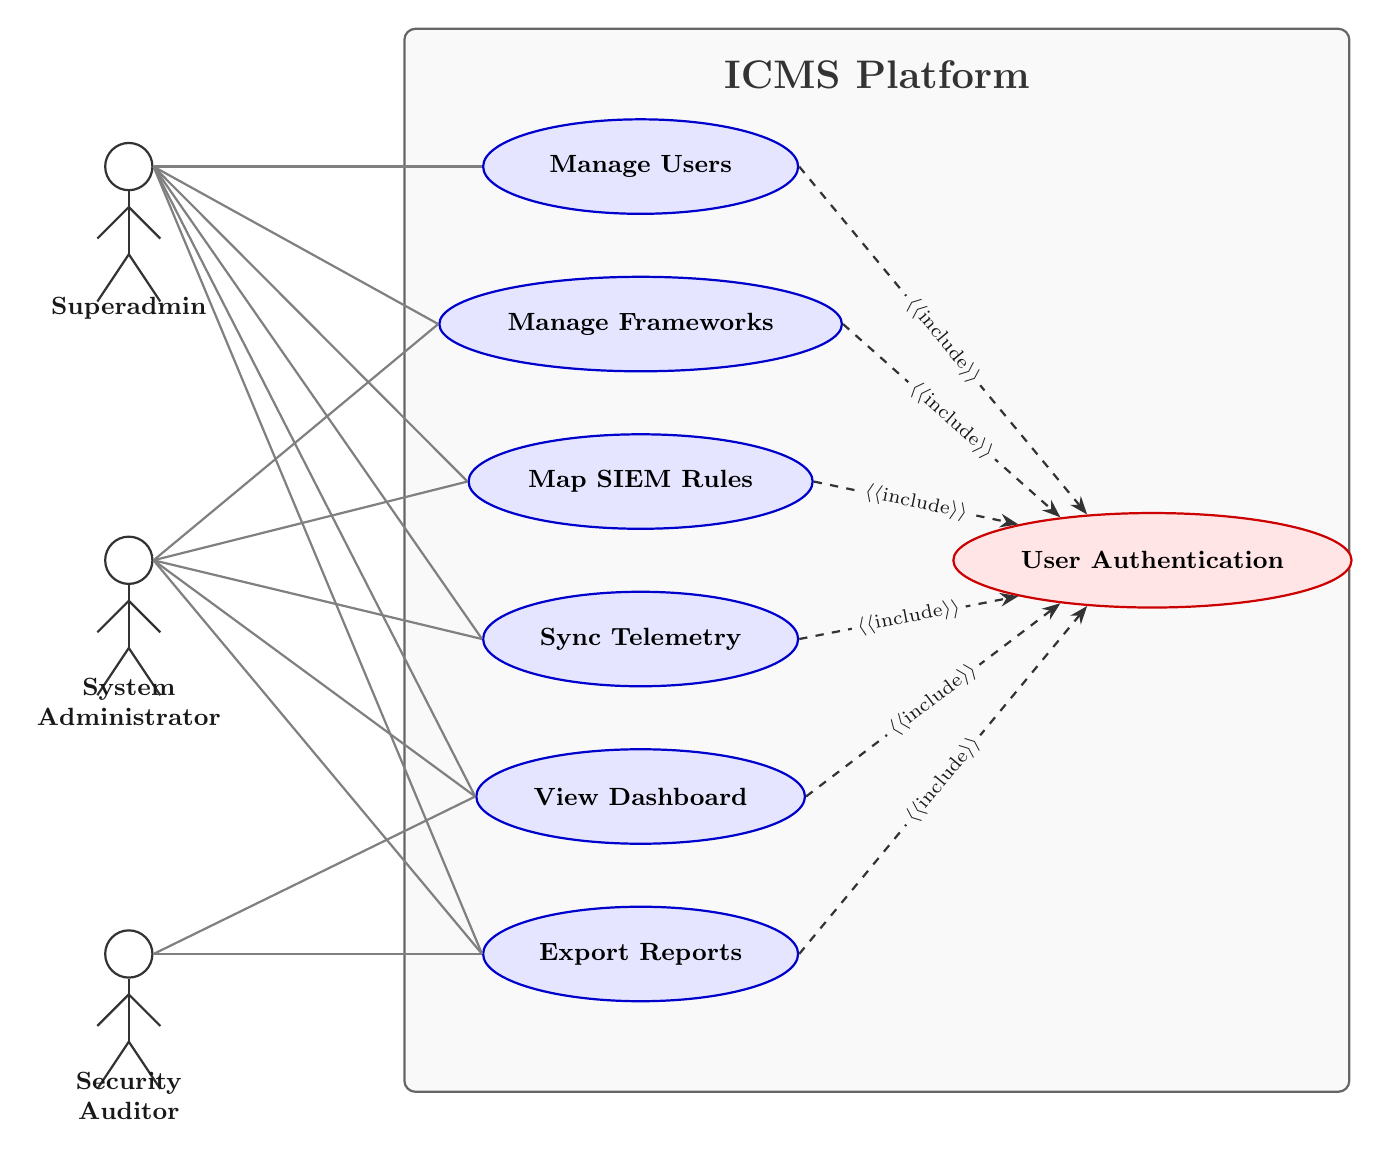
\begin{tikzpicture}[
        node distance=2cm,
        usecase/.style={ellipse, draw=blue!80!black, thick, fill=blue!10, minimum width=4cm, minimum height=1.2cm, align=center, font=\bfseries\small},
        authcase/.style={ellipse, draw=red!80!black, thick, fill=red!10, minimum width=4cm, minimum height=1.2cm, align=center, font=\bfseries\small},
        stickman/.style={circle, draw=black!80, thick, minimum size=6mm, fill=white,
            append after command={
                \pgfextra{
                    \draw[thick, draw=black!80] (\tikzlastnode.south) -- ++(0,-8mm) coordinate (body_bottom);
                    \draw[thick, draw=black!80] (\tikzlastnode.south) ++(0,-2mm) -- ++(-4mm,-4mm);
                    \draw[thick, draw=black!80] (\tikzlastnode.south) ++(0,-2mm) -- ++(4mm,-4mm);
                    \draw[thick, draw=black!80] (body_bottom) -- ++(-4mm,-6mm);
                    \draw[thick, draw=black!80] (body_bottom) -- ++(4mm,-6mm);
                }
            }
        },
        assoc/.style={thick, draw=black!50},
        include/.style={-Stealth, dashed, thick, draw=black!80},
        inclabel/.style={midway, fill=gray!5, font=\scriptsize, inner sep=2pt, text=black!90}
    ]
        % System Boundary
        \node[draw=gray!80!black, thick, minimum width=12cm, minimum height=13.5cm, fill=gray!5, rounded corners] (system) at (4.5, 0) {};
        \node[anchor=north, font=\bfseries\Large, yshift=-3mm, text=black!80] at (system.north) {ICMS Platform};

        % Actors (Left, well spaced to prevent line clipping)
        \node[stickman] (superadmin) at (-5, 5) {}; 
        \node[align=center, font=\bfseries\small, text=black!90] at (-5, 3.2) {Superadmin};

        \node[stickman] (admin) at (-5, 0) {}; 
        \node[align=center, font=\bfseries\small, text=black!90] at (-5, -1.8) {System\\Administrator};

        \node[stickman] (auditor) at (-5, -5) {}; 
        \node[align=center, font=\bfseries\small, text=black!90] at (-5, -6.8) {Security\\Auditor};

        % Primary Use Cases (Center)
        \node[usecase] (uc1) at (1.5, 5) {Manage Users};
        \node[usecase] (uc2) at (1.5, 3) {Manage Frameworks};
        \node[usecase] (uc3) at (1.5, 1) {Map SIEM Rules};
        \node[usecase] (uc4) at (1.5, -1) {Sync Telemetry};
        \node[usecase] (uc5) at (1.5, -3) {View Dashboard};
        \node[usecase] (uc6) at (1.5, -5) {Export Reports};

        % Included Auth Use Case (Right)
        \node[authcase] (ucauth) at (8, 0) {User Authentication};

        % Actor Associations
        % Superadmin
        \draw[assoc] (superadmin.east) -- (uc1.west);
        \draw[assoc] (superadmin.east) -- (uc2.west);
        \draw[assoc] (superadmin.east) -- (uc3.west);
        \draw[assoc] (superadmin.east) -- (uc4.west);
        \draw[assoc] (superadmin.east) -- (uc5.west);
        \draw[assoc] (superadmin.east) -- (uc6.west);

        % System Admin
        \draw[assoc] (admin.east) -- (uc2.west);
        \draw[assoc] (admin.east) -- (uc3.west);
        \draw[assoc] (admin.east) -- (uc4.west);
        \draw[assoc] (admin.east) -- (uc5.west);
        \draw[assoc] (admin.east) -- (uc6.west);

        % Auditor
        \draw[assoc] (auditor.east) -- (uc5.west);
        \draw[assoc] (auditor.east) -- (uc6.west);

        % Includes (using precise degree anchors to prevent overlap)
        \draw[include] (uc1.east) -- (ucauth.145) node[inclabel, sloped] {$\langle\langle$include$\rangle\rangle$};
        \draw[include] (uc2.east) -- (ucauth.155) node[inclabel, sloped] {$\langle\langle$include$\rangle\rangle$};
        \draw[include] (uc3.east) -- (ucauth.165) node[inclabel, sloped] {$\langle\langle$include$\rangle\rangle$};
        \draw[include] (uc4.east) -- (ucauth.195) node[inclabel, sloped] {$\langle\langle$include$\rangle\rangle$};
        \draw[include] (uc5.east) -- (ucauth.205) node[inclabel, sloped] {$\langle\langle$include$\rangle\rangle$};
        \draw[include] (uc6.east) -- (ucauth.215) node[inclabel, sloped] {$\langle\langle$include$\rangle\rangle$};
        
    \end{tikzpicture}
    }
    \caption{System Use Case Diagram}
    \label{fig:use_case_diagram}
\end{figure}

\subsection{Descriptive Use Cases}

The following tabular specifications define the algorithmic flows, authentication prerequisites, and resulting persistence states for each operation.

\renewcommand{\arraystretch}{1.5}
\begin{table}[H]
    \centering
    \caption{Use Case - Authentication}\label{tab:uc_01}
    \begin{tabular}{|>{\raggedright\arraybackslash}p{3cm}|p{11.5cm}|}
        \hline
        \textbf{Attribute} & \textbf{Description}\\
        \hline
        \textbf{Use Case ID} & UC-01 \\
        \hline
        \textbf{Use Case Name} & User Authentication \\
        \hline
        \textbf{Primary} \par \textbf{Actor} & System Administrator, Security Auditor \\
        \hline
        \textbf{Preconditions} & The user account is registered and active in the system. \\
        \hline
        \textbf{Main Flow} & 1. The user enters their credentials into the login interface.\newline 2. The system verifies the submitted credentials.\newline 3. The system grants access and displays the default dashboard view. \\
        \hline
        \textbf{Alternative Flows} & Invalid credentials \textrightarrow\ The system denies access and displays an authentication error message.\newline Session timeout \textrightarrow\ The system automatically refreshes the session without interrupting the user. \\
                \hline
        \textbf{Frequency of Use} & High (Initiated upon every new user session or token expiry). \\
        \hline
        \textbf{Priority} & Critical (Gatekeeper for all subsequent RBAC routing). \\
        \hline
        \textbf{Exception} & Account locked due to repeated invalid attempts \textrightarrow\ Deny access, log event to security audit trail, and prompt system administrator intervention. \\
\hline
        \textbf{Postconditions} & The user is successfully authenticated and an active session is established. \\
        \hline
    \end{tabular}
\end{table}

\begin{table}[H]
    \centering
    \caption{Use Case - Manage Frameworks}\label{tab:uc_02}
    \begin{tabular}{|>{\raggedright\arraybackslash}p{3cm}|p{11.5cm}|}
        \hline
        \textbf{Attribute} & \textbf{Description}\\
        \hline
        \textbf{Use Case ID} & UC-02 \\
        \hline
        \textbf{Use Case Name} & Manage Wazuh Telemetry Synchronization \\
        \hline
        \textbf{Primary} \par \textbf{Actor} & System Administrator \\
        \hline
        \textbf{Preconditions} & The Administrator is authenticated. $\langle\langle$include$\rangle\rangle$ User Authentication. The external SIEM system is reachable. \\
        \hline
        \textbf{Main Flow} & 1. The Administrator triggers a manual synchronization of security telemetry.\newline 2. The system requests audit data from the external SIEM.\newline 3. The system processes and maps the received data against the linked controls.\newline 4. The system updates the compliance status for each control.\newline 5. The system stores the audit results and notifies the Administrator. \\
        \hline
        \textbf{Alternative Flows} & SIEM system is unreachable \textrightarrow\ The system retries the connection and alerts the Administrator if it ultimately fails. \\
                \hline
        \textbf{Frequency of Use} & High (Continuous via Celery beat background tasks; occasional manual ad-hoc triggers by Superadmin). \\
        \hline
        \textbf{Priority} & Critical (Forms the core data ingestion pipeline for the compliance engine). \\
        \hline
        \textbf{Exception} & Wazuh REST API connection timeout or TLS handshake failure \textrightarrow\ Abort sync, log connection error, and queue retry via Celery exponential backoff. \\
\hline
        \textbf{Postconditions} & The system reflects the latest compliance state based on the synchronized SIEM data. \\
        \hline
    \end{tabular}
\end{table}

\begin{table}[H]
    \centering
    \caption{Use Case - Map Controls}\label{tab:uc_03}
    \begin{tabular}{|>{\raggedright\arraybackslash}p{3cm}|p{11.5cm}|}
        \hline
        \textbf{Attribute} & \textbf{Description}\\
        \hline
        \textbf{Use Case ID} & UC-03 \\
        \hline
        \textbf{Use Case Name} & Map Framework Controls to Wazuh Rules \\
        \hline
        \textbf{Primary} \par \textbf{Actor} & System Administrator \\
        \hline
        \textbf{Preconditions} & The Administrator is authenticated. $\langle\langle$include$\rangle\rangle$ User Authentication. Frameworks and controls exist in the system. \\
        \hline
        \textbf{Main Flow} & 1. The Administrator selects a SIEM rule and links it to a specific compliance control.\newline 2. The system validates the relationship between the rule and the control.\newline 3. The system saves the mapping configuration.\newline 4. The system confirms the successful linkage to the Administrator. \\
        \hline
        \textbf{Alternative Flows} & Invalid control selected \textrightarrow\ The system rejects the mapping and prompts the Administrator to select a valid control. \\
                \hline
        \textbf{Frequency of Use} & Low/Medium (Executed during initial platform setup or when regulatory frameworks release new versions). \\
        \hline
        \textbf{Priority} & High (Defines the relational logic for the entire compliance evaluation). \\
        \hline
        \textbf{Exception} & Mapping collision or invalid/deprecated Wazuh Rule ID \textrightarrow\ Prevent database commit, display strict validation error to the Superadmin. \\
\hline
        \textbf{Postconditions} & A linkage is established between the SIEM rule and the compliance control for future audits. \\
        \hline
    \end{tabular}
\end{table}

\begin{table}[H]
    \centering
    \caption{Use Case - Sync Telemetry}\label{tab:uc_04}
    \begin{tabular}{|>{\raggedright\arraybackslash}p{3cm}|p{11.5cm}|}
        \hline
        \textbf{Attribute} & \textbf{Description}\\
        \hline
        \textbf{Use Case ID} & UC-04 \\
        \hline
        \textbf{Use Case Name} & Monitor Endpoint Compliance Status \\
        \hline
        \textbf{Primary} \par \textbf{Actor} & System Administrator (Trigger) / Celery (System Actor) \\
        \hline
        \textbf{Preconditions} & The user is authenticated. $\langle\langle$include$\rangle\rangle$ User Authentication. \\
        \hline
        \textbf{Main Flow} & 1. The user navigates to the dashboard view.\newline 2. The system aggregates the latest compliance data.\newline 3. The system visualizes the compliance score and detailed control statuses. \\
        \hline
        \textbf{Alternative Flows} & No data available \textrightarrow\ The system displays an empty state with a prompt to synchronize telemetry. \\
                \hline
        \textbf{Frequency of Use} & High (Serves as the primary operational dashboard for continuous monitoring). \\
        \hline
        \textbf{Priority} & High (Core visibility and monitoring function). \\
        \hline
        \textbf{Exception} & Endpoint agent disconnected or offline \textrightarrow\ Mark endpoint status as 'Stale/Offline', visually highlight the disconnection in the UI, and suspend compliance calculations for that node. \\
\hline
        \textbf{Postconditions} & The user is presented with an up-to-date visual compliance posture. \\
        \hline
    \end{tabular}
\end{table}

\begin{table}[H]
    \centering
    \caption{Use Case - View Dashboard}\label{tab:uc_05}
    \begin{tabular}{|>{\raggedright\arraybackslash}p{3cm}|p{11.5cm}|}
        \hline
        \textbf{Attribute} & \textbf{Description}\\
        \hline
        \textbf{Use Case ID} & UC-05 \\
        \hline
        \textbf{Use Case Name} & Resolve Compliance Anomalies \\
        \hline
        \textbf{Primary} \par \textbf{Actor} & Security Auditor, System Administrator \\
        \hline
        \textbf{Preconditions} & The Auditor or Admin is authenticated. Compliance failures have been detected in the system. \\
        \hline
        \textbf{Main Flow} & 1. The user identifies a non-compliant control on the dashboard.\newline 2. The user initiates a resolution workflow and applies corrective actions to the endpoint.\newline 3. The system verifies the change and logs the remediation status. \\
        \hline
        \textbf{Alternative Flows} & Resolution fails \textrightarrow\ The system maintains the 'Failed' state and prompts for manual investigation. \\
                \hline
        \textbf{Frequency of Use} & Medium (Event-driven, based on incoming alerts and failed states). \\
        \hline
        \textbf{Priority} & Medium/High (Critical for operational remediation, but dependent on external IT actions). \\
        \hline
        \textbf{Exception} & Insufficient RBAC permissions to apply resolution (e.g., Auditor attempting Admin action) \textrightarrow\ Deny action, return HTTP 403 Forbidden, and log unauthorized attempt. \\
\hline
        \textbf{Postconditions} & The compliance anomaly is resolved and recorded in the historical audit ledger. \\
        \hline
    \end{tabular}
\end{table}

\begin{table}[H]
    \centering
    \caption{Use Case - Export Audit Reports}\label{tab:uc_06}
    \begin{tabular}{|>{\raggedright\arraybackslash}p{3cm}|p{11.5cm}|}
        \hline
        \textbf{Attribute} & \textbf{Description}\\
        \hline
        \textbf{Use Case ID} & UC-06 \\
        \hline
        \textbf{Use Case Name} & Export Audit Reports \\
        \hline
        \textbf{Primary} \par \textbf{Actor} & Security Auditor \\
        \hline
        \textbf{Preconditions} & The Auditor is authenticated. $\langle\langle$include$\rangle\rangle$ User Authentication. Compliance data exists. \\
        \hline
        \textbf{Main Flow} & 1. The Auditor requests a formal compliance report for a specific framework.\newline 2. The system compiles the historical audit data.\newline 3. The system generates a formatted PDF document.\newline 4. The system prompts the Auditor to download the document. \\
        \hline
        \textbf{Alternative Flows} & Generation failure \textrightarrow\ The system displays a generation error message and logs the failure. \\
                \hline
        \textbf{Frequency of Use} & Low (Triggered periodically based on audit cycles, e.g., monthly or quarterly). \\
        \hline
        \textbf{Priority} & High (Primary executive deliverable for external governance bodies). \\
        \hline
        \textbf{Exception} & PostgreSQL data retrieval timeout or PDF template rendering failure \textrightarrow\ Abort generation, display generic error modal, and log backend stack trace. \\
\hline
        \textbf{Postconditions} & A timestamped audit report is delivered to the Auditor. \\
        \hline

    \end{tabular}
\end{table}

% \chapter{Design}

\section{System Architecture}
The Intelligent Security Compliance Management System (ISCMS) uses an N-tier architecture. Separating the frontend, API, background workers, and database allows for scaling and debugging of individual components without affecting the entire system. Figure \ref{fig:tier_architecture} shows the four main layers.

\subsection{Client and Presentation Tier}
The frontend is a React 18 Single Page Application (SPA). Moving the rendering logic to the browser reduces server load and lets analysts review compliance alerts without full page reloads.

\subsection{Application and Middleware Tier}
The backend uses the Django REST Framework. It is the primary gateway, verifying JWTs and enforcing role-based access before processing queries. Database traffic is routed through Django to maintain a consistent security boundary.

\subsection{Asynchronous Processing Tier}
Retrieving telemetry from the Wazuh SIEM is an I/O-intensive process. Executing these tasks on the main Django thread would cause API latency and timeouts. To prevent this, the system offloads I/O tasks to background Celery workers using Redis as the message broker.

\subsection{Data Persistence Tier}
PostgreSQL 18 is the primary database for its ACID guarantees. The schema uses relational tables for mapping frameworks to controls, while the JSONField type stores unstructured SIEM logs.

\begin{figure}[H]
    \centering
    \resizebox{0.85\textwidth}{!}{
    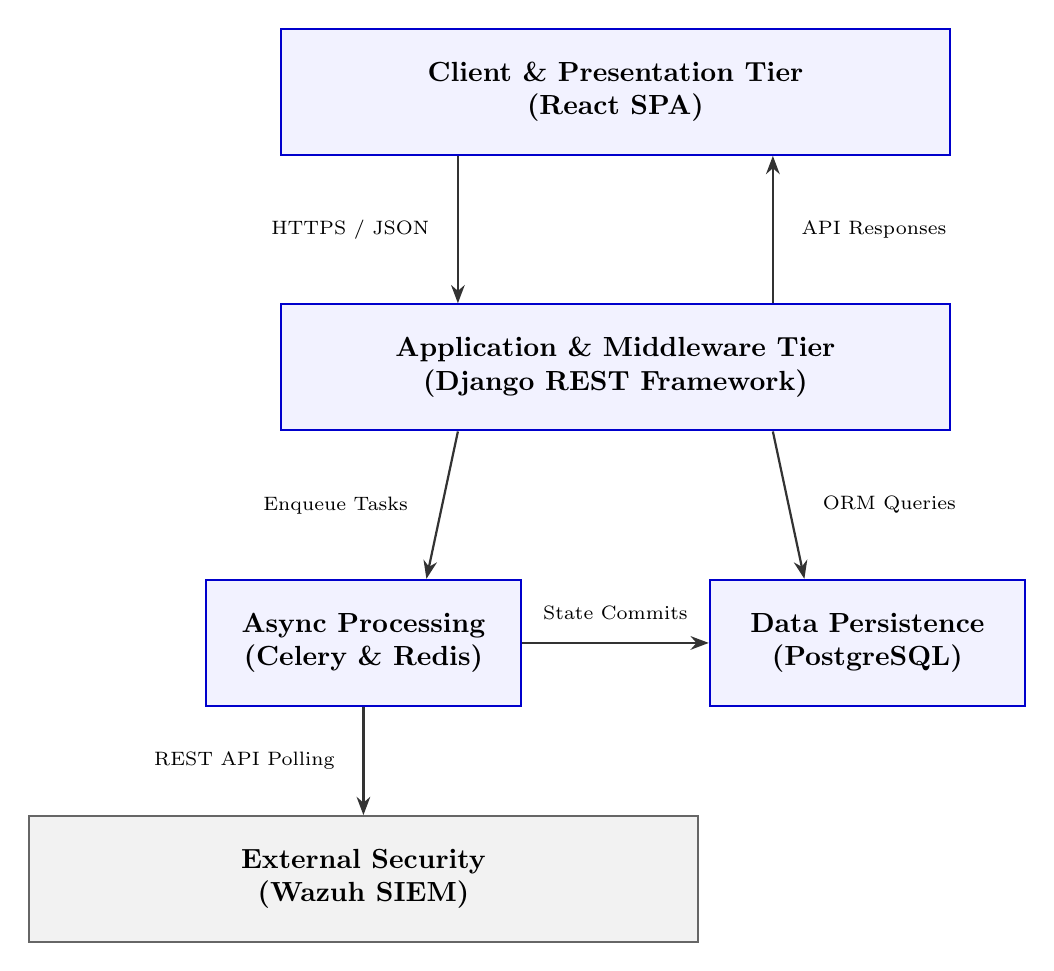
\begin{tikzpicture}[
        tier/.style={rectangle, draw=blue!80!black, thick, fill=blue!5, minimum width=8.5cm, minimum height=1.6cm, align=center, font=\bfseries},
        arrow/.style={-Stealth, thick, draw=black!80},
        label/.style={font=\scriptsize, inner sep=2pt}
    ]
        % Tiers with increased separation to resolve congestion
        \node[tier] (client) at (0, 8.5) {Client \& Presentation Tier\\(React SPA)};
        \node[tier] (app) at (0, 5.0) {Application \& Middleware Tier\\(Django REST Framework)};
        
        \node[tier, minimum width=4cm] (async) at (-3.2, 1.5) {Async Processing\\(Celery \& Redis)};
        \node[tier, minimum width=4cm] (data) at (3.2, 1.5) {Data Persistence\\(PostgreSQL)};
        
        \node[tier, fill=gray!10, draw=gray!80!black] (wazuh) at (-3.2, -1.5) {External Security\\(Wazuh SIEM)};

        % Client <-> App Connections
        \draw[arrow] ([xshift=-2cm]client.south) -- ([xshift=-2cm]app.north) 
            node[midway, left=8pt, label] {HTTPS / JSON};
        \draw[arrow] ([xshift=2cm]app.north) -- ([xshift=2cm]client.south) 
            node[midway, right=8pt, label] {API Responses};

        % App -> Async / Data Connections (Widened entry points)
        \draw[arrow] ([xshift=-2cm]app.south) -- ([xshift=0.8cm]async.north) 
            node[midway, left=10pt, label] {Enqueue Tasks};
        \draw[arrow] ([xshift=2cm]app.south) -- ([xshift=-0.8cm]data.north) 
            node[midway, right=10pt, label] {ORM Queries};

        % Async -> Wazuh (Increased vertical gap)
        \draw[arrow] (async.south) -- (wazuh.north) 
            node[midway, left=8pt, label] {REST API Polling};
        
        % Async -> Data (Increased horizontal gap)
        \draw[arrow] (async.east) -- (data.west) 
            node[midway, above=6pt, label] {State Commits};
    \end{tikzpicture}
    }
    \caption{Tier-wise System Architecture of the ISCMS Platform}
    \label{fig:tier_architecture}
\end{figure}

\section{Design Constraints}
The design of the ISCMS involved addressing several technical and environmental constraints.

\subsection{Technical Constraints}
For security, the database and Redis broker operate inside a private Docker bridge network. Their ports are not exposed to the host machine. Access to data requires requests through the Django API container.

The integration with the Wazuh API introduced rate limits and network latency. Celery workers are configured to batch and throttle polling requests. Consequently, the dashboard displays the compliance state from the last successful synchronization rather than a real-time feed.

On the frontend, rendering large compliance grids can impact browser performance. Loading thousands of DOM nodes simultaneously can block the main thread. React virtualization addresses this by rendering only the visible elements.

\subsection{Infrastructure and Operational Constraints}
External factors, such as restricted access to university facilities, required the transition to developing and testing the architecture in a home-lab environment.

Running a full Wazuh SIEM manager locally is resource-intensive and can impact system stability. To manage this, a distributed configuration was used. One system was dedicated to running Wazuh, while another was used for development and as a monitored endpoint. Git was used to maintain consistency across different development environments while the primary infrastructure remained on a dedicated server.

\section{Design Methodology}
The platform was built using an iterative prototyping approach. The system was divided into distinct modules to allow for independent testing before integration.

The project was divided into four main phases:

\begin{itemize}
    \item \textbf{Phase 1 (Prototyping):} The initial phase focused on verifying the core concept. This included setting up a basic Django backend and testing the Wazuh API to confirm successful retrieval of Security Configuration Assessment (SCA) telemetry.
    
    \item \textbf{Phase 2 (Core Architecture):} The second phase involved designing the PostgreSQL database schema to link frameworks to rules. JWT authentication and role-based routing were also implemented to secure the API.
    
    \item \textbf{Phase 3 (Asynchronous Telemetry):} Celery and Redis were added to handle heavy SIEM data ingestion. This established a background worker fleet for data processing and deduplication.
    
    \item \textbf{Phase 4 (Frontend \& Visualization):} The final phase involved building the React frontend. This included rendering data grids, implementing state management, and configuring the server-side PDF generator for audit reports.
\end{itemize}

\section{High Level Design}
The system architecture is represented through several views that cover software components, physical deployment, and operational sequences.

\subsection{Component Diagram}
Figure \ref{fig:component_diagram} shows the interactions between system modules. The React frontend sends HTTPS requests to the Django API Gateway. The IAM module verifies the JWT, and the Compliance Engine then translates the request into a database query. A separate Wazuh Polling Service retrieves alerts and stores them in PostgreSQL.

\begin{figure}[H]
    \centering
    \resizebox{0.9\textwidth}{!}{
    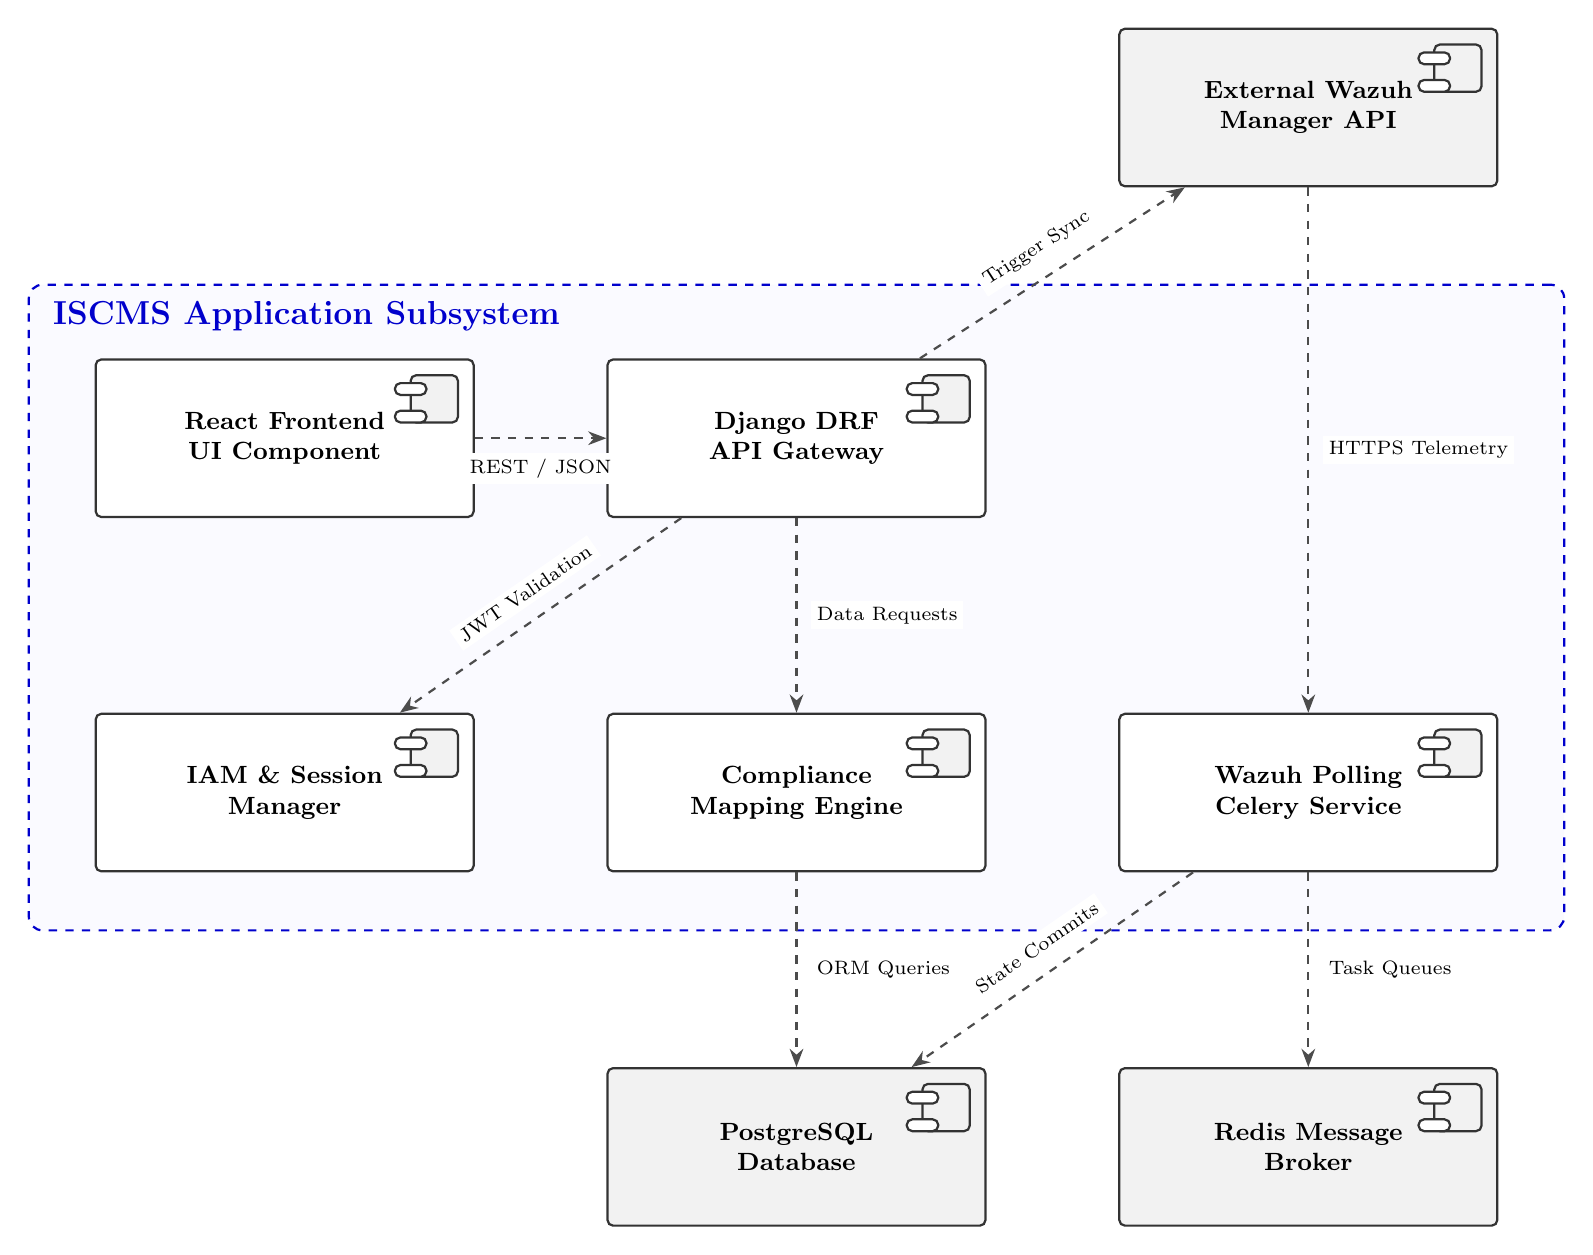
\begin{tikzpicture}[
        comp/.style={rectangle, draw=black!80, thick, fill=white, minimum width=4.8cm, minimum height=2cm, text width=3.8cm, align=center, font=\small\bfseries, rounded corners=2pt,
            path picture={
                \draw[black!80, thick, fill=gray!10] ([xshift=-8mm,yshift=-2mm]path picture bounding box.north east) rectangle ++(6mm,-6mm);
                \draw[black!80, thick, fill=white] ([xshift=-10mm,yshift=-3mm]path picture bounding box.north east) rectangle ++(4mm,-1.5mm);
                \draw[black!80, thick, fill=white] ([xshift=-10mm,yshift=-6.5mm]path picture bounding box.north east) rectangle ++(4mm,-1.5mm);
            }
        },
        extcomp/.style={comp, fill=gray!10},
        arrow/.style={-Stealth, thick, dashed, draw=black!70},
        label/.style={font=\scriptsize, fill=white, inner sep=2pt}
    ]
        % System Boundary (Shifted up slightly for title clearance)
        \node[draw=blue!80!black, thick, minimum width=19.5cm, minimum height=8.2cm, fill=blue!2, rounded corners=5pt, dashed] (system) at (3, 0.85) {};
        \node[anchor=north west, xshift=2mm, yshift=-1mm, font=\bfseries\large, text=blue!80!black] at (system.north west) {ISCMS Application Subsystem};

        % ROW 0: External Top
        \node[extcomp] (wazuh) at (9.5, 7.2) {External Wazuh\\Manager API};

        % ROW 1: Internal Top
        \node[comp] (ui) at (-3.5, 3) {React Frontend\\UI Component};
        \node[comp] (gateway) at (3, 3) {Django DRF\\API Gateway};
        
        % ROW 2: Internal Bottom
        \node[comp] (auth) at (-3.5, -1.5) {IAM \& Session\\Manager};
        \node[comp] (engine) at (3, -1.5) {Compliance\\Mapping Engine};
        \node[comp] (poll) at (9.5, -1.5) {Wazuh Polling\\Celery Service};

        % ROW 3: External Bottom
        \node[extcomp] (db) at (3, -6) {PostgreSQL\\Database};
        \node[extcomp] (redis) at (9.5, -6) {Redis Message\\Broker};

        % Dependencies
        \draw[arrow] (ui) -- (gateway) node[midway, below=5pt, label] {REST / JSON};
        \draw[arrow] (gateway) -- (auth) node[midway, above=5pt, label, sloped] {JWT Validation};
        \draw[arrow] (gateway) -- (engine) node[midway, right=5pt, label] {Data Requests};
        \draw[arrow] (gateway) -- (wazuh) node[midway, above=5pt, label, sloped] {Trigger Sync};
        \draw[arrow] (wazuh) -- (poll) node[midway, right=5pt, label] {HTTPS Telemetry};
        
        \draw[arrow] (engine) -- (db) node[midway, right=5pt, label] {ORM Queries};
        \draw[arrow] (poll) -- (db) node[midway, above=5pt, label, sloped] {State Commits};
        \draw[arrow] (poll) -- (redis) node[midway, right=5pt, label] {Task Queues};
    \end{tikzpicture}
    }
    \caption{Conceptual View: UML Component Diagram}
    \label{fig:component_diagram}
\end{figure}

\subsection{Deployment Diagram}
Figure \ref{fig:deployment_diagram} outlines the Docker container environment. The Django backend, Celery workers, Redis, and PostgreSQL are deployed on the same host but isolated within a private bridge network. This keeps the database inaccessible from external networks.

\begin{figure}[H]
    \centering
    \resizebox{0.95\textwidth}{!}{
    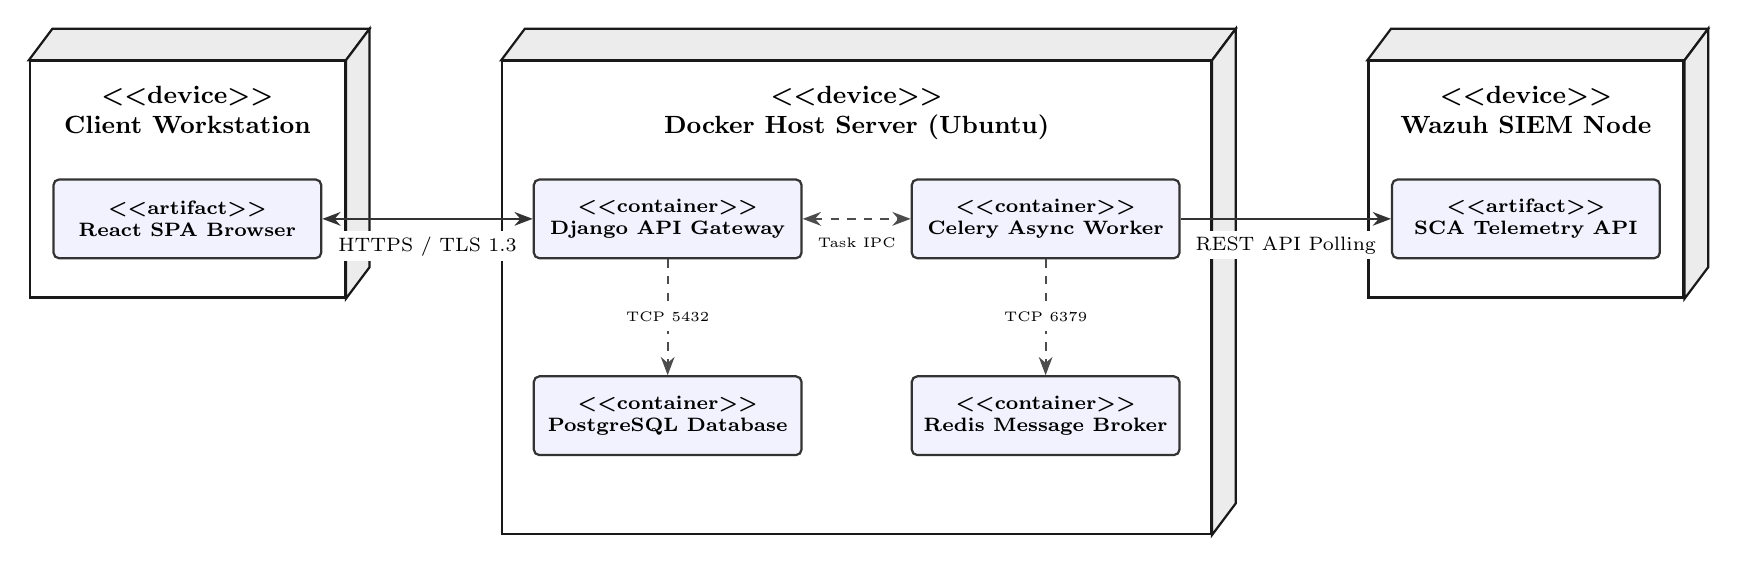
\begin{tikzpicture}[
        device/.style={
            rectangle, draw=black!90, thick, fill=white,
            minimum width=4cm, minimum height=2.5cm,
            append after command={
                \pgfextra{
                    \filldraw[black!90, thick, fill=gray!15] (\tikzlastnode.north west) -- ++(0.3, 0.4) -- ($(\tikzlastnode.north east)+(0.3,0.4)$) -- (\tikzlastnode.north east) -- cycle;
                    \filldraw[black!90, thick, fill=gray!15] (\tikzlastnode.north east) -- ($(\tikzlastnode.north east)+(0.3,0.4)$) -- ($(\tikzlastnode.south east)+(0.3,0.4)$) -- (\tikzlastnode.south east) -- cycle;
                }
            }
        },
        artifact/.style={
            rectangle, draw=black!80, thick, fill=blue!5,
            minimum width=3.4cm, minimum height=1cm,
            align=center, font=\scriptsize\bfseries, rounded corners=2pt
        },
        conn/.style={
            thick, draw=black!80, Stealth-Stealth
        },
        label/.style={
            font=\scriptsize, fill=white, inner sep=2pt
        }
    ]
        % ----------------------------------------------------
        % CENTER: Docker Host Server
        % ----------------------------------------------------
        \node[device, minimum width=9cm, minimum height=6cm] (server) at (0, 0) {};
        \node[anchor=north, font=\small\bfseries, yshift=-2mm, align=center] at (server.north) {\textless\textless device\textgreater\textgreater\\Docker Host Server (Ubuntu)};
        
        \node[artifact] (django) at (-2.4, 1) {\textless\textless container\textgreater\textgreater\\Django API Gateway};
        \node[artifact] (celery) at (2.4, 1) {\textless\textless container\textgreater\textgreater\\Celery Async Worker};
        \node[artifact] (postgres) at (-2.4, -1.5) {\textless\textless container\textgreater\textgreater\\PostgreSQL Database};
        \node[artifact] (redis) at (2.4, -1.5) {\textless\textless container\textgreater\textgreater\\Redis Message Broker};

        % Internal Bridge Network Connections
        \draw[dashed, -Stealth, thick, draw=black!70] (django.south) -- (postgres.north) node[midway, fill=white, font=\tiny] {TCP 5432};
        \draw[dashed, -Stealth, thick, draw=black!70] (celery.south) -- (redis.north) node[midway, fill=white, font=\tiny] {TCP 6379};
        \draw[dashed, Stealth-Stealth, thick, draw=black!70] (django.east) -- (celery.west) node[midway, below=3pt, fill=white, font=\tiny] {Task IPC};

        % ----------------------------------------------------
        % LEFT: Client Workstation
        % ----------------------------------------------------
        \node[device, minimum width=4cm, minimum height=3cm] (client) at (-8.5, 1.5) {};
        \node[anchor=north, font=\small\bfseries, yshift=-2mm, align=center] at (client.north) {\textless\textless device\textgreater\textgreater\\Client Workstation};
        \node[artifact] (react) at (-8.5, 1) {\textless\textless artifact\textgreater\textgreater\\React SPA Browser};

        % ----------------------------------------------------
        % RIGHT: Wazuh SIEM Node
        % ----------------------------------------------------
        \node[device, minimum width=4cm, minimum height=3cm] (wazuh) at (8.5, 1.5) {};
        \node[anchor=north, font=\small\bfseries, yshift=-2mm, align=center] at (wazuh.north) {\textless\textless device\textgreater\textgreater\\Wazuh SIEM Node};
        \node[artifact] (sca) at (8.5, 1) {\textless\textless artifact\textgreater\textgreater\\SCA Telemetry API};

        % ----------------------------------------------------
        % EXTERNAL NETWORK CONNECTIONS (Perfectly Horizontal at Y=1)
        % ----------------------------------------------------
        \draw[conn] (react.east) -- (django.west) node[midway, below=4pt, label] {HTTPS / TLS 1.3};
        \draw[conn, -Stealth] (celery.east) -- (sca.west) node[midway, below=4pt, label] {REST API Polling};

    \end{tikzpicture}
    }
    \caption{Physical View: UML Deployment Diagram}
    \label{fig:deployment_diagram}
\end{figure}

\subsection{System Activity Diagrams}
The activity diagrams below show the control flow for core platform features. Standard UML semantics, such as decision nodes and synchronization forks, are used to represent the system logic.

\subsubsection{Authentication and IAM Routing}
Figure \ref{fig:activity_auth} shows the login process. Django verifies credentials against PostgreSQL. If the verification fails, the system logs the event and denies the request. Upon successful authentication, the system issues a JWT and evaluates the user's role. Administrators are directed to configuration settings, while Auditors are restricted to read-only dashboards.

\begin{figure}[H]
    \centering
    \resizebox{0.75\textwidth}{!}{
    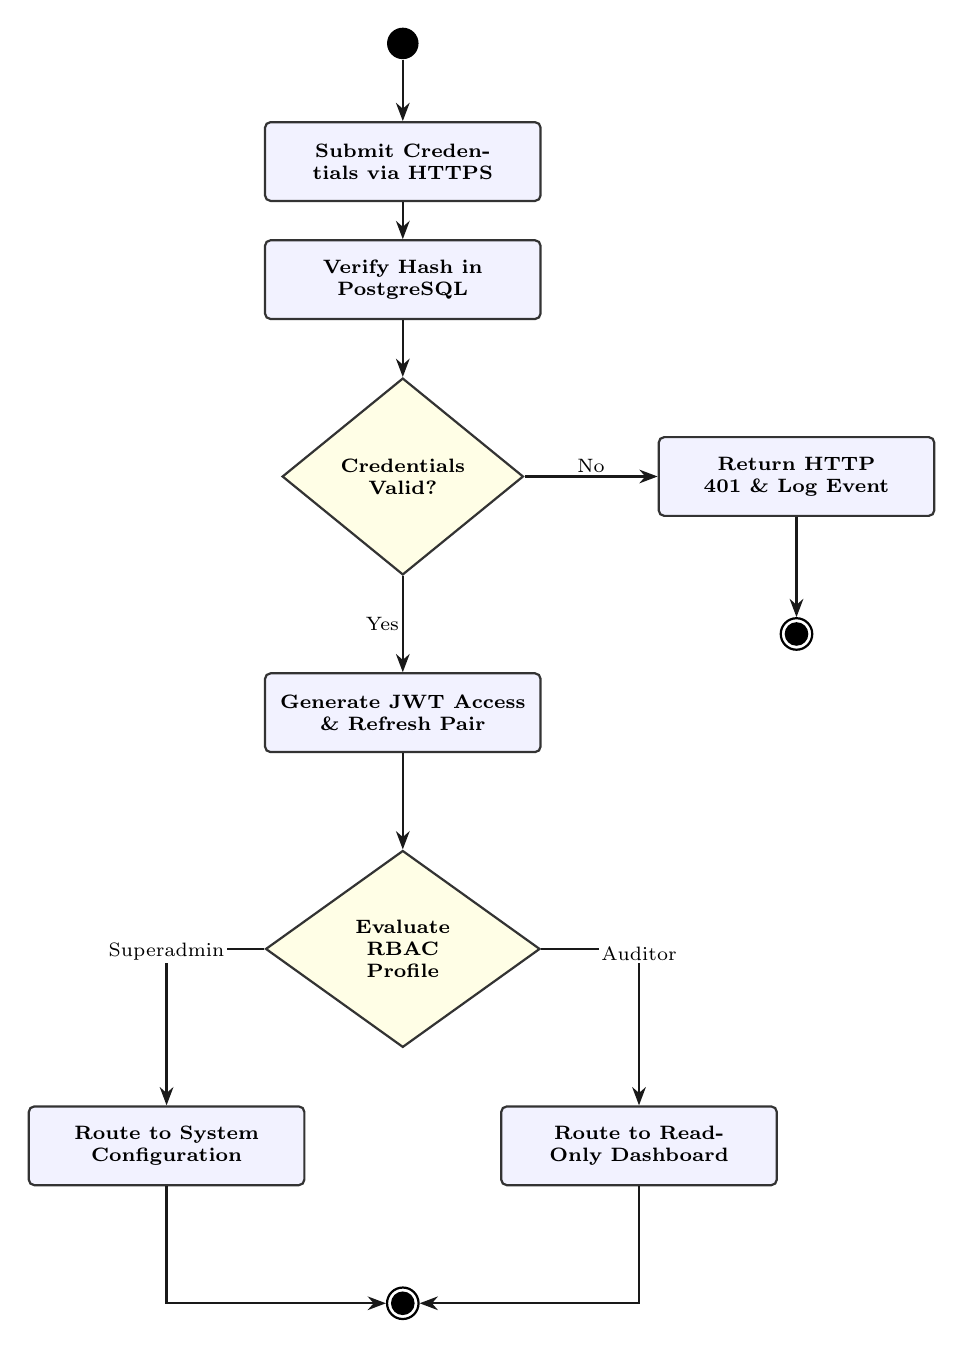
\begin{tikzpicture}[
        node distance=1.5cm,
        startstop/.style={circle, fill=black, minimum size=0.4cm},
        end/.style={circle, draw=black, thick, minimum size=0.4cm, path picture={\fill[black] (path picture bounding box.center) circle (0.15cm);}},
        activity/.style={rectangle, draw=black!80, thick, fill=blue!5, minimum width=3.5cm, minimum height=1cm, align=center, font=\scriptsize\bfseries, rounded corners=2pt, text width=3.2cm},
        decision/.style={diamond, draw=black!80, thick, fill=yellow!10, minimum width=2.5cm, minimum height=2.5cm, align=center, font=\scriptsize\bfseries, aspect=1.5, text width=1.8cm},
        arrow/.style={-Stealth, thick, draw=black!90},
        label/.style={font=\scriptsize, fill=white, inner sep=1pt}
    ]
        \node[startstop] (start) at (0,0) {};
        \node[activity] (submit) at (0,-1.5) {Submit Credentials via HTTPS};
        \node[activity] (verify) at (0,-3) {Verify Hash in PostgreSQL};
        \node[decision] (isvalid) at (0,-5.5) {Credentials Valid?};
        \node[activity] (reject) at (5,-5.5) {Return HTTP 401 \& Log Event};
        \node[activity] (jwt) at (0,-8.5) {Generate JWT Access \& Refresh Pair};
        \node[decision] (role) at (0,-11.5) {Evaluate RBAC Profile};
        \node[activity] (admin) at (-3,-14) {Route to System Configuration};
        \node[activity] (auditor) at (3,-14) {Route to Read-Only Dashboard};
        \node[end] (end1) at (5,-7.5) {};
        \node[end] (end2) at (0,-16) {};

        \draw[arrow] (start) -- (submit);
        \draw[arrow] (submit) -- (verify);
        \draw[arrow] (verify) -- (isvalid);
        \draw[arrow] (isvalid) -- (reject) node[midway, above, label] {No};
        \draw[arrow] (reject) -- (end1);
        \draw[arrow] (isvalid) -- (jwt) node[midway, left, label] {Yes};
        \draw[arrow] (jwt) -- (role);
        \draw[arrow] (role) -| (admin) node[pos=0.55, above, label] {Superadmin};
        \draw[arrow] (role) -| (auditor) node[pos=0.55, above, label] {Auditor};
        \draw[arrow] (admin) |- (end2);
        \draw[arrow] (auditor) |- (end2);
    \end{tikzpicture}
    }
    \caption{Activity Diagram: Authentication and IAM Routing}
    \label{fig:activity_auth}
\end{figure}

\subsubsection{Asynchronous Telemetry Ingestion}
Figure \ref{fig:activity_sync} shows the asynchronous ingestion process. When a synchronization task is triggered, the main thread returns an HTTP 202 status to the client. Simultaneously, the Celery worker polls the Wazuh API. If the SIEM is unreachable, the system uses exponential backoff. Once telemetry is retrieved, the system parses the JSON data and updates the database.

\begin{figure}[H]
    \centering
    \resizebox{0.8\textwidth}{!}{
    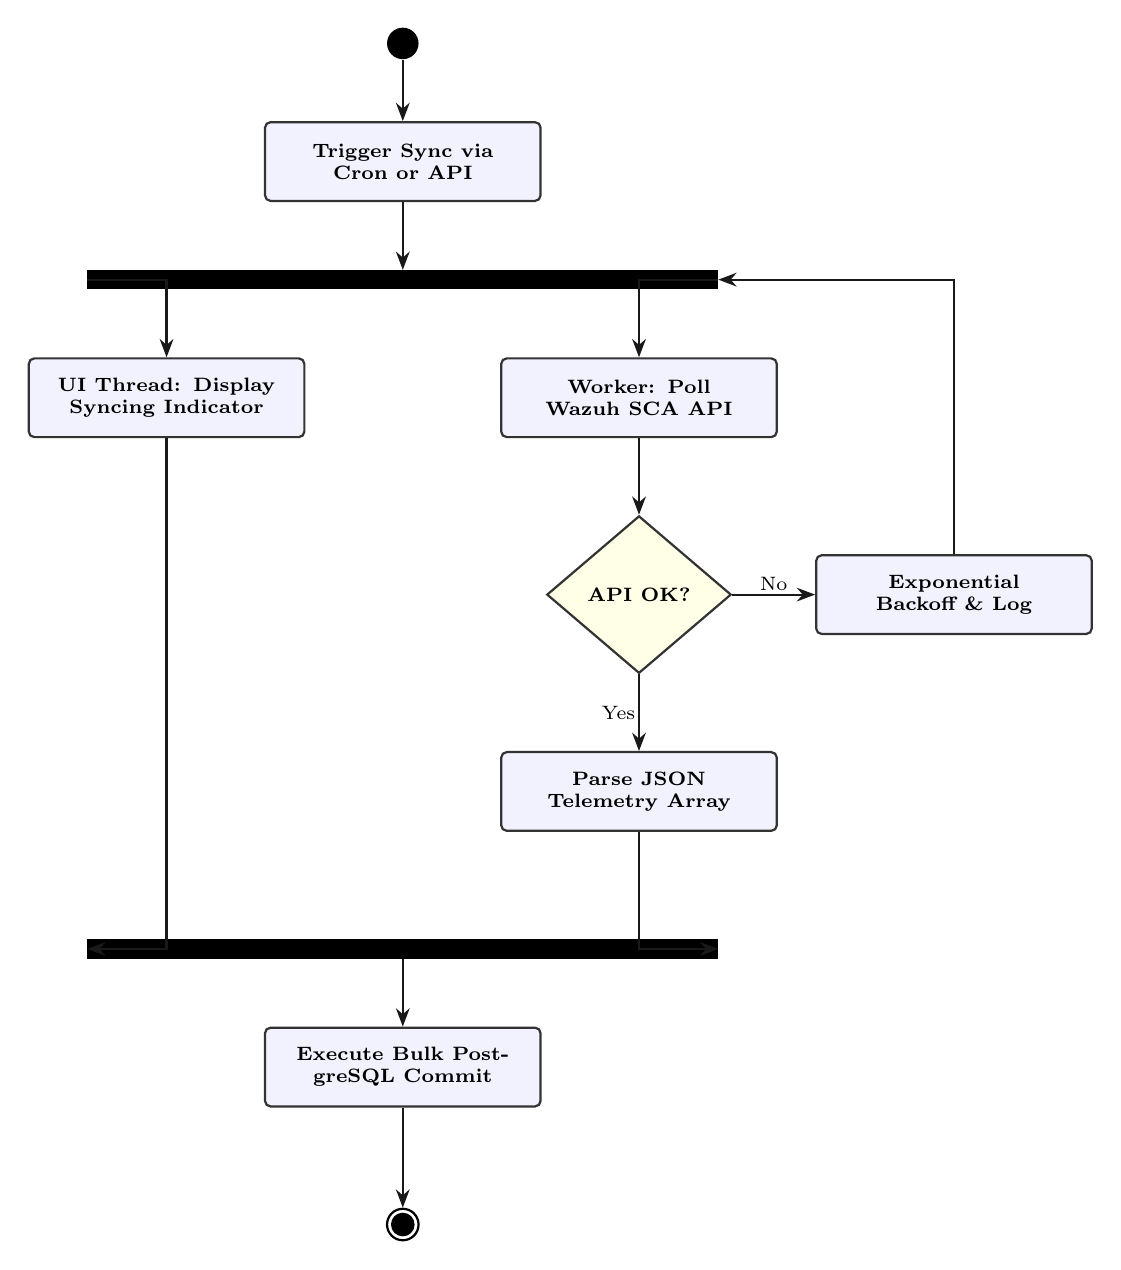
\begin{tikzpicture}[
        node distance=1.5cm,
        startstop/.style={circle, fill=black, minimum size=0.4cm},
        end/.style={circle, draw=black, thick, minimum size=0.4cm, path picture={\fill[black] (path picture bounding box.center) circle (0.15cm);}},
        activity/.style={rectangle, draw=black!80, thick, fill=blue!5, minimum width=3.5cm, minimum height=1cm, align=center, font=\scriptsize\bfseries, rounded corners=2pt, text width=3.2cm},
        decision/.style={diamond, draw=black!80, thick, fill=yellow!10, minimum width=2cm, minimum height=2cm, align=center, font=\scriptsize\bfseries, aspect=1.5, text width=1.5cm},
        fork/.style={rectangle, draw=black, fill=black, minimum width=8cm, minimum height=0.15cm},
        arrow/.style={-Stealth, thick, draw=black!90},
        label/.style={font=\scriptsize, fill=white, inner sep=1pt}
    ]
        \node[startstop] (start) at (0,0) {};
        \node[activity] (trigger) at (0,-1.5) {Trigger Sync via Cron or API};
        \node[fork] (fork1) at (0,-3) {};
        
        \node[activity] (ui) at (-3,-4.5) {UI Thread: Display Syncing Indicator};
        \node[activity] (celery) at (3,-4.5) {Worker: Poll Wazuh SCA API};
        \node[decision] (api) at (3,-7) {API OK?};
        \node[activity] (retry) at (7,-7) {Exponential Backoff \& Log};
        \node[activity] (parse) at (3,-9.5) {Parse JSON Telemetry Array};

        \node[fork] (join1) at (0,-11.5) {};
        \node[activity] (commit) at (0,-13) {Execute Bulk PostgreSQL Commit};
        \node[end] (end) at (0,-15) {};

        \draw[arrow] (start) -- (trigger);
        \draw[arrow] (trigger) -- (fork1);
        \draw[arrow] (fork1) -| (ui);
        \draw[arrow] (fork1) -| (celery);
        \draw[arrow] (celery) -- (api);
        \draw[arrow] (api) -- (retry) node[midway, above, label] {No};
        \draw[arrow] (retry) |- (fork1);
        \draw[arrow] (api) -- (parse) node[midway, left, label] {Yes};
        
        \draw[arrow] (ui) |- (join1);
        \draw[arrow] (parse) |- (join1);
        \draw[arrow] (join1) -- (commit);
        \draw[arrow] (commit) -- (end);
    \end{tikzpicture}
    }
    \caption{Activity Diagram: Parallel Asynchronous Telemetry Ingestion}
    \label{fig:activity_sync}
\end{figure}

\subsubsection{Compliance State Evaluation}
The mapping of technical alerts to policies like ISO 27001 is shown in Figure \ref{fig:activity_eval}. The system uses a worst-case priority algorithm; if a technical check fails on a single node, the corresponding governance control is marked as non-compliant. This evaluation continues until all policies are processed.

\begin{figure}[H]
    \centering
    \resizebox{0.75\textwidth}{!}{
    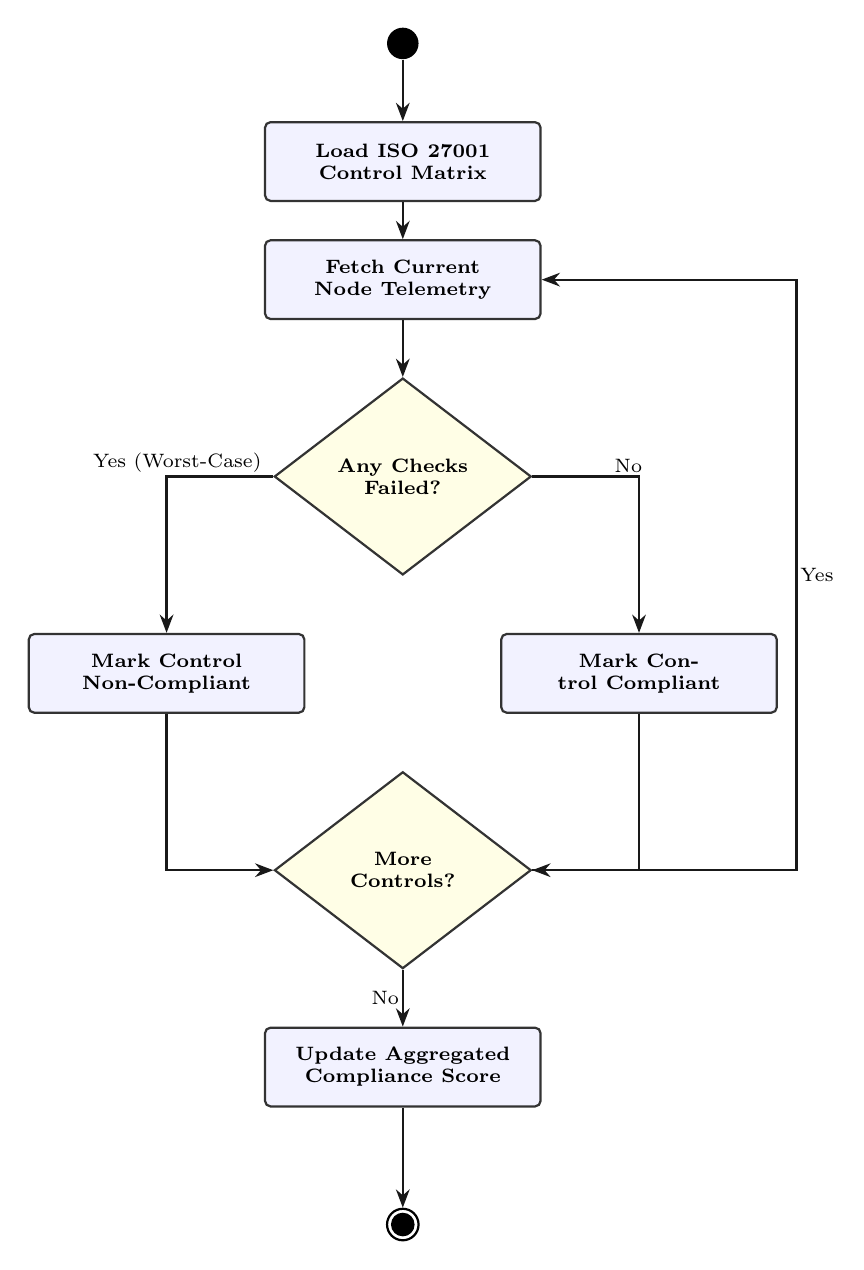
\begin{tikzpicture}[
        node distance=1.5cm,
        startstop/.style={circle, fill=black, minimum size=0.4cm},
        end/.style={circle, draw=black, thick, minimum size=0.4cm, path picture={\fill[black] (path picture bounding box.center) circle (0.15cm);}},
        activity/.style={rectangle, draw=black!80, thick, fill=blue!5, minimum width=3.5cm, minimum height=1cm, align=center, font=\scriptsize\bfseries, rounded corners=2pt, text width=3.2cm},
        decision/.style={diamond, draw=black!80, thick, fill=yellow!10, minimum width=2.5cm, minimum height=2.5cm, align=center, font=\scriptsize\bfseries, aspect=1.5, text width=2cm},
        arrow/.style={-Stealth, thick, draw=black!90},
        label/.style={font=\scriptsize, fill=white, inner sep=1pt}
    ]
        \node[startstop] (start) at (0,0) {};
        \node[activity] (load) at (0,-1.5) {Load ISO 27001 Control Matrix};
        \node[activity] (fetch) at (0,-3) {Fetch Current Node Telemetry};
        \node[decision] (check) at (0,-5.5) {Any Checks Failed?};
        \node[activity] (fail) at (-3,-8) {Mark Control Non-Compliant};
        \node[activity] (pass) at (3,-8) {Mark Control Compliant};
        \node[decision] (more) at (0,-10.5) {More Controls?};
        \node[activity] (render) at (0,-13) {Update Aggregated Compliance Score};
        \node[end] (end) at (0,-15) {};

        \draw[arrow] (start) -- (load);
        \draw[arrow] (load) -- (fetch);
        \draw[arrow] (fetch) -- (check);
        \draw[arrow] (check) -| (fail) node[pos=0.45, above, label] {Yes (Worst-Case)};
        \draw[arrow] (check) -| (pass) node[pos=0.45, above, label] {No};
        \draw[arrow] (fail) |- (more);
        \draw[arrow] (pass) |- (more);
        \draw[arrow] (more) -- (render) node[midway, left, label] {No};
        \draw[arrow] (more) -- ++(5,0) |- (fetch) node[pos=0.25, right, label] {Yes};
        \draw[arrow] (render) -- (end);
    \end{tikzpicture}
    }
    \caption{Activity Diagram: Iterative Compliance Evaluation and Worst-Case Priority}
    \label{fig:activity_eval}
\end{figure}

\subsubsection{Audit Report Generation}
The audit report generation process is automated, as shown in Figure \ref{fig:activity_report}. When a user selects a framework, the backend aggregates relevant database records. This data is injected into an HTML template, and a PDF is generated on the server for delivery to the client.

\begin{figure}[H]
    \centering
    \resizebox{0.6\textwidth}{!}{
    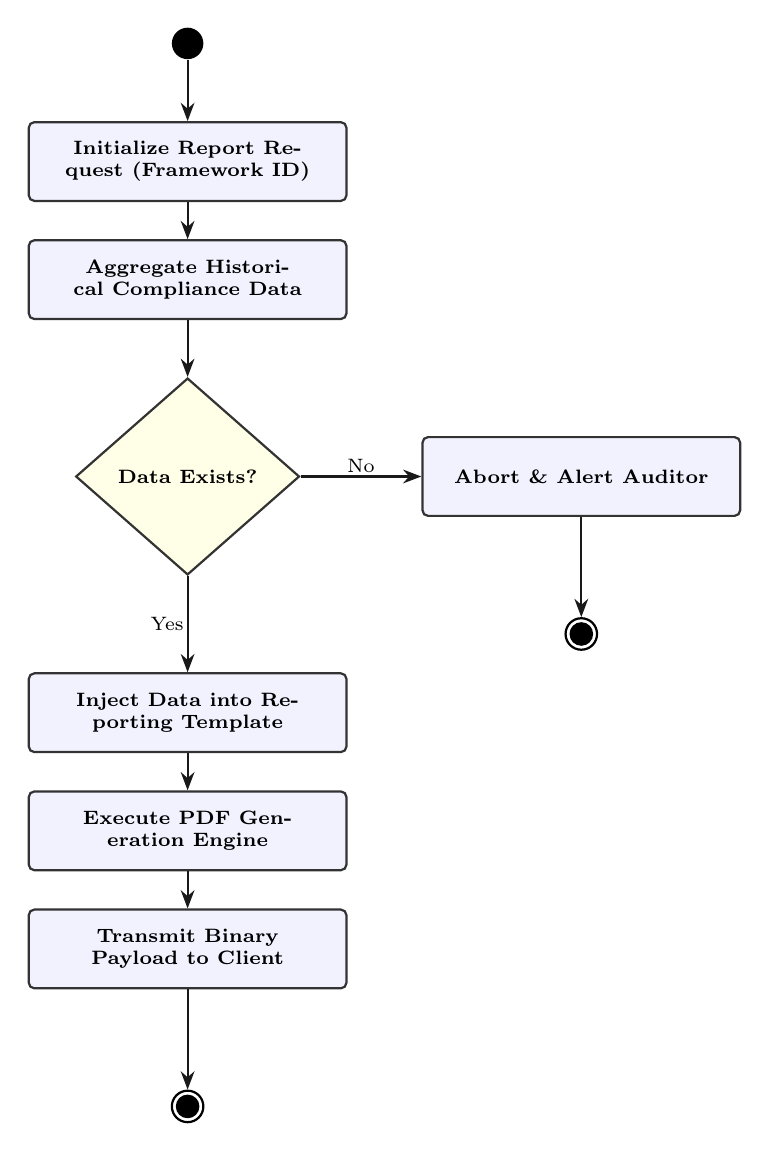
\begin{tikzpicture}[
        node distance=1.5cm,
        startstop/.style={circle, fill=black, minimum size=0.4cm},
        end/.style={circle, draw=black, thick, minimum size=0.4cm, path picture={\fill[black] (path picture bounding box.center) circle (0.15cm);}},
        activity/.style={rectangle, draw=black!80, thick, fill=blue!5, minimum width=4cm, minimum height=1cm, align=center, font=\scriptsize\bfseries, rounded corners=2pt, text width=3.8cm},
        decision/.style={diamond, draw=black!80, thick, fill=yellow!10, minimum width=2.5cm, minimum height=2.5cm, align=center, font=\scriptsize\bfseries, aspect=1.5, text width=2cm},
        arrow/.style={-Stealth, thick, draw=black!90},
        label/.style={font=\scriptsize, fill=white, inner sep=1pt}
    ]
        \node[startstop] (start) at (0,0) {};
        \node[activity] (request) at (0,-1.5) {Initialize Report Request (Framework ID)};
        \node[activity] (query) at (0,-3) {Aggregate Historical Compliance Data};
        \node[decision] (data) at (0,-5.5) {Data Exists?};
        \node[activity] (error) at (5,-5.5) {Abort \& Alert Auditor};
        \node[activity] (template) at (0,-8.5) {Inject Data into Reporting Template};
        \node[activity] (pdf) at (0,-10) {Execute PDF Generation Engine};
        \node[activity] (download) at (0,-11.5) {Transmit Binary Payload to Client};
        \node[end] (end1) at (5,-7.5) {};
        \node[end] (end2) at (0,-13.5) {};

        \draw[arrow] (start) -- (request);
        \draw[arrow] (request) -- (query);
        \draw[arrow] (query) -- (data);
        \draw[arrow] (data) -- (error) node[midway, above, label] {No};
        \draw[arrow] (error) -- (end1);
        \draw[arrow] (data) -- (template) node[midway, left, label] {Yes};
        \draw[arrow] (template) -- (pdf);
        \draw[arrow] (pdf) -- (download);
        \draw[arrow] (download) -- (end2);
    \end{tikzpicture}
    }
    \caption{Activity Diagram: Automated PDF Audit Report Generation}
    \label{fig:activity_report}
\end{figure}


\subsubsection{Framework Rule Mapping and Validation}
Administrators map Wazuh rules to framework controls as shown in Figure \ref{fig:activity_mapping}. Before saving the mapping, the system queries the SIEM API to verify the rule ID. If valid, the system checks for existing mappings in the database. This validation prevents accidental overwriting of existing configurations.

\begin{figure}[H]
    \centering
    \resizebox{0.8\textwidth}{!}{
    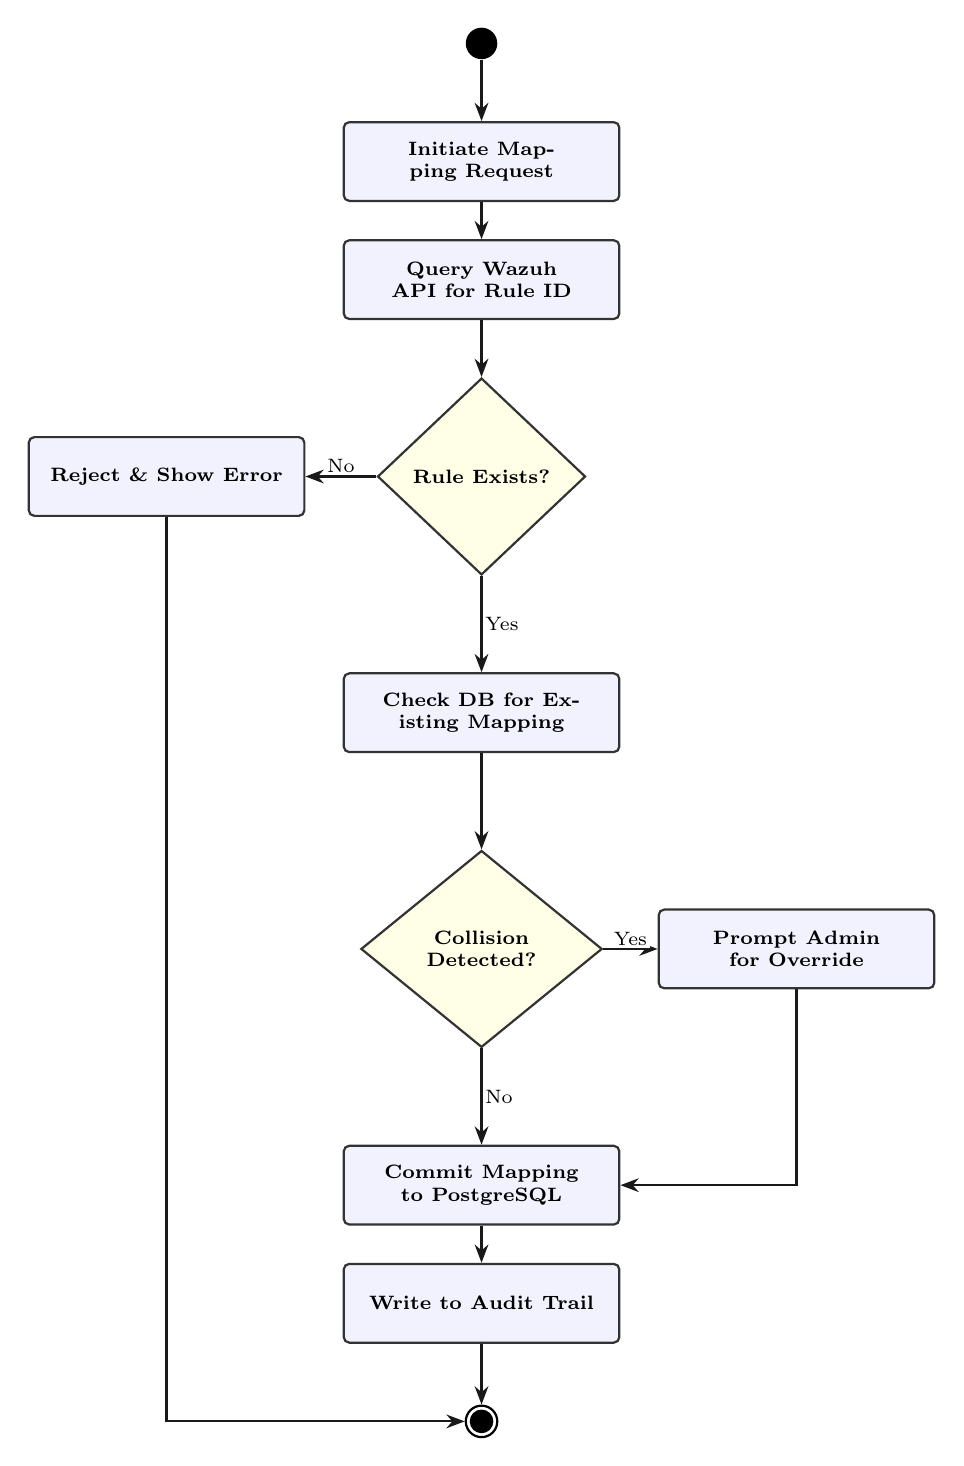
\begin{tikzpicture}[
        node distance=1.5cm,
        startstop/.style={circle, fill=black, minimum size=0.4cm},
        end/.style={circle, draw=black, thick, minimum size=0.4cm, path picture={\fill[black] (path picture bounding box.center) circle (0.15cm);}},
        activity/.style={rectangle, draw=black!80, thick, fill=blue!5, minimum width=3.5cm, minimum height=1cm, align=center, font=\scriptsize\bfseries, rounded corners=2pt, text width=3.2cm},
        decision/.style={diamond, draw=black!80, thick, fill=yellow!10, minimum width=2.5cm, minimum height=2.5cm, align=center, font=\scriptsize\bfseries, aspect=1.5, text width=1.8cm},
        arrow/.style={-Stealth, thick, draw=black!90},
        label/.style={font=\scriptsize, fill=white, inner sep=1pt}
    ]
        \node[startstop] (start) at (0,0) {};
        \node[activity] (init) at (0,-1.5) {Initiate Mapping Request};
        \node[activity] (api) at (0,-3) {Query Wazuh API for Rule ID};
        \node[decision] (exists) at (0,-5.5) {Rule Exists?};
        \node[activity] (error1) at (-4,-5.5) {Reject \& Show Error};
        \node[activity] (checkdb) at (0,-8.5) {Check DB for Existing Mapping};
        \node[decision] (collision) at (0,-11.5) {Collision Detected?};
        \node[activity] (override) at (4,-11.5) {Prompt Admin for Override};
        \node[activity] (commit) at (0,-14.5) {Commit Mapping to PostgreSQL};
        \node[activity] (audit) at (0,-16) {Write to Audit Trail};
        \node[end] (end) at (0,-17.5) {};

        \draw[arrow] (start) -- (init);
        \draw[arrow] (init) -- (api);
        \draw[arrow] (api) -- (exists);
        \draw[arrow] (exists) -- (error1) node[midway, above, label] {No};
        \draw[arrow] (exists) -- (checkdb) node[midway, right, label] {Yes};
        \draw[arrow] (checkdb) -- (collision);
        \draw[arrow] (collision) -- (override) node[midway, above, label] {Yes};
        \draw[arrow] (override) |- (commit);
        \draw[arrow] (collision) -- (commit) node[midway, right, label] {No};
        \draw[arrow] (commit) -- (audit);
        \draw[arrow] (audit) -- (end);
        \draw[arrow] (error1) |- (end);
    \end{tikzpicture}
    }
    \caption{Activity Diagram: Framework Rule Mapping and API Validation}
    \label{fig:activity_mapping}
\end{figure}

\subsubsection{Real-Time Alerting and Notification}
The platform includes an alerting pipeline as shown in Figure \ref{fig:activity_alerting}. When a compliance check fails, the engine evaluates its severity. Minor issues are recorded in the database logs, while critical failures trigger automated notifications via email and webhooks to auditors.

\begin{figure}[H]
    \centering
    \resizebox{0.8\textwidth}{!}{
    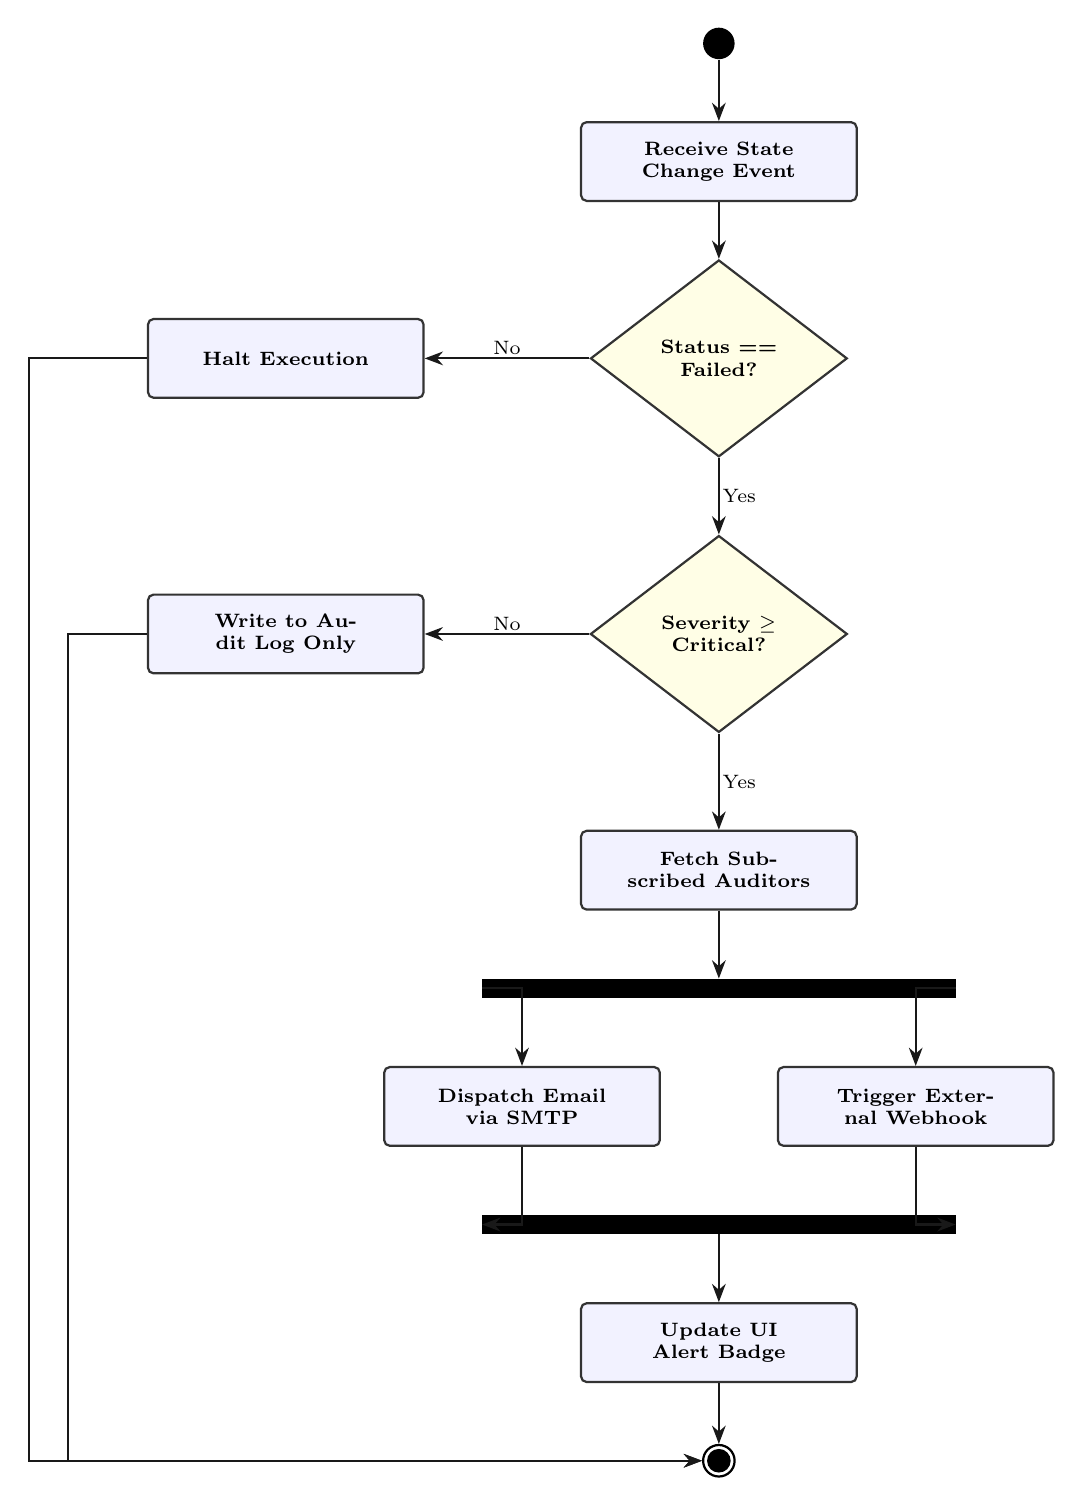
\begin{tikzpicture}[
        node distance=1.5cm,
        startstop/.style={circle, fill=black, minimum size=0.4cm},
        end/.style={circle, draw=black, thick, minimum size=0.4cm, path picture={\fill[black] (path picture bounding box.center) circle (0.15cm);}},
        activity/.style={rectangle, draw=black!80, thick, fill=blue!5, minimum width=3.5cm, minimum height=1cm, align=center, font=\scriptsize\bfseries, rounded corners=2pt, text width=3.2cm},
        decision/.style={diamond, draw=black!80, thick, fill=yellow!10, minimum width=2.5cm, minimum height=2.5cm, align=center, font=\scriptsize\bfseries, aspect=1.5, text width=2cm},
        fork/.style={rectangle, draw=black, fill=black, minimum width=6cm, minimum height=0.15cm},
        arrow/.style={-Stealth, thick, draw=black!90},
        label/.style={font=\scriptsize, fill=white, inner sep=1pt}
    ]
        \node[startstop] (start) at (0,0) {};
        \node[activity] (event) at (0,-1.5) {Receive State Change Event};
        \node[decision] (failed) at (0,-4) {Status == Failed?};
        \node[activity] (ignore) at (-5.5,-4) {Halt Execution};
        \node[decision] (severity) at (0,-7.5) {Severity $\ge$ Critical?};
        \node[activity] (log) at (-5.5,-7.5) {Write to Audit Log Only};
        \node[activity] (fetch) at (0,-10.5) {Fetch Subscribed Auditors};
        
        \node[fork] (fork1) at (0,-12) {};
        \node[activity] (email) at (-2.5,-13.5) {Dispatch Email via SMTP};
        \node[activity] (webhook) at (2.5,-13.5) {Trigger External Webhook};
        \node[fork] (join1) at (0,-15) {};
        
        \node[activity] (badge) at (0,-16.5) {Update UI Alert Badge};
        \node[end] (end) at (0,-18) {};

        \draw[arrow] (start) -- (event);
        \draw[arrow] (event) -- (failed);
        \draw[arrow] (failed) -- (ignore) node[midway, above, label] {No};
        \draw[arrow] (failed) -- (severity) node[midway, right, label] {Yes};
        \draw[arrow] (severity) -- (log) node[midway, above, label] {No};
        \draw[arrow] (severity) -- (fetch) node[midway, right, label] {Yes};
        \draw[arrow] (fetch) -- (fork1);
        \draw[arrow] (fork1) -| (email);
        \draw[arrow] (fork1) -| (webhook);
        \draw[arrow] (email) |- (join1);
        \draw[arrow] (webhook) |- (join1);
        \draw[arrow] (join1) -- (badge);
        \draw[arrow] (badge) -- (end);
        \draw[arrow] (ignore.west) -- ++(-1.5,0) |- (end);
        \draw[arrow] (log.west) -- ++(-1,0) |- (end);
    \end{tikzpicture}
    }
    \caption{Activity Diagram: Real-Time Alerting and Notification Fan-out}
    \label{fig:activity_alerting}
\end{figure}

\subsection{System Sequence Diagrams}
The sequence diagrams below trace the linear interactions between internal system components for each use case. Each diagram is identified by an SD-XX-Y code that maps directly to the parent UC-XX use case.

\subsubsection{SD-01: User Authentication}
The authentication sequence covers both the success and failure paths for UC-01. A valid credential submission results in JWT issuance, while an invalid submission terminates with an HTTP 401 response. These two paths are documented as SD-01-1 and SD-01-2 respectively.

Figure \ref{fig:sd_01_1} traces the success path. The client submits credentials via POST /login, the IAM module verifies the password hash against the database, signs a JWT, and returns it to the client.

\begin{figure}[H]
    \centering
    \resizebox{0.95\textwidth}{!}{
    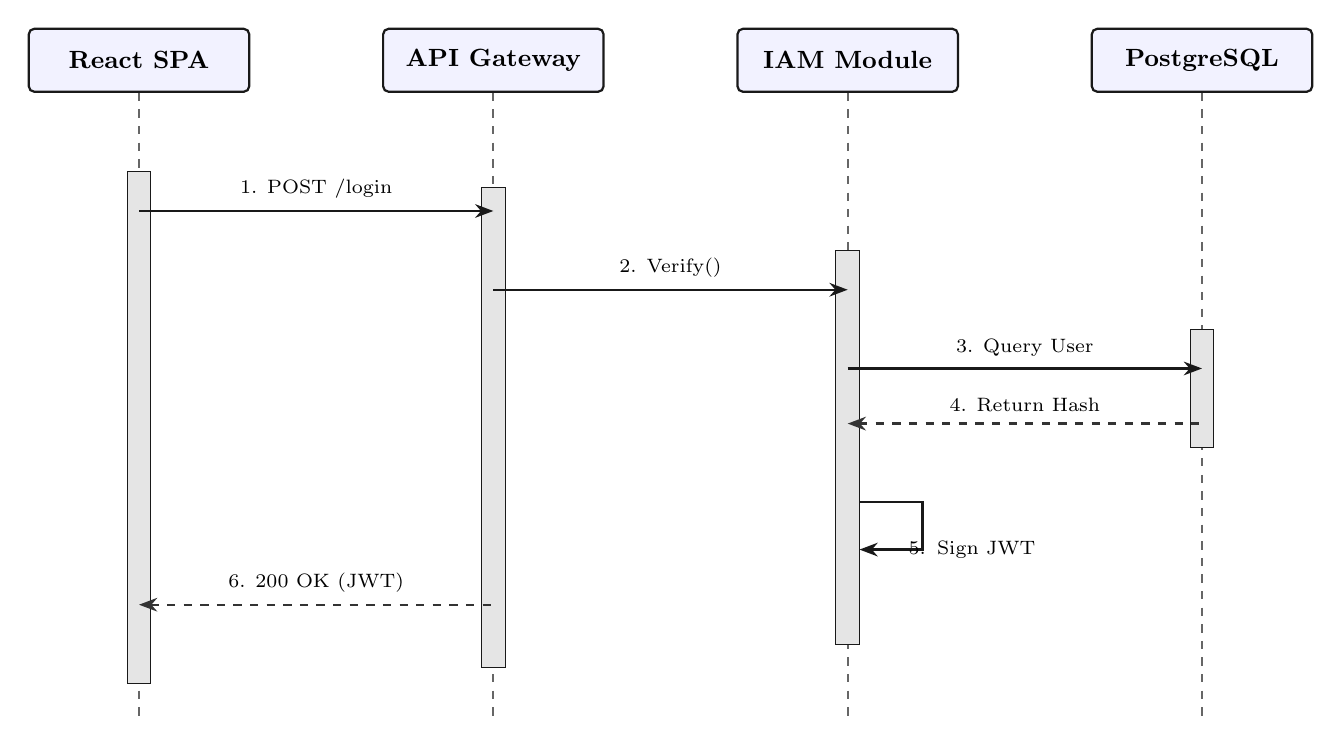
\begin{tikzpicture}[
        node distance=2cm,
        inst/.style={rectangle, draw=black!90, thick, fill=blue!5, minimum width=2.8cm, minimum height=0.8cm, font=\small\bfseries, rounded corners=2pt},
        act/.style={rectangle, draw=black!90, fill=gray!20, minimum width=0.3cm},
        msg/.style={-Stealth, thick, draw=black!90},
        reply/.style={Stealth-, thick, dashed, draw=black!80},
        label/.style={font=\scriptsize, inner sep=2pt}
    ]
        \node[inst] (client) at (0, 0) {React SPA};
        \node[inst] (api) at (4.5, 0) {API Gateway};
        \node[inst] (iam) at (9, 0) {IAM Module};
        \node[inst] (db) at (13.5, 0) {PostgreSQL};
        \draw[dashed, draw=black!60, thick] (client.south) -- ++(0, -8);
        \draw[dashed, draw=black!60, thick] (api.south) -- ++(0, -8);
        \draw[dashed, draw=black!60, thick] (iam.south) -- ++(0, -8);
        \draw[dashed, draw=black!60, thick] (db.south) -- ++(0, -8);
        \draw[act] ([xshift=-0.15cm, yshift=-1cm]client.south) rectangle ([xshift=0.15cm, yshift=-7.5cm]client.south);
        \draw[act] ([xshift=-0.15cm, yshift=-1.2cm]api.south) rectangle ([xshift=0.15cm, yshift=-7.3cm]api.south);
        \draw[act] ([xshift=-0.15cm, yshift=-2cm]iam.south) rectangle ([xshift=0.15cm, yshift=-7cm]iam.south);
        \draw[act] ([xshift=-0.15cm, yshift=-3cm]db.south) rectangle ([xshift=0.15cm, yshift=-4.5cm]db.south);
        \draw[msg] ([yshift=-1.5cm]client.south) -- ([yshift=-1.5cm]api.south) node[midway, above=2pt, label] {1. POST /login};
        \draw[msg] ([yshift=-2.5cm]api.south) -- ([yshift=-2.5cm]iam.south) node[midway, above=2pt, label] {2. Verify()};
        \draw[msg] ([yshift=-3.5cm]iam.south) -- ([yshift=-3.5cm]db.south) node[midway, above=2pt, label] {3. Query User};
        \draw[reply] ([yshift=-4.2cm]iam.south) -- ([yshift=-4.2cm]db.south) node[midway, above=2pt, label] {4. Return Hash};
        \draw[msg] ([yshift=-5.2cm]iam.south) ++(0.15cm,0) -- ++(0.8,0) -- ++(0,-0.6) -- ++(-0.8,0) node[midway, right=4pt, label, text width=2cm] {5. Sign JWT};
        \draw[reply] ([yshift=-6.5cm]client.south) -- ([yshift=-6.5cm]api.south) node[midway, above=2pt, label] {6. 200 OK (JWT)};
    \end{tikzpicture}
    }
    \caption{SD-01-1: Valid Authentication Flow}
    \label{fig:sd_01_1}
\end{figure}

Figure \ref{fig:sd_01_2} traces the failure path. The submitted password hash does not match, and the system returns an HTTP 401 response without issuing any tokens.

\begin{figure}[H]
    \centering
    \resizebox{0.85\textwidth}{!}{
    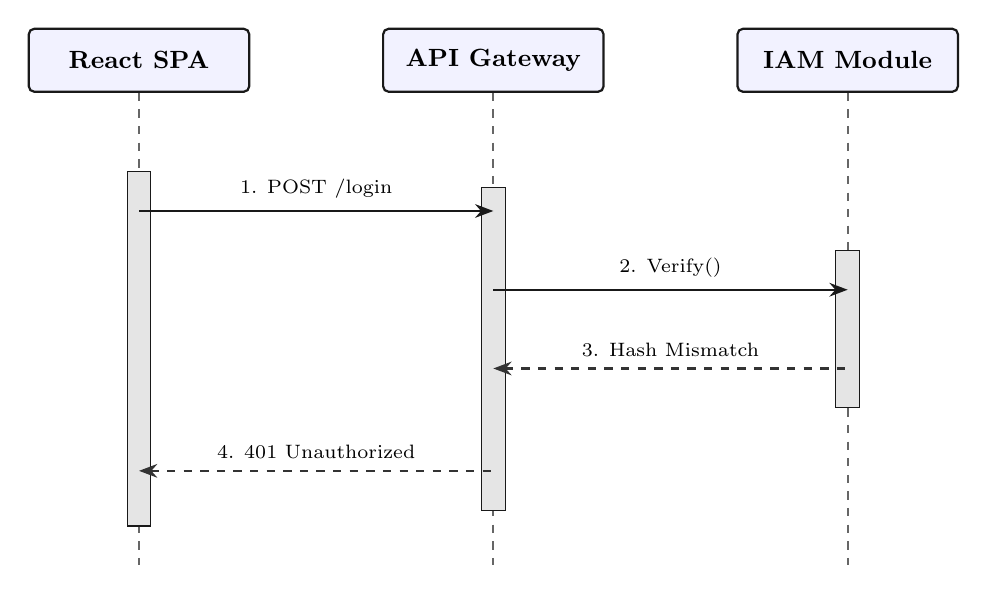
\begin{tikzpicture}[
        node distance=2cm,
        inst/.style={rectangle, draw=black!90, thick, fill=blue!5, minimum width=2.8cm, minimum height=0.8cm, font=\small\bfseries, rounded corners=2pt},
        act/.style={rectangle, draw=black!90, fill=gray!20, minimum width=0.3cm},
        msg/.style={-Stealth, thick, draw=black!90},
        reply/.style={Stealth-, thick, dashed, draw=black!80},
        label/.style={font=\scriptsize, inner sep=2pt}
    ]
        \node[inst] (client) at (0, 0) {React SPA};
        \node[inst] (api) at (4.5, 0) {API Gateway};
        \node[inst] (iam) at (9, 0) {IAM Module};
        \draw[dashed, draw=black!60, thick] (client.south) -- ++(0, -6);
        \draw[dashed, draw=black!60, thick] (api.south) -- ++(0, -6);
        \draw[dashed, draw=black!60, thick] (iam.south) -- ++(0, -6);
        \draw[act] ([xshift=-0.15cm, yshift=-1cm]client.south) rectangle ([xshift=0.15cm, yshift=-5.5cm]client.south);
        \draw[act] ([xshift=-0.15cm, yshift=-1.2cm]api.south) rectangle ([xshift=0.15cm, yshift=-5.3cm]api.south);
        \draw[act] ([xshift=-0.15cm, yshift=-2cm]iam.south) rectangle ([xshift=0.15cm, yshift=-4cm]iam.south);
        \draw[msg] ([yshift=-1.5cm]client.south) -- ([yshift=-1.5cm]api.south) node[midway, above=2pt, label] {1. POST /login};
        \draw[msg] ([yshift=-2.5cm]api.south) -- ([yshift=-2.5cm]iam.south) node[midway, above=2pt, label] {2. Verify()};
        \draw[reply] ([yshift=-3.5cm]api.south) -- ([yshift=-3.5cm]iam.south) node[midway, above=2pt, label] {3. Hash Mismatch};
        \draw[reply] ([yshift=-4.8cm]client.south) -- ([yshift=-4.8cm]api.south) node[midway, above=2pt, label] {4. 401 Unauthorized};
    \end{tikzpicture}
    }
    \caption{SD-01-2: Invalid Authentication Flow}
    \label{fig:sd_01_2}
\end{figure}

\subsubsection{SD-02: Manage Wazuh Telemetry Synchronization}
This sequence traces UC-02, the telemetry synchronization pipeline. The Django API dispatches the task to a Celery worker, which polls the Wazuh SIEM, maps the returned rules to framework controls, and commits the resolved states to PostgreSQL.

Figure \ref{fig:sd_02_1} documents the linear success path for the synchronization operation.

\begin{figure}[H]
    \centering
    \resizebox{0.95\textwidth}{!}{
    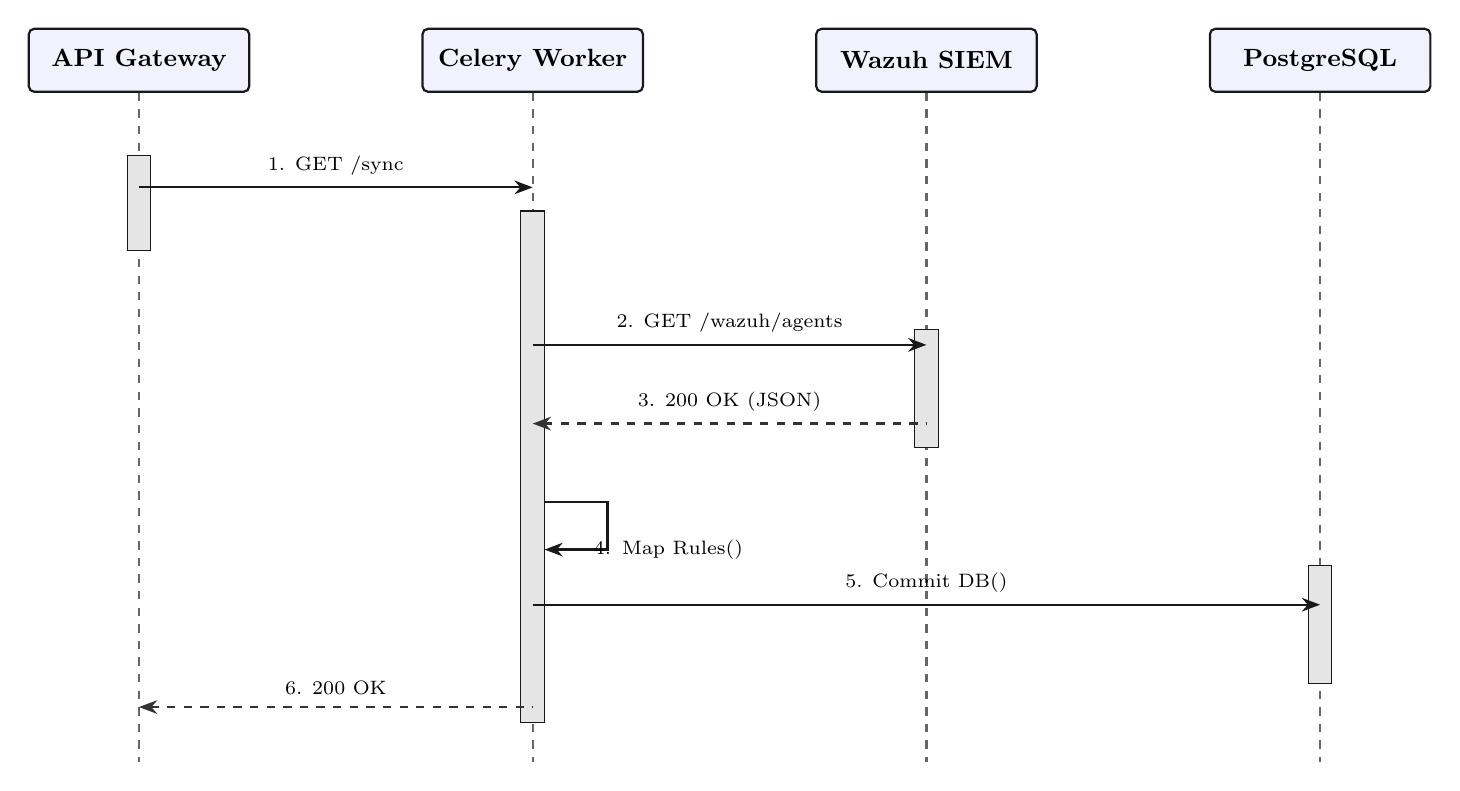
\begin{tikzpicture}[
        node distance=2cm,
        inst/.style={rectangle, draw=black!90, thick, fill=blue!5, minimum width=2.8cm, minimum height=0.8cm, font=\small\bfseries, rounded corners=2pt},
        act/.style={rectangle, draw=black!90, fill=gray!20, minimum width=0.3cm},
        msg/.style={-Stealth, thick, draw=black!90},
        reply/.style={Stealth-, thick, dashed, draw=black!80},
        label/.style={font=\scriptsize, inner sep=2pt}
    ]
        \node[inst] (api) at (0, 0) {API Gateway};
        \node[inst] (celery) at (5, 0) {Celery Worker};
        \node[inst] (wazuh) at (10, 0) {Wazuh SIEM};
        \node[inst] (db) at (15, 0) {PostgreSQL};
        \draw[dashed, draw=black!60, thick] (api.south) -- ++(0, -8.5);
        \draw[dashed, draw=black!60, thick] (celery.south) -- ++(0, -8.5);
        \draw[dashed, draw=black!60, thick] (wazuh.south) -- ++(0, -8.5);
        \draw[dashed, draw=black!60, thick] (db.south) -- ++(0, -8.5);
        \draw[act] ([xshift=-0.15cm, yshift=-0.8cm]api.south) rectangle ([xshift=0.15cm, yshift=-2cm]api.south);
        \draw[act] ([xshift=-0.15cm, yshift=-1.5cm]celery.south) rectangle ([xshift=0.15cm, yshift=-8cm]celery.south);
        \draw[act] ([xshift=-0.15cm, yshift=-3cm]wazuh.south) rectangle ([xshift=0.15cm, yshift=-4.5cm]wazuh.south);
        \draw[act] ([xshift=-0.15cm, yshift=-6cm]db.south) rectangle ([xshift=0.15cm, yshift=-7.5cm]db.south);
        \draw[msg] ([yshift=-1.2cm]api.south) -- ([yshift=-1.2cm]celery.south) node[midway, above=2pt, label] {1. GET /sync};
        \draw[msg] ([yshift=-3.2cm]celery.south) -- ([yshift=-3.2cm]wazuh.south) node[midway, above=2pt, label] {2. GET /wazuh/agents};
        \draw[reply] ([yshift=-4.2cm]celery.south) -- ([yshift=-4.2cm]wazuh.south) node[midway, above=2pt, label] {3. 200 OK (JSON)};
        \draw[msg] ([yshift=-5.2cm]celery.south) ++(0.15cm,0) -- ++(0.8,0) -- ++(0,-0.6) -- ++(-0.8,0) node[midway, right=4pt, label, text width=2cm] {4. Map Rules()};
        \draw[msg] ([yshift=-6.5cm]celery.south) -- ([yshift=-6.5cm]db.south) node[midway, above=2pt, label] {5. Commit DB()};
        \draw[reply] ([yshift=-7.8cm]api.south) -- ([yshift=-7.8cm]celery.south) node[midway, above=2pt, label] {6. 200 OK};
    \end{tikzpicture}
    }
    \caption{SD-02-1: Telemetry Synchronization Success}
    \label{fig:sd_02_1}
\end{figure}

\subsubsection{SD-03: Map Framework Controls to Wazuh Rules}
This sequence covers UC-03, the framework-to-rule mapping operation. SD-03-1 documents the success path where a new mapping is validated and persisted. SD-03-2 documents the collision path where the backend detects and rejects a duplicate entry.

Figure \ref{fig:sd_03_1} traces the success path for creating a new control mapping.

\begin{figure}[H]
    \centering
    \resizebox{0.8\textwidth}{!}{
    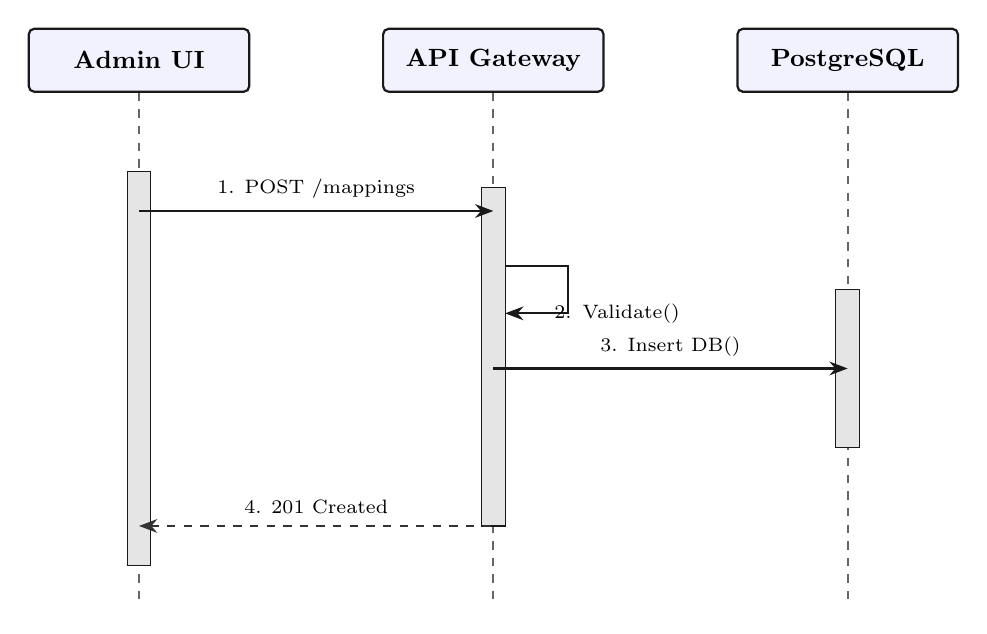
\begin{tikzpicture}[
        node distance=2cm,
        inst/.style={rectangle, draw=black!90, thick, fill=blue!5, minimum width=2.8cm, minimum height=0.8cm, font=\small\bfseries, rounded corners=2pt},
        act/.style={rectangle, draw=black!90, fill=gray!20, minimum width=0.3cm},
        msg/.style={-Stealth, thick, draw=black!90},
        reply/.style={Stealth-, thick, dashed, draw=black!80},
        label/.style={font=\scriptsize, inner sep=2pt}
    ]
        \node[inst] (client) at (0, 0) {Admin UI};
        \node[inst] (api) at (4.5, 0) {API Gateway};
        \node[inst] (db) at (9, 0) {PostgreSQL};
        \draw[dashed, draw=black!60, thick] (client.south) -- ++(0, -6.5);
        \draw[dashed, draw=black!60, thick] (api.south) -- ++(0, -6.5);
        \draw[dashed, draw=black!60, thick] (db.south) -- ++(0, -6.5);
        \draw[act] ([xshift=-0.15cm, yshift=-1cm]client.south) rectangle ([xshift=0.15cm, yshift=-6cm]client.south);
        \draw[act] ([xshift=-0.15cm, yshift=-1.2cm]api.south) rectangle ([xshift=0.15cm, yshift=-5.5cm]api.south);
        \draw[act] ([xshift=-0.15cm, yshift=-2.5cm]db.south) rectangle ([xshift=0.15cm, yshift=-4.5cm]db.south);
        \draw[msg] ([yshift=-1.5cm]client.south) -- ([yshift=-1.5cm]api.south) node[midway, above=2pt, label] {1. POST /mappings};
        \draw[msg] ([yshift=-2.2cm]api.south) ++(0.15cm,0) -- ++(0.8,0) -- ++(0,-0.6) -- ++(-0.8,0) node[midway, right=4pt, label, text width=2cm] {2. Validate()};
        \draw[msg] ([yshift=-3.5cm]api.south) -- ([yshift=-3.5cm]db.south) node[midway, above=2pt, label] {3. Insert DB()};
        \draw[reply] ([yshift=-5.5cm]client.south) -- ([yshift=-5.5cm]api.south) node[midway, above=2pt, label] {4. 201 Created};
    \end{tikzpicture}
    }
    \caption{SD-03-1: Map Controls Success}
    \label{fig:sd_03_1}
\end{figure}

Figure \ref{fig:sd_03_2} traces the collision path where the backend detects a duplicate mapping and rejects it with HTTP 400.

\begin{figure}[H]
    \centering
    \resizebox{0.8\textwidth}{!}{
    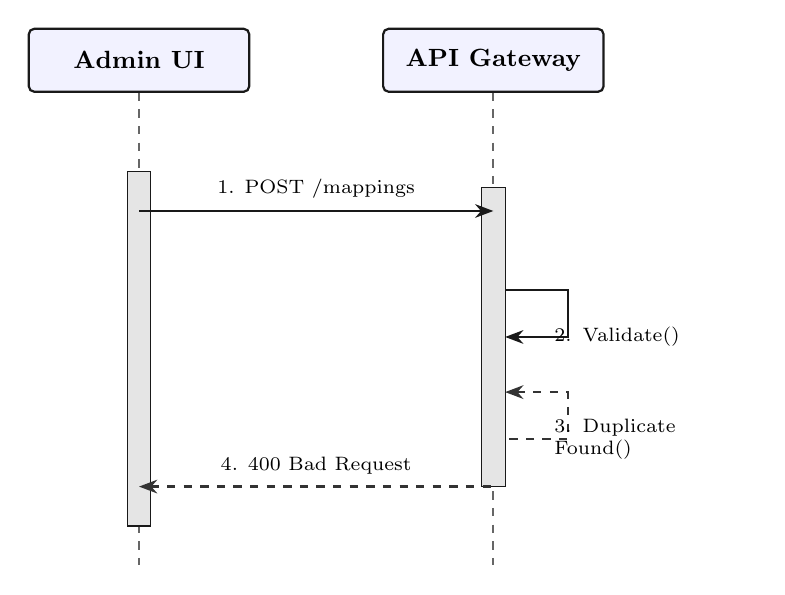
\begin{tikzpicture}[
        node distance=2cm,
        inst/.style={rectangle, draw=black!90, thick, fill=blue!5, minimum width=2.8cm, minimum height=0.8cm, font=\small\bfseries, rounded corners=2pt},
        act/.style={rectangle, draw=black!90, fill=gray!20, minimum width=0.3cm},
        msg/.style={-Stealth, thick, draw=black!90},
        reply/.style={Stealth-, thick, dashed, draw=black!80},
        label/.style={font=\scriptsize, inner sep=2pt}
    ]
        \node[inst] (client) at (0, 0) {Admin UI};
        \node[inst] (api) at (4.5, 0) {API Gateway};
        \draw[dashed, draw=black!60, thick] (client.south) -- ++(0, -6);
        \draw[dashed, draw=black!60, thick] (api.south) -- ++(0, -6);
        \draw[act] ([xshift=-0.15cm, yshift=-1cm]client.south) rectangle ([xshift=0.15cm, yshift=-5.5cm]client.south);
        \draw[act] ([xshift=-0.15cm, yshift=-1.2cm]api.south) rectangle ([xshift=0.15cm, yshift=-5cm]api.south);
        \draw[msg] ([yshift=-1.5cm]client.south) -- ([yshift=-1.5cm]api.south) node[midway, above=2pt, label] {1. POST /mappings};
        \draw[msg] ([yshift=-2.5cm]api.south) ++(0.15cm,0) -- ++(0.8,0) -- ++(0,-0.6) -- ++(-0.8,0) node[midway, right=4pt, label, text width=2cm] {2. Validate()};
        \draw[reply] ([yshift=-3.8cm]api.south) ++(0.15cm,0) -- ++(0.8,0) -- ++(0,-0.6) -- ++(-0.8,0) node[midway, right=4pt, label, text width=2.5cm] {3. Duplicate Found()};
        \draw[reply] ([yshift=-5cm]client.south) -- ([yshift=-5cm]api.south) node[midway, above=2pt, label] {4. 400 Bad Request};
    \end{tikzpicture}
    }
    \caption{SD-03-2: Map Collision}
    \label{fig:sd_03_2}
\end{figure}

\subsubsection{SD-04: Monitor Endpoint Compliance Status}
This sequence traces UC-04, the dashboard compliance monitoring flow. The React SPA requests the aggregated compliance metrics from the API, which queries PostgreSQL and returns the calculated data array for visualization on the dashboard gauge.

Figure \ref{fig:sd_04_1} documents the data retrieval path for the compliance dashboard.

\begin{figure}[H]
    \centering
    \resizebox{0.85\textwidth}{!}{
    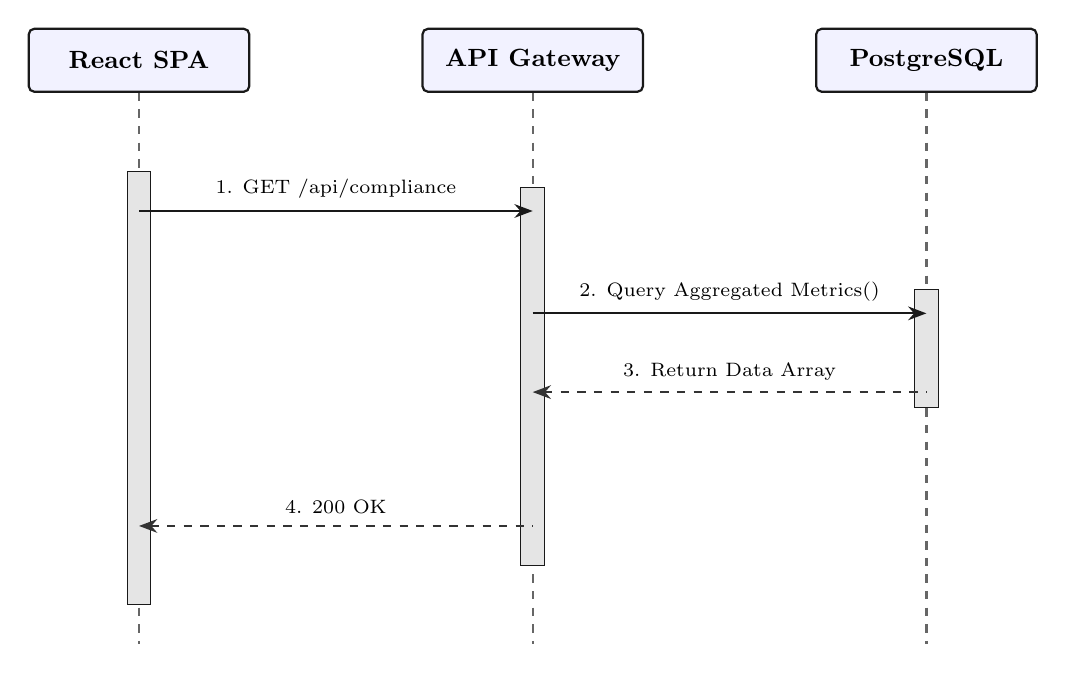
\begin{tikzpicture}[
        node distance=2cm,
        inst/.style={rectangle, draw=black!90, thick, fill=blue!5, minimum width=2.8cm, minimum height=0.8cm, font=\small\bfseries, rounded corners=2pt},
        act/.style={rectangle, draw=black!90, fill=gray!20, minimum width=0.3cm},
        msg/.style={-Stealth, thick, draw=black!90},
        reply/.style={Stealth-, thick, dashed, draw=black!80},
        label/.style={font=\scriptsize, inner sep=2pt}
    ]
        \node[inst] (client) at (0, 0) {React SPA};
        \node[inst] (api) at (5, 0) {API Gateway};
        \node[inst] (db) at (10, 0) {PostgreSQL};
        \draw[dashed, draw=black!60, thick] (client.south) -- ++(0, -7);
        \draw[dashed, draw=black!60, thick] (api.south) -- ++(0, -7);
        \draw[dashed, draw=black!60, thick] (db.south) -- ++(0, -7);
        \draw[act] ([xshift=-0.15cm, yshift=-1cm]client.south) rectangle ([xshift=0.15cm, yshift=-6.5cm]client.south);
        \draw[act] ([xshift=-0.15cm, yshift=-1.2cm]api.south) rectangle ([xshift=0.15cm, yshift=-6cm]api.south);
        \draw[act] ([xshift=-0.15cm, yshift=-2.5cm]db.south) rectangle ([xshift=0.15cm, yshift=-4cm]db.south);
        \draw[msg] ([yshift=-1.5cm]client.south) -- ([yshift=-1.5cm]api.south) node[midway, above=2pt, label] {1. GET /api/compliance};
        \draw[msg] ([yshift=-2.8cm]api.south) -- ([yshift=-2.8cm]db.south) node[midway, above=2pt, label] {2. Query Aggregated Metrics()};
        \draw[reply] ([yshift=-3.8cm]api.south) -- ([yshift=-3.8cm]db.south) node[midway, above=2pt, label] {3. Return Data Array};
        \draw[reply] ([yshift=-5.5cm]client.south) -- ([yshift=-5.5cm]api.south) node[midway, above=2pt, label] {4. 200 OK};
    \end{tikzpicture}
    }
    \caption{SD-04-1: Monitor Endpoint Compliance Status}
    \label{fig:sd_04_1}
\end{figure}

\subsubsection{SD-05: Resolve Compliance Anomalies}
This sequence traces UC-05, the anomaly remediation workflow. An administrator submits a remediation request through the UI. The API dispatches the task to a Celery worker, which updates the control status in PostgreSQL and confirms the resolution.

Figure \ref{fig:sd_05_1} documents the remediation dispatch and confirmation path.

\begin{figure}[H]
    \centering
    \resizebox{0.9\textwidth}{!}{
    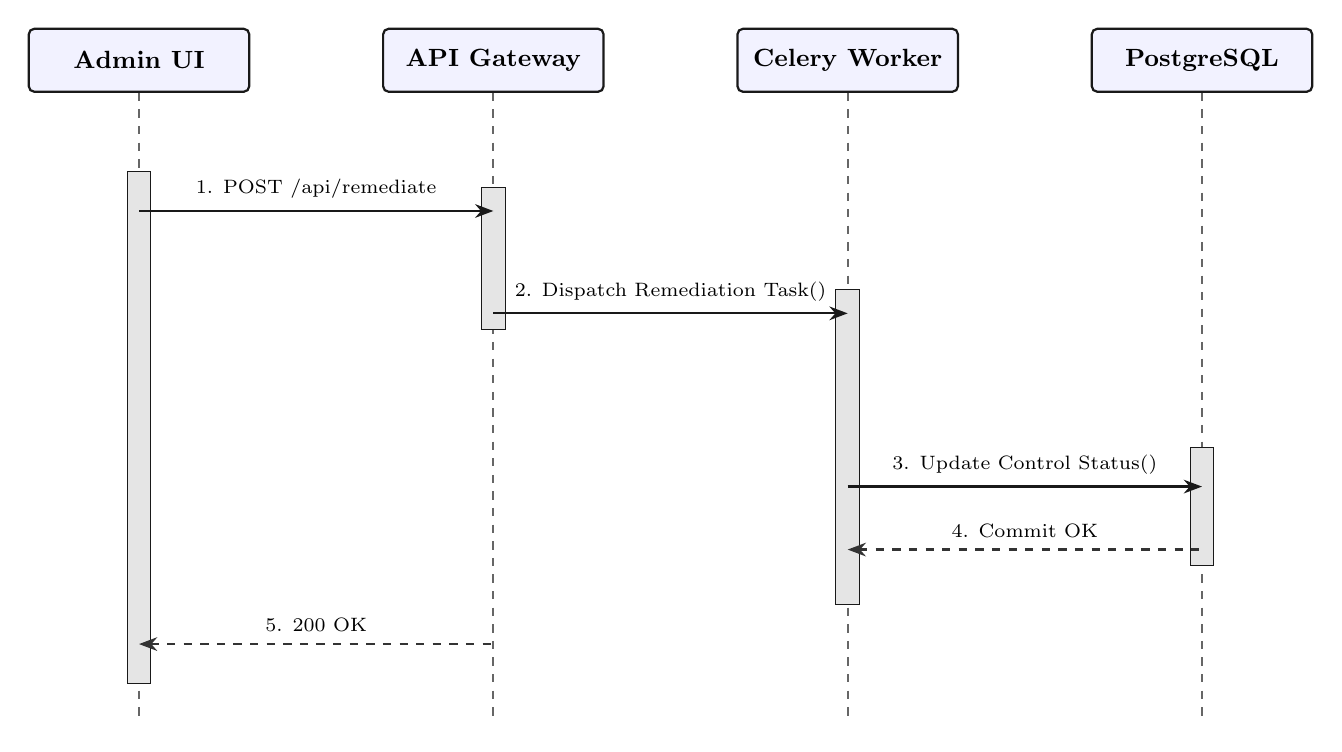
\begin{tikzpicture}[
        node distance=2cm,
        inst/.style={rectangle, draw=black!90, thick, fill=blue!5, minimum width=2.8cm, minimum height=0.8cm, font=\small\bfseries, rounded corners=2pt},
        act/.style={rectangle, draw=black!90, fill=gray!20, minimum width=0.3cm},
        msg/.style={-Stealth, thick, draw=black!90},
        reply/.style={Stealth-, thick, dashed, draw=black!80},
        label/.style={font=\scriptsize, inner sep=2pt}
    ]
        \node[inst] (client) at (0, 0) {Admin UI};
        \node[inst] (api) at (4.5, 0) {API Gateway};
        \node[inst] (celery) at (9, 0) {Celery Worker};
        \node[inst] (db) at (13.5, 0) {PostgreSQL};
        \draw[dashed, draw=black!60, thick] (client.south) -- ++(0, -8);
        \draw[dashed, draw=black!60, thick] (api.south) -- ++(0, -8);
        \draw[dashed, draw=black!60, thick] (celery.south) -- ++(0, -8);
        \draw[dashed, draw=black!60, thick] (db.south) -- ++(0, -8);
        \draw[act] ([xshift=-0.15cm, yshift=-1cm]client.south) rectangle ([xshift=0.15cm, yshift=-7.5cm]client.south);
        \draw[act] ([xshift=-0.15cm, yshift=-1.2cm]api.south) rectangle ([xshift=0.15cm, yshift=-3cm]api.south);
        \draw[act] ([xshift=-0.15cm, yshift=-2.5cm]celery.south) rectangle ([xshift=0.15cm, yshift=-6.5cm]celery.south);
        \draw[act] ([xshift=-0.15cm, yshift=-4.5cm]db.south) rectangle ([xshift=0.15cm, yshift=-6cm]db.south);
        \draw[msg] ([yshift=-1.5cm]client.south) -- ([yshift=-1.5cm]api.south) node[midway, above=2pt, label] {1. POST /api/remediate};
        \draw[msg] ([yshift=-2.8cm]api.south) -- ([yshift=-2.8cm]celery.south) node[midway, above=2pt, label] {2. Dispatch Remediation Task()};
        \draw[msg] ([yshift=-5cm]celery.south) -- ([yshift=-5cm]db.south) node[midway, above=2pt, label] {3. Update Control Status()};
        \draw[reply] ([yshift=-5.8cm]celery.south) -- ([yshift=-5.8cm]db.south) node[midway, above=2pt, label] {4. Commit OK};
        \draw[reply] ([yshift=-7cm]client.south) -- ([yshift=-7cm]api.south) node[midway, above=2pt, label] {5. 200 OK};
    \end{tikzpicture}
    }
    \caption{SD-05-1: Resolve Compliance Anomalies}
    \label{fig:sd_05_1}
\end{figure}

\subsubsection{SD-06: Export Audit Reports}
This sequence traces UC-06, the PDF audit report generation pipeline. The auditor requests a compliance report, the API queries historical data from PostgreSQL, renders the PDF binary, and streams it back to the client browser.

Figure \ref{fig:sd_06_1} documents the report generation and delivery path.

\begin{figure}[H]
    \centering
    \resizebox{0.9\textwidth}{!}{
    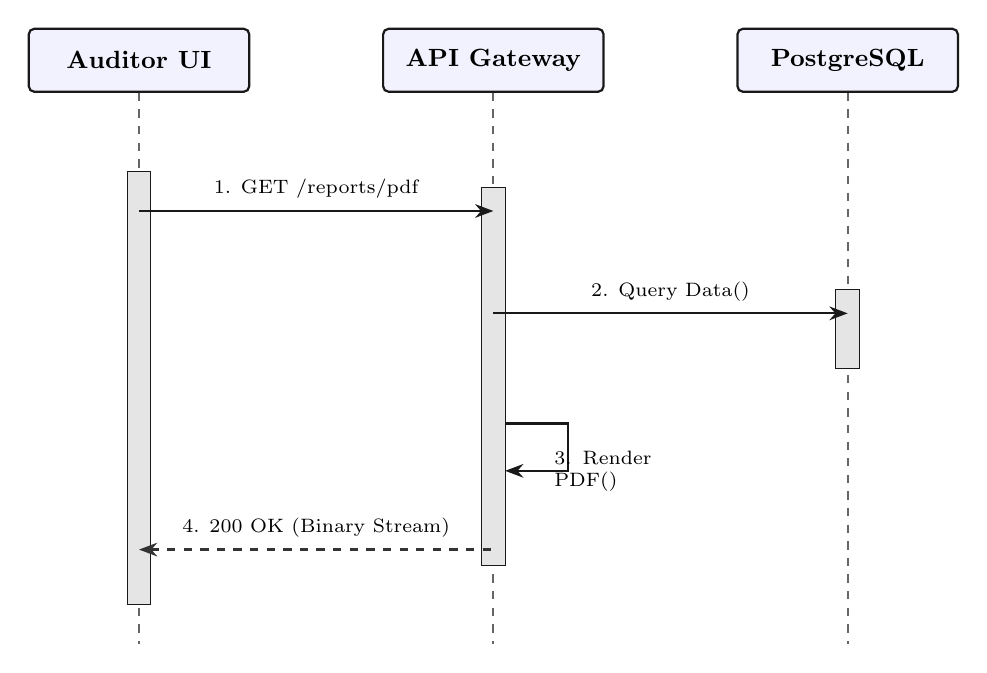
\begin{tikzpicture}[
        node distance=2cm,
        inst/.style={rectangle, draw=black!90, thick, fill=blue!5, minimum width=2.8cm, minimum height=0.8cm, font=\small\bfseries, rounded corners=2pt},
        act/.style={rectangle, draw=black!90, fill=gray!20, minimum width=0.3cm},
        msg/.style={-Stealth, thick, draw=black!90},
        reply/.style={Stealth-, thick, dashed, draw=black!80},
        label/.style={font=\scriptsize, inner sep=2pt}
    ]
        \node[inst] (client) at (0, 0) {Auditor UI};
        \node[inst] (api) at (4.5, 0) {API Gateway};
        \node[inst] (db) at (9, 0) {PostgreSQL};
        \draw[dashed, draw=black!60, thick] (client.south) -- ++(0, -7);
        \draw[dashed, draw=black!60, thick] (api.south) -- ++(0, -7);
        \draw[dashed, draw=black!60, thick] (db.south) -- ++(0, -7);
        \draw[act] ([xshift=-0.15cm, yshift=-1cm]client.south) rectangle ([xshift=0.15cm, yshift=-6.5cm]client.south);
        \draw[act] ([xshift=-0.15cm, yshift=-1.2cm]api.south) rectangle ([xshift=0.15cm, yshift=-6cm]api.south);
        \draw[act] ([xshift=-0.15cm, yshift=-2.5cm]db.south) rectangle ([xshift=0.15cm, yshift=-3.5cm]db.south);
        \draw[msg] ([yshift=-1.5cm]client.south) -- ([yshift=-1.5cm]api.south) node[midway, above=2pt, label] {1. GET /reports/pdf};
        \draw[msg] ([yshift=-2.8cm]api.south) -- ([yshift=-2.8cm]db.south) node[midway, above=2pt, label] {2. Query Data()};
        \draw[msg] ([yshift=-4.2cm]api.south) ++(0.15cm,0) -- ++(0.8,0) -- ++(0,-0.6) -- ++(-0.8,0) node[midway, right=4pt, label, text width=2cm] {3. Render PDF()};
        \draw[reply] ([yshift=-5.8cm]client.south) -- ([yshift=-5.8cm]api.south) node[midway, above=2pt, label] {4. 200 OK (Binary Stream)};
    \end{tikzpicture}
    }
    \caption{SD-06-1: Report Generation}
    \label{fig:sd_06_1}
\end{figure}


\section{Low Level Design}
The Low-Level Design (LLD) translates the high-level system architecture into fundamental software building blocks. This section maps the specific object-oriented structures, persistence models, and relational bindings that dictate the execution of the ISCMS platform's core business logic.

\subsection{UML Class Diagram}
Figure \ref{fig:class_diagram} shows the Django ORM classes and their relationships. Relational constraints link regulatory frameworks to specific endpoint telemetry logs.

\begin{figure}[H]
    \centering
    \resizebox{\textwidth}{!}{
    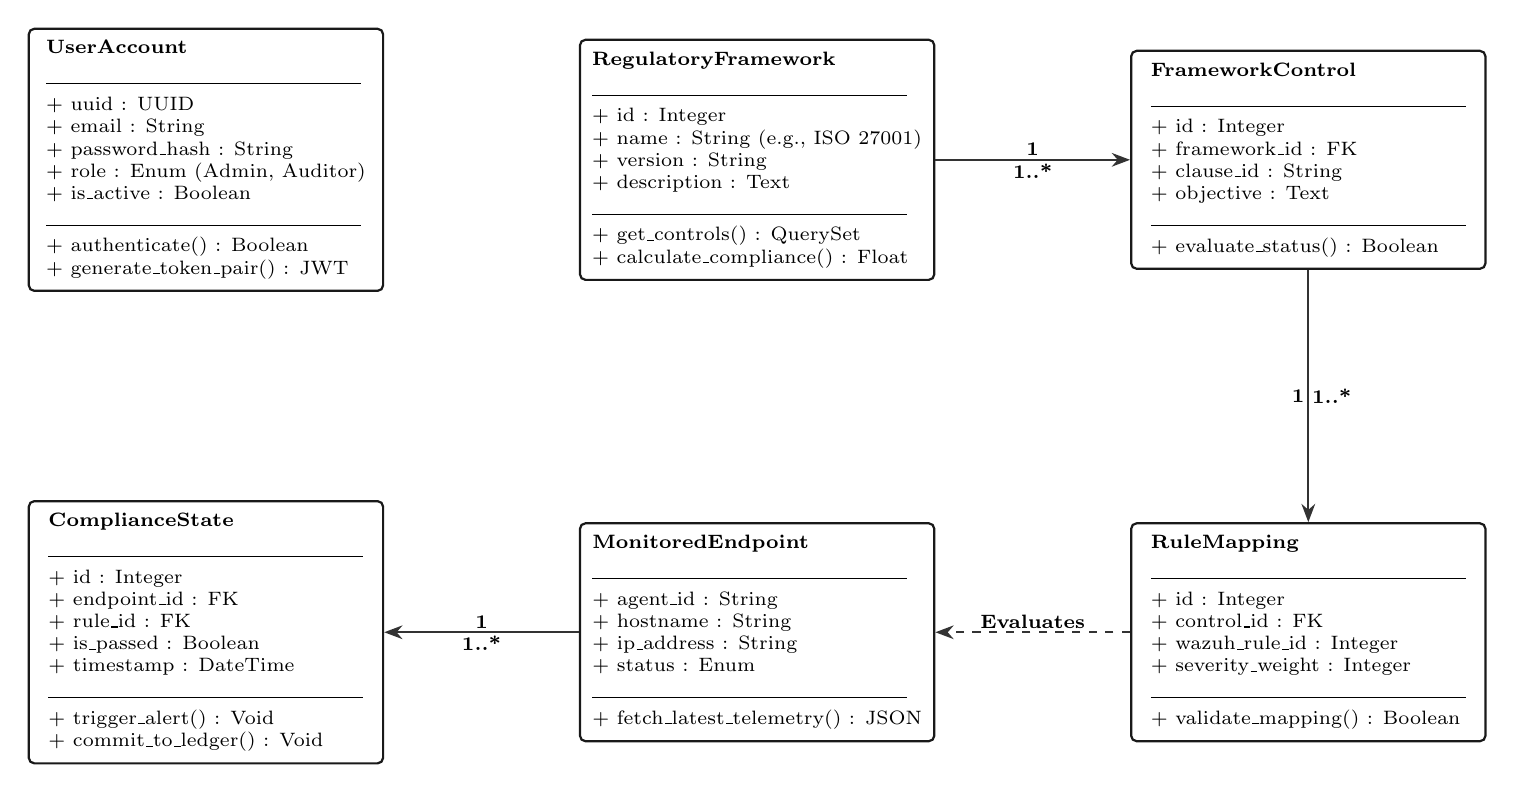
\begin{tikzpicture}[
        classnode/.style={rectangle, draw=black!90, thick, fill=white, align=left, minimum width=4.5cm, rounded corners=2pt, inner sep=1ex, font=\scriptsize},
        assoc/.style={-Stealth, thick, draw=black!80},
        rel/.style={font=\scriptsize\bfseries, fill=white, inner sep=1pt}
    ]
        % Classes
        \node[classnode] (user) at (0, 0) {
            \textbf{UserAccount}\\[1ex]
            \rule{4cm}{0.4pt}\\[0.5ex]
            + uuid : UUID\\
            + email : String\\
            + password\_hash : String\\
            + role : Enum (Admin, Auditor)\\
            + is\_active : Boolean\\[0.5ex]
            \rule{4cm}{0.4pt}\\[0.5ex]
            + authenticate() : Boolean\\
            + generate\_token\_pair() : JWT
        };
        \node[classnode] (framework) at (7, 0) {
            \textbf{RegulatoryFramework}\\[1ex]
            \rule{4cm}{0.4pt}\\[0.5ex]
            + id : Integer\\
            + name : String (e.g., ISO 27001)\\
            + version : String\\
            + description : Text\\[0.5ex]
            \rule{4cm}{0.4pt}\\[0.5ex]
            + get\_controls() : QuerySet\\
            + calculate\_compliance() : Float
        };
        \node[classnode] (control) at (14, 0) {
            \textbf{FrameworkControl}\\[1ex]
            \rule{4cm}{0.4pt}\\[0.5ex]
            + id : Integer\\
            + framework\_id : FK\\
            + clause\_id : String\\
            + objective : Text\\[0.5ex]
            \rule{4cm}{0.4pt}\\[0.5ex]
            + evaluate\_status() : Boolean
        };
        \node[classnode] (mapping) at (14, -6) {
            \textbf{RuleMapping}\\[1ex]
            \rule{4cm}{0.4pt}\\[0.5ex]
            + id : Integer\\
            + control\_id : FK\\
            + wazuh\_rule\_id : Integer\\
            + severity\_weight : Integer\\[0.5ex]
            \rule{4cm}{0.4pt}\\[0.5ex]
            + validate\_mapping() : Boolean
        };
        \node[classnode] (endpoint) at (7, -6) {
            \textbf{MonitoredEndpoint}\\[1ex]
            \rule{4cm}{0.4pt}\\[0.5ex]
            + agent\_id : String\\
            + hostname : String\\
            + ip\_address : String\\
            + status : Enum\\[0.5ex]
            \rule{4cm}{0.4pt}\\[0.5ex]
            + fetch\_latest\_telemetry() : JSON
        };
        \node[classnode] (state) at (0, -6) {
            \textbf{ComplianceState}\\[1ex]
            \rule{4cm}{0.4pt}\\[0.5ex]
            + id : Integer\\
            + endpoint\_id : FK\\
            + rule\_id : FK\\
            + is\_passed : Boolean\\
            + timestamp : DateTime\\[0.5ex]
            \rule{4cm}{0.4pt}\\[0.5ex]
            + trigger\_alert() : Void\\
            + commit\_to\_ledger() : Void
        };
        % Relationships
        \draw[assoc] (framework.east) -- (control.west) node[midway, above, rel] {1} node[midway, below, rel] {1..*};
        \draw[assoc] (control.south) -- (mapping.north) node[midway, left, rel] {1} node[midway, right, rel] {1..*};
        \draw[assoc] (endpoint.west) -- (state.east) node[midway, above, rel] {1} node[midway, below, rel] {1..*};
        \draw[assoc, dashed] (mapping.west) -- (endpoint.east) node[midway, above, rel] {Evaluates};
        
    \end{tikzpicture}
    }
    \caption{UML Class Diagram: Core Object-Relational Models}
    \label{fig:class_diagram}
\end{figure}

\section{Database Design}
I built the database on PostgreSQL. The tables are normalized to the Third Normal Form (3NF) to prevent update anomalies. When you're pulling in thousands of SIEM alerts an hour, you need strict ACID compliance so the data doesn't corrupt.

\subsection{Physical Data Model (Core ERD)}
Figure \ref{fig:core_erd} shows the actual physical schema. I mapped out the exact column types and foreign keys we used to build the PostgreSQL database.

\begin{figure}[H]
    \centering
    \resizebox{\textwidth}{!}{
    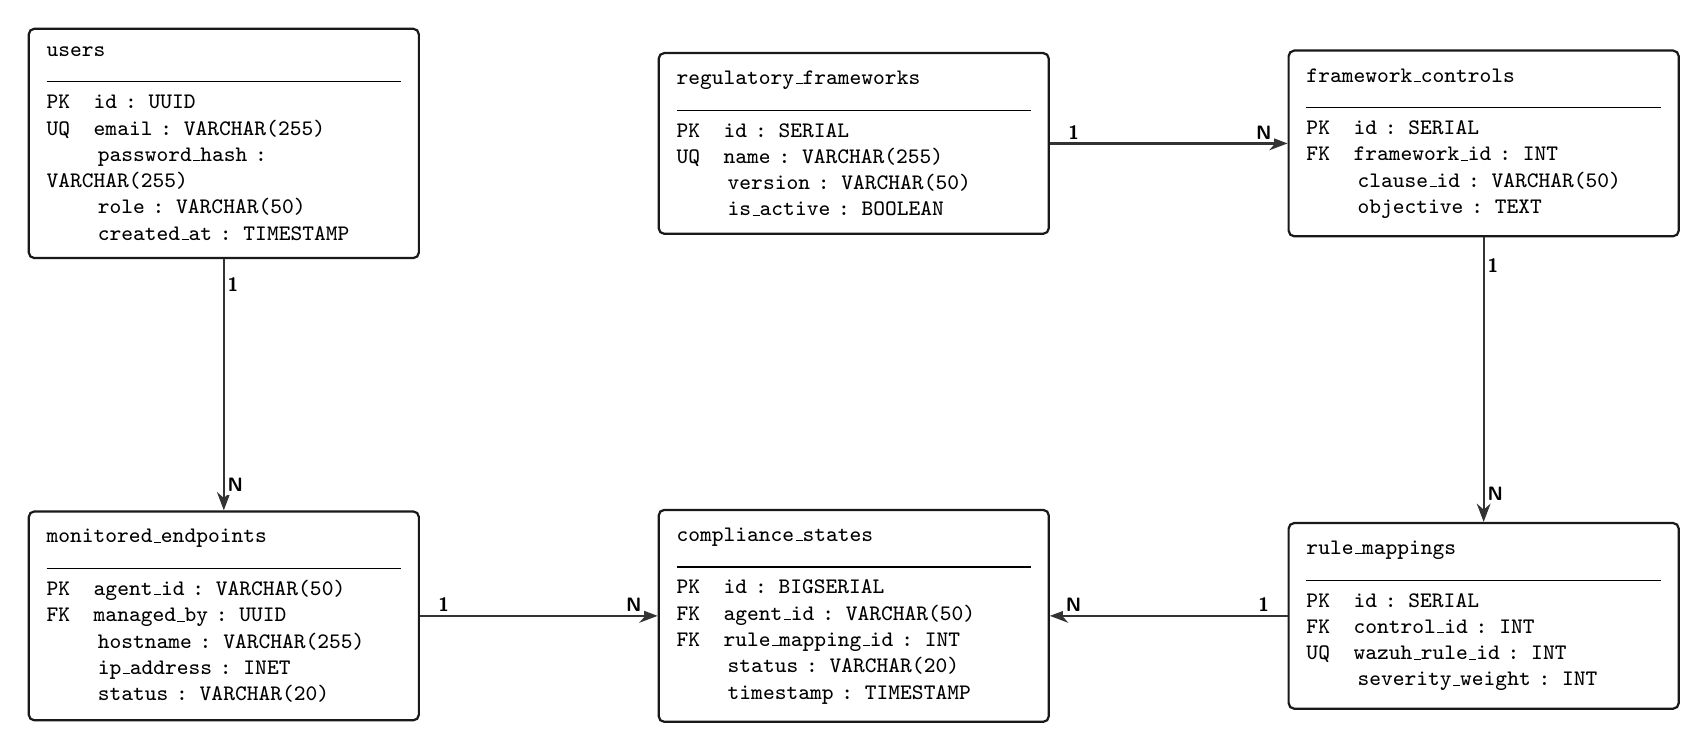
\begin{tikzpicture}[
        table/.style={rectangle, draw=black!90, thick, fill=white, align=left, font=\footnotesize\ttfamily, inner sep=1.5ex, rounded corners=2pt},
        rel/.style={-Stealth, thick, draw=black!80},
        card/.style={font=\scriptsize\bfseries\sffamily, fill=white, inner sep=1pt}
    ]

        % ----------------------------------------------------
        % TABLE PLACEMENT (Strict Grid Layout)
        % ----------------------------------------------------
        \node[table, text width=4.5cm] (users) at (0, 6) {
            \textbf{users} \\
            \rule{4.5cm}{0.4pt} \\
            PK \hspace{1mm} id : UUID \\
            UQ \hspace{1mm} email : VARCHAR(255) \\
            \hspace{5.5mm} password\_hash : VARCHAR(255) \\
            \hspace{5.5mm} role : VARCHAR(50) \\
            \hspace{5.5mm} created\_at : TIMESTAMP
        };

        \node[table, text width=4.5cm] (frameworks) at (8, 6) {
            \textbf{regulatory\_frameworks} \\
            \rule{4.5cm}{0.4pt} \\
            PK \hspace{1mm} id : SERIAL \\
            UQ \hspace{1mm} name : VARCHAR(255) \\
            \hspace{5.5mm} version : VARCHAR(50) \\
            \hspace{5.5mm} is\_active : BOOLEAN
        };

        \node[table, text width=4.5cm] (controls) at (16, 6) {
            \textbf{framework\_controls} \\
            \rule{4.5cm}{0.4pt} \\
            PK \hspace{1mm} id : SERIAL \\
            FK \hspace{1mm} framework\_id : INT \\
            \hspace{5.5mm} clause\_id : VARCHAR(50) \\
            \hspace{5.5mm} objective : TEXT
        };

        \node[table, text width=4.5cm] (endpoints) at (0, 0) {
            \textbf{monitored\_endpoints} \\
            \rule{4.5cm}{0.4pt} \\
            PK \hspace{1mm} agent\_id : VARCHAR(50) \\
            FK \hspace{1mm} managed\_by : UUID \\
            \hspace{5.5mm} hostname : VARCHAR(255) \\
            \hspace{5.5mm} ip\_address : INET \\
            \hspace{5.5mm} status : VARCHAR(20)
        };

        \node[table, text width=4.5cm] (states) at (8, 0) {
            \textbf{compliance\_states} \\
            \rule{4.5cm}{0.4pt} \\
            PK \hspace{1mm} id : BIGSERIAL \\
            FK \hspace{1mm} agent\_id : VARCHAR(50) \\
            FK \hspace{1mm} rule\_mapping\_id : INT \\
            \hspace{5.5mm} status : VARCHAR(20) \\
            \hspace{5.5mm} timestamp : TIMESTAMP
        };

        \node[table, text width=4.5cm] (mappings) at (16, 0) {
            \textbf{rule\_mappings} \\
            \rule{4.5cm}{0.4pt} \\
            PK \hspace{1mm} id : SERIAL \\
            FK \hspace{1mm} control\_id : INT \\
            UQ \hspace{1mm} wazuh\_rule\_id : INT \\
            \hspace{5.5mm} severity\_weight : INT
        };

        % ----------------------------------------------------
        % RELATIONSHIPS (Crow's Foot via 1-to-N lines)
        % ----------------------------------------------------
        \draw[rel] (users.south) -- (endpoints.north) node[pos=0.1, right, card] {1} node[pos=0.9, right, card] {N};
        \draw[rel] (frameworks.east) -- (controls.west) node[pos=0.1, above, card] {1} node[pos=0.9, above, card] {N};
        \draw[rel] (controls.south) -- (mappings.north) node[pos=0.1, right, card] {1} node[pos=0.9, right, card] {N};
        \draw[rel] (endpoints.east) -- (states.west) node[pos=0.1, above, card] {1} node[pos=0.9, above, card] {N};
        \draw[rel] (mappings.west) -- (states.east) node[pos=0.1, above, card] {1} node[pos=0.9, above, card] {N};

    \end{tikzpicture}
    }
    \caption{Physical Database Schema: Core Relational Data Model with Exact Data Types}
    \label{fig:core_erd}
\end{figure}

\subsection{Extended Entity Relationship Diagram (EERD)}
Figure \ref{fig:eerd} is an Extended ERD (EERD) that visualizes the logical rules we put in place.

Notice the disjoint (\textbf{d}) specialization: a generic User Account splits strictly into either a System Admin or a Security Auditor. That handles our RBAC at the database level. I also modeled the Compliance State as a weak entity, because an alert record is useless without its parent Monitored Endpoint.

\begin{figure}[H]
    \centering
    \resizebox{0.9\textwidth}{!}{
    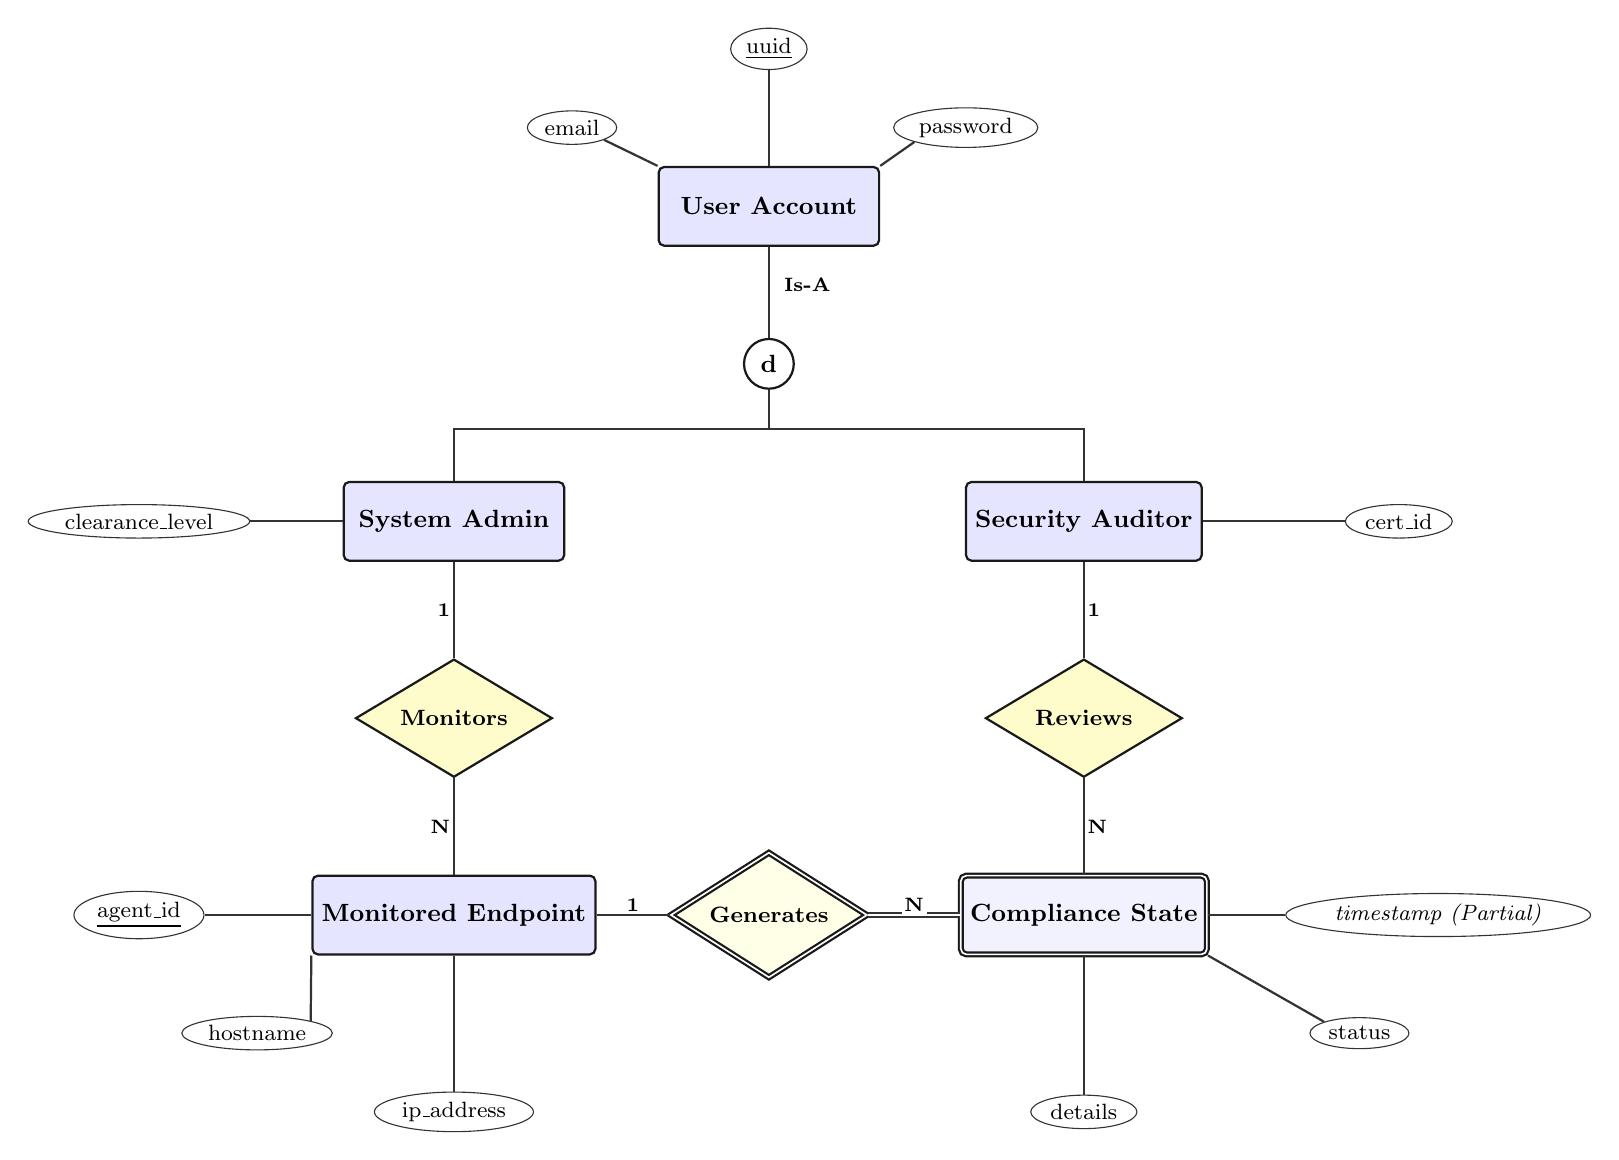
\begin{tikzpicture}[
        entity/.style={rectangle, draw=black!90, thick, fill=blue!10, minimum width=2.8cm, minimum height=1cm, align=center, font=\small\bfseries, rounded corners=2pt},
        weakent/.style={rectangle, double, draw=black!90, thick, fill=blue!5, minimum width=2.8cm, minimum height=1cm, align=center, font=\small\bfseries, rounded corners=2pt},
        rel/.style={diamond, draw=black!90, thick, fill=yellow!20, minimum width=2.5cm, minimum height=1.5cm, align=center, font=\footnotesize\bfseries, aspect=1.5},
        weakrel/.style={diamond, double, draw=black!90, thick, fill=yellow!10, minimum width=2.5cm, minimum height=1.5cm, align=center, font=\footnotesize\bfseries, aspect=1.5},
        disjoint/.style={circle, draw=black!90, thick, fill=white, minimum size=0.6cm, font=\small\bfseries},
        line/.style={thick, draw=black!80},
        attr/.style={ellipse, draw=black!80, fill=white, font=\footnotesize, inner sep=1.5pt},
        card/.style={font=\scriptsize\bfseries, fill=white, inner sep=1pt}
    ]

        % ----------------------------------------------------
        % CORE ENTITIES (Center Y-Axis Stack)
        % ----------------------------------------------------
        \node[entity] (user) at (0, 5) {User Account};
        \node[disjoint] (d) at (0, 3) {d};
        \node[font=\scriptsize\bfseries, right=2pt] at (0, 4) {Is-A};
        
        \node[entity] (admin) at (-4, 1) {System Admin};
        \node[entity] (auditor) at (4, 1) {Security Auditor};

        \node[rel] (monitors) at (-4, -1.5) {Monitors};
        \node[rel] (reviews) at (4, -1.5) {Reviews};

        \node[entity] (endpoint) at (-4, -4) {Monitored Endpoint};
        \node[weakrel] (generates) at (0, -4) {Generates};
        \node[weakent] (state) at (4, -4) {Compliance State};

        % ----------------------------------------------------
        % ATTRIBUTES (Shooting Outwards to Prevent Overlap)
        % ----------------------------------------------------
        % User Attributes (Top)
        \node[attr] (uuid) at (0, 7) {\underline{uuid}};
        \node[attr] (email) at (-2.5, 6) {email};
        \node[attr] (pass) at (2.5, 6) {password};
        \draw[line] (user.north) -- (uuid.south);
        \draw[line] (user.north west) -- (email.south east);
        \draw[line] (user.north east) -- (pass.south west);

        % Subclass Attributes (Far Left / Far Right)
        \node[attr] (clearance) at (-8.0, 1) {clearance\_level};
        \draw[line] (admin.west) -- (clearance.east);

        \node[attr] (cert) at (8.0, 1) {cert\_id};
        \draw[line] (auditor.east) -- (cert.west);

        % Endpoint Attributes (Bottom Left)
        \node[attr] (agent) at (-8.0, -4) {\underline{agent\_id}};
        \node[attr] (hostname) at (-6.5, -5.5) {hostname};
        \node[attr] (ip) at (-4, -6.5) {ip\_address};
        \draw[line] (endpoint.west) -- (agent.east);
        \draw[line] (endpoint.south west) -- (hostname.north east);
        \draw[line] (endpoint.south) -- (ip.north);

        % State Attributes (Bottom Right)
        \node[attr] (timestamp) at (8.5, -4) {\textit{timestamp (Partial)}};
        \node[attr] (status) at (7.5, -5.5) {status};
        \node[attr] (details) at (4, -6.5) {details};
        \draw[line] (state.east) -- (timestamp.west);
        \draw[line] (state.south east) -- (status.north west);
        \draw[line] (state.south) -- (details.north);

        % ----------------------------------------------------
        % STRUCTURAL CONNECTIONS
        % ----------------------------------------------------
        % Inheritance
        \draw[line] (user.south) -- (d.north);
        \draw[line] (d.south) -- ++(0,-0.5) -| (admin.north);
        \draw[line] (d.south) -- ++(0,-0.5) -| (auditor.north);

        % Admin to Endpoint
        \draw[line] (admin.south) -- (monitors.north) node[midway, left, card] {1};
        \draw[line] (monitors.south) -- (endpoint.north) node[midway, left, card] {N};

        % Auditor to State
        \draw[line] (auditor.south) -- (reviews.north) node[midway, right, card] {1};
        \draw[line] (reviews.south) -- (state.north) node[midway, right, card] {N};

        % Weak Entity Dependency
        \draw[line] (endpoint.east) -- (generates.west) node[midway, above, card] {1};
        \draw[line, double] (generates.east) -- (state.west) node[midway, above, card] {N};

    \end{tikzpicture}
    }
    \caption{Extended Entity Relationship Diagram (EERD) with Constraints and Attributes}
    \label{fig:eerd}
\end{figure}


\section{Graphical User Interface (GUI) Design}
The frontend is a React Single Page Application (SPA) designed to present compliance telemetry without visual clutter. The screenshots below demonstrate the default dark mode, though the application supports dynamic theme switching.

\subsection{Authentication and Identity Management}
The authentication portal validates user credentials and issues a JSON Web Token (JWT). The application then initializes the dashboard corresponding to the user's RBAC role.

\begin{figure}[H]
    \centering
    \includegraphics[width=1.0\textwidth]{"images/login.png"}
    \caption{GUI Design: Secure User Authentication Portal.}
    \label{fig:gui_login}
\end{figure}

\begin{figure}[H]
    \centering
    \includegraphics[width=1.0\textwidth]{"images/2fa.png"}
    \caption{GUI Design: Time-based One-Time Password (TOTP) Verification.}
    \label{fig:gui_2fa}
\end{figure}

\subsection{Superadmin Configuration Portal}
Superadmins have full administrative privileges, including configuration of the Wazuh pipeline, regulatory mapping rules, and user account provisioning. The interface supports dynamic theming for varied lighting conditions.

\begin{figure}[H]
    \centering
    \includegraphics[width=1.0\textwidth]{"images/superadmin dashboard dark.png"}
    \caption{GUI Design: Superadmin Global Compliance Dashboard (Dark Mode).}
    \label{fig:gui_superadmin_dark}
\end{figure}

\begin{figure}[H]
    \centering
    \includegraphics[width=1.0\textwidth]{"images/superadmin dashboard1.png"}
    \caption{GUI Design: Superadmin Global Compliance Dashboard (Light Mode).}
    \label{fig:gui_superadmin_light}
\end{figure}

\begin{figure}[H]
    \centering
    \includegraphics[width=1.0\textwidth]{"images/manage admins1.png"}
    \caption{GUI Design: RBAC User and System Administrator Management Interface.}
    \label{fig:gui_manage_admins}
\end{figure}

\subsection{Auditor Workspace (RBAC Enforcement)}
The application modifies the render tree based on the authenticated role. Auditors are restricted to a read-only interface to prevent unauthorized modifications to audit evidence or framework rules. Configuration and management modules are omitted from this view.

\begin{figure}[H]
    \centering
    \includegraphics[width=1.0\textwidth]{"images/auditor dashboard.png"}
    \caption{GUI Design: Security Auditor Read-Only Compliance View.}
    \label{fig:gui_auditor_dashboard}
\end{figure}

\subsection{Automated Audit Artifacts and Notifications}
The system provides PDF audit reports for external reviewers and SMTP alerts for administrators. The backend service aggregates PostgreSQL data to generate these artifacts and sends notifications when compliance thresholds are breached.

\begin{figure}[H]
    \centering
    \includegraphics[width=1.0\textwidth]{"images/compliance report pdf.png"}
    \caption{System Output: Automated PDF Audit Dossier Generation.}
    \label{fig:gui_pdf_report}
\end{figure}

\begin{figure}[H]
    \centering
    \includegraphics[width=1.0\textwidth]{"images/email.png"}
    \caption{System Output: SMTP Alert for Rule Violation.}
    \label{fig:gui_email_alert}
\end{figure}


\section{External Interfaces}
The ISCMS doesn't run in a vacuum. It talks to several external services. This section lists out the protocols and authentication methods I used to keep those connections secure.

\subsection{Wazuh SIEM REST API}
The whole system relies on raw logs coming from the Wazuh Manager. My Celery workers hit the Wazuh REST API over HTTPS. I secured this with Bearer tokens generated by the Wazuh server. We pull down the JSON payloads and validate them against the Django ORM before saving them.

\subsection{SMTP Notification Gateway}
For real-time alerts, the backend constructs HTML emails and fires them off through an external SMTP server over port 587 using STARTTLS. I threw this logic into the async message broker so it wouldn't block the API Gateway.

\subsection{Outbound Webhook Integration}
I also added outbound webhooks so the system can talk to tools like Slack or Microsoft Teams. Whenever a compliance rule breaks, it shoots out an HTTP POST request with the JSON event data. To prevent spoofing, I added an HMAC-SHA256 signature to the headers.

\subsection{Interface Specification Matrix}
Table \ref{tab:external_interfaces} summarizes the technical parameters and boundary constraints of the platform's external interfaces.

\begin{table}[H]
    \centering
    \caption{External Interface Technical Specifications}
    \label{tab:external_interfaces}
    \renewcommand{\arraystretch}{1.4}
    \resizebox{0.95\textwidth}{!}{
    \begin{tabular}{|l|l|l|l|l|}
        \hline
        \rowcolor{blue!10} 
        \textbf{Interface Target} & \textbf{Network Protocol} & \textbf{Data Format} & \textbf{Authentication Mechanism} & \textbf{Directionality} \\ \hline
        Wazuh Manager API & HTTPS (TCP 443) & JSON & Bearer Token / API Key & Bidirectional (Polling) \\ \hline
        SMTP Relay Server & SMTP (TCP 587) & MIME / HTML & SMTP AUTH (TLS) & Outbound Only \\ \hline
        Enterprise Webhooks & HTTPS (TCP 443) & JSON & HMAC-SHA256 Signatures & Outbound Only \\ \hline
        Client Web Browser & HTTPS (TCP 443) & HTML / JSON & JWT (Stateless) & Bidirectional \\ \hline
    \end{tabular}
    }
\end{table}

% \chapter{Implementation}

The design phase established what the ICMS platform needed to do and how its components should relate to each other. This chapter documents the process of actually building it. Translating the architectural diagrams from Chapter~4 into working code involved some practical realities that shaped our final decisions: hardware constraints, Docker networking quirks, and the challenge of wiring together a Python backend, a JavaScript frontend, and an external SIEM running on a separate physical machine. The following sections walk through each layer of the implementation, grounded in the actual codebase.

All development was done on consumer-grade hardware running Windows and Ubuntu in a distributed home-lab setup. The Wazuh SIEM manager ran on a dedicated laptop at a fixed IP address (\url{192.168.100.100}), and the full backend, frontend, and database stack was containerized on a second machine using Docker Compose. Every service configuration, environment variable, and migration step described here corresponds directly to the files in the project repository.

\section{System Architecture}

As established in the design phase (as shown below in Figure \ref{fig:tier_architecture_impl}), the ICMS platform follows an N-tier client-server architecture.

\begin{figure}[H]
    \centering
    \resizebox{0.85\textwidth}{!}{
    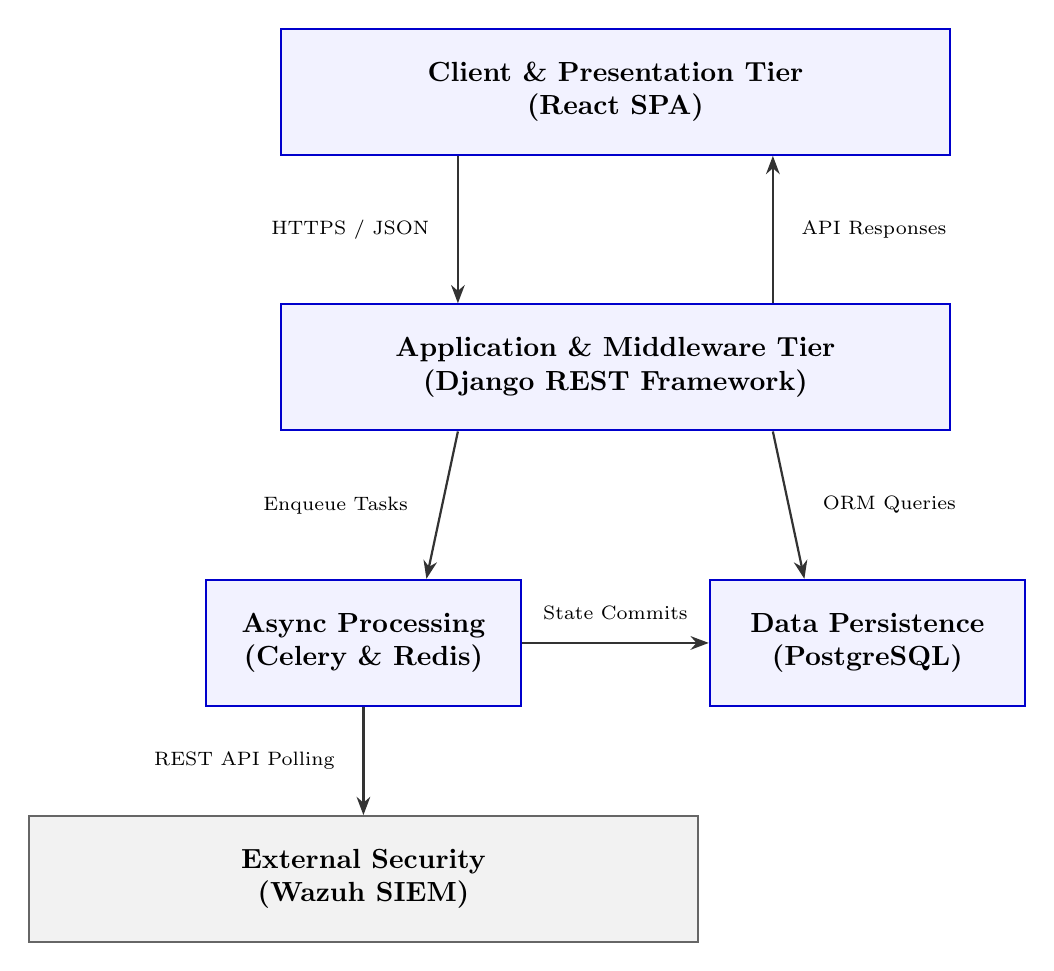
\begin{tikzpicture}[
        tier/.style={rectangle, draw=blue!80!black, thick, fill=blue!5, minimum width=8.5cm, minimum height=1.6cm, align=center, font=\bfseries},
        arrow/.style={-Stealth, thick, draw=black!80},
        label/.style={font=\scriptsize, inner sep=2pt}
    ]
        % Tiers with increased separation to resolve congestion
        \node[tier] (client) at (0, 8.5) {Client \& Presentation Tier\\(React SPA)};
        \node[tier] (app) at (0, 5.0) {Application \& Middleware Tier\\(Django REST Framework)};
        
        \node[tier, minimum width=4cm] (async) at (-3.2, 1.5) {Async Processing\\(Celery \& Redis)};
        \node[tier, minimum width=4cm] (data) at (3.2, 1.5) {Data Persistence\\(PostgreSQL)};
        
        \node[tier, fill=gray!10, draw=gray!80!black] (wazuh) at (-3.2, -1.5) {External Security\\(Wazuh SIEM)};

        % Client <-> App Connections
        \draw[arrow] ([xshift=-2cm]client.south) -- ([xshift=-2cm]app.north) 
            node[midway, left=8pt, label] {HTTPS / JSON};
        \draw[arrow] ([xshift=2cm]app.north) -- ([xshift=2cm]client.south) 
            node[midway, right=8pt, label] {API Responses};

        % App -> Async / Data Connections (Widened entry points)
        \draw[arrow] ([xshift=-2cm]app.south) -- ([xshift=0.8cm]async.north) 
            node[midway, left=10pt, label] {Enqueue Tasks};
        \draw[arrow] ([xshift=2cm]app.south) -- ([xshift=-0.8cm]data.north) 
            node[midway, right=10pt, label] {ORM Queries};

        % Async -> Wazuh (Increased vertical gap)
        \draw[arrow] (async.south) -- (wazuh.north) 
            node[midway, left=8pt, label] {REST API Polling};
        
        % Async -> Data (Increased horizontal gap)
        \draw[arrow] (async.east) -- (data.west) 
            node[midway, above=6pt, label] {State Commits};
    \end{tikzpicture}
    }
    \caption{Implemented N-Tier System Architecture}
    \label{fig:tier_architecture_impl}
\end{figure}

In practice, this mapped onto two concrete code repositories: a \url{backend/} directory containing the Django application and all its sub-apps, and a \url{frontend/} directory containing the React SPA. Both are wired together through a \url{docker-compose.yml} file at the project root that defines seven services and a shared bridge network.

The full service topology (as shown below in Figure \ref{fig:deployment_diagram_impl}) illustrates the container environment and network isolation.

\begin{figure}[H]
    \centering
    \resizebox{0.95\textwidth}{!}{
    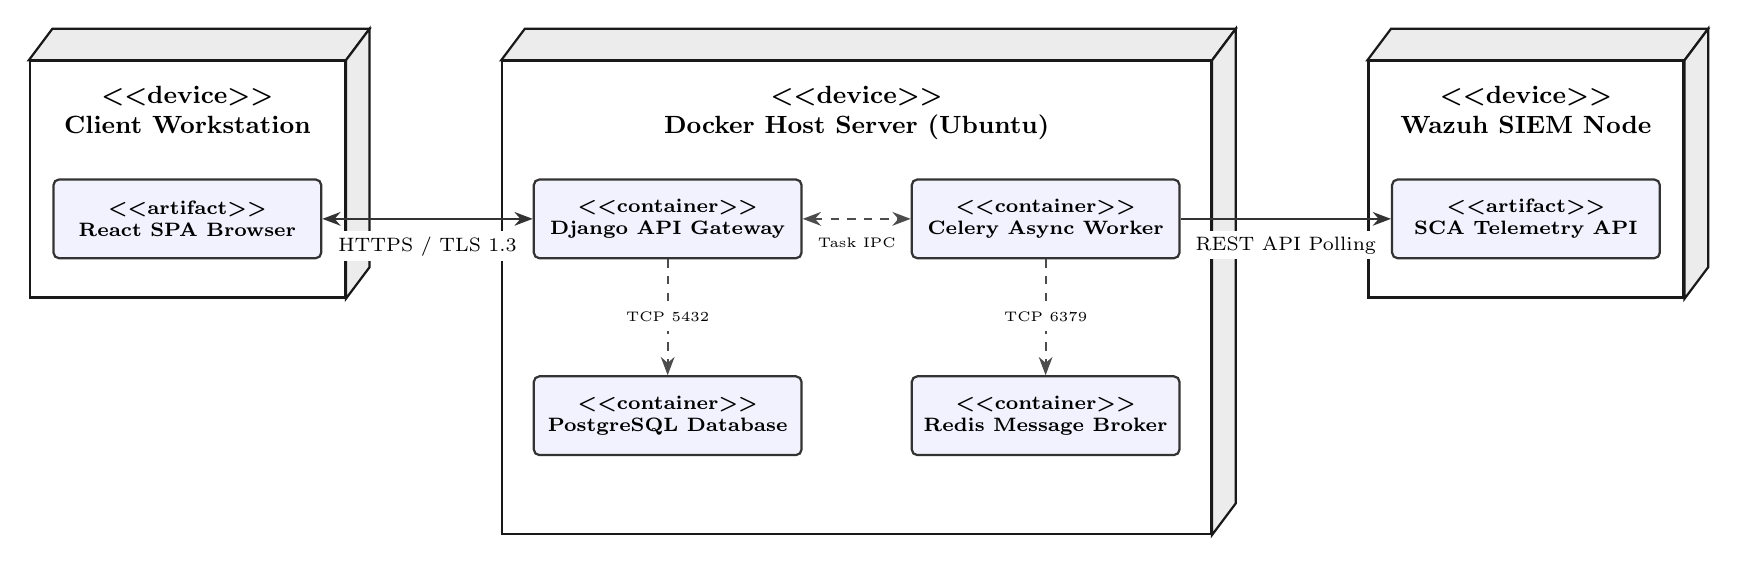
\begin{tikzpicture}[
        device/.style={
            rectangle, draw=black!90, thick, fill=white,
            minimum width=4cm, minimum height=2.5cm,
            append after command={
                \pgfextra{
                    \filldraw[black!90, thick, fill=gray!15] (\tikzlastnode.north west) -- ++(0.3, 0.4) -- ($(\tikzlastnode.north east)+(0.3,0.4)$) -- (\tikzlastnode.north east) -- cycle;
                    \filldraw[black!90, thick, fill=gray!15] (\tikzlastnode.north east) -- ($(\tikzlastnode.north east)+(0.3,0.4)$) -- ($(\tikzlastnode.south east)+(0.3,0.4)$) -- (\tikzlastnode.south east) -- cycle;
                }
            }
        },
        artifact/.style={
            rectangle, draw=black!80, thick, fill=blue!5,
            minimum width=3.4cm, minimum height=1cm,
            align=center, font=\scriptsize\bfseries, rounded corners=2pt
        },
        conn/.style={
            thick, draw=black!80, Stealth-Stealth
        },
        label/.style={
            font=\scriptsize, fill=white, inner sep=2pt
        }
    ]
        % ----------------------------------------------------
        % CENTER: Docker Host Server
        % ----------------------------------------------------
        \node[device, minimum width=9cm, minimum height=6cm] (server) at (0, 0) {};
        \node[anchor=north, font=\small\bfseries, yshift=-2mm, align=center] at (server.north) {\textless\textless device\textgreater\textgreater\\Docker Host Server (Ubuntu)};
        
        \node[artifact] (django) at (-2.4, 1) {\textless\textless container\textgreater\textgreater\\Django API Gateway};
        \node[artifact] (celery) at (2.4, 1) {\textless\textless container\textgreater\textgreater\\Celery Async Worker};
        \node[artifact] (postgres) at (-2.4, -1.5) {\textless\textless container\textgreater\textgreater\\PostgreSQL Database};
        \node[artifact] (redis) at (2.4, -1.5) {\textless\textless container\textgreater\textgreater\\Redis Message Broker};

        % Internal Bridge Network Connections
        \draw[dashed, -Stealth, thick, draw=black!70] (django.south) -- (postgres.north) node[midway, fill=white, font=\tiny] {TCP 5432};
        \draw[dashed, -Stealth, thick, draw=black!70] (celery.south) -- (redis.north) node[midway, fill=white, font=\tiny] {TCP 6379};
        \draw[dashed, Stealth-Stealth, thick, draw=black!70] (django.east) -- (celery.west) node[midway, below=3pt, fill=white, font=\tiny] {Task IPC};

        % ----------------------------------------------------
        % LEFT: Client Workstation
        % ----------------------------------------------------
        \node[device, minimum width=4cm, minimum height=3cm] (client) at (-8.5, 1.5) {};
        \node[anchor=north, font=\small\bfseries, yshift=-2mm, align=center] at (client.north) {\textless\textless device\textgreater\textgreater\\Client Workstation};
        \node[artifact] (react) at (-8.5, 1) {\textless\textless artifact\textgreater\textgreater\\React SPA Browser};

        % ----------------------------------------------------
        % RIGHT: Wazuh SIEM Node
        % ----------------------------------------------------
        \node[device, minimum width=4cm, minimum height=3cm] (wazuh) at (8.5, 1.5) {};
        \node[anchor=north, font=\small\bfseries, yshift=-2mm, align=center] at (wazuh.north) {\textless\textless device\textgreater\textgreater\\Wazuh SIEM Node};
        \node[artifact] (sca) at (8.5, 1) {\textless\textless artifact\textgreater\textgreater\\SCA Telemetry API};

        % ----------------------------------------------------
        % EXTERNAL NETWORK CONNECTIONS (Perfectly Horizontal at Y=1)
        % ----------------------------------------------------
        \draw[conn] (react.east) -- (django.west) node[midway, below=4pt, label] {HTTPS / TLS 1.3};
        \draw[conn, -Stealth] (celery.east) -- (sca.west) node[midway, below=4pt, label] {REST API Polling};

    \end{tikzpicture}
    }
    \caption{Implemented Service Topology and Container Networking}
    \label{fig:deployment_diagram_impl}
\end{figure}

When the stack boots, Docker brings up the database and Redis first, waits for their health checks to pass, and only then starts the Django backend. This startup ordering was not optional; without it, the backend would crash on boot trying to run migrations against a database that was not yet accepting connections. The Celery worker and Celery Beat scheduler also depend on the backend image and start only after Redis is confirmed healthy.

\subsection{Presentation Layer Implementation (Frontend)}

The frontend is a React 19 Single Page Application built with Vite 8 as the build and development server. Vite was chosen over the older Create React App toolchain because it uses native ES modules during development, which cuts cold-start time from several seconds down to under 200ms. Routing is handled by React Router v7, which uses a declarative \texttt{<Route>} structure to enforce authentication boundaries at the component level.

Every HTTP request to the Django backend goes through an Axios instance configured with request and response interceptors. The request interceptor reads the JWT access token from \texttt{localStorage} and appends it as a \texttt{Bearer} header automatically. The response interceptor watches for \texttt{401 Unauthorized} responses; when one arrives, it triggers a token refresh and, if the refresh also fails, clears the session and redirects to the login page. This means we never had to write token-refresh logic in individual components.

The UI itself is styled with Tailwind CSS v4 using a custom \texttt{@theme} token set for brand colours, spacing, and typography. Data visualisation is handled by Recharts, which renders the compliance score gauge and per-framework bar charts on the main dashboard. Icon assets come from Lucide React. The routing table enforces RBAC at the frontend level too: the \texttt{/manage-admins} route requires the \texttt{required\allowbreak Role=``super\_admin''} prop on its \texttt{ProtectedRoute} wrapper, so Django's RBAC check at the API layer has a corresponding gate on the UI side.

\subsection{Middleware and API Gateway (Backend)}

The backend is a Django 5.1 project with a single installed application, \texttt{compliance}, that contains every model, view, serializer, and management command the platform needs. The project configuration lives in \texttt{core/settings.py}, and all secrets are loaded at startup via \texttt{python-decouple} from a \texttt{.env} file, so no credentials are ever hardcoded in source control.

Authentication is handled by \url{django-restframework-simplejwt}. Access tokens are valid for 24 hours; refresh tokens last seven days with rotation enabled, so each refresh call issues a new refresh token and invalidates the old one. The \texttt{Custom\allowbreak Token\allowbreak Obtain\allowbreak Pair\allowbreak View} overrides the standard login endpoint to add a two-factor authentication gate: if the user has TOTP enabled via \texttt{pyotp}, the view returns an intermediate \texttt{requires\_\allowbreak 2fa} flag instead of issuing tokens, forcing the client to complete a second verification round-trip before credentials are granted.

The \texttt{compliance} app's \url{views.py} contains both DRF ViewSets (for the standard CRUD resources like frameworks, controls, and policies) and custom \texttt{APIView} subclasses for complex operations such as dashboard aggregation and PDF report generation. The \texttt{Dashboard\allowbreak Summary\allowbreak View} is the most query-intensive endpoint in the system. It uses a single annotated queryset with \texttt{DISTINCT ON agent\_id} to find the latest scan per agent, then computes per-framework pass/fail counts using Django ORM \texttt{Count()} with \texttt{Q()} filter objects. This collapses what would otherwise be a na\"{i}ve N+1 loop across twenty-plus framework controls into a single SQL statement.

\subsection{Asynchronous Processing Engine}

Any time a compliance scan runs, it involves several seconds of HTTP polling against the external Wazuh REST API. Running that on the main Django request thread would block the server until the scan finished, effectively taking the dashboard offline for everyone else. The solution is to dispatch the work to a Celery worker process running in a separate container.

The Celery application is initialised in \url{core/celery.py}. It reads its configuration from Django settings using the \texttt{CELERY\_} namespace and calls \texttt{autodiscover\_tasks()} so it automatically picks up any \url{tasks.py} file across registered apps. The only task in the system is \texttt{run\_scheduled\_\allowbreak wazuh\_sync} in \url{compliance/tasks.py}, decorated with \texttt{@shared\_task(bind=True, max\_retries=3)}. The \texttt{bind=True} argument gives the task access to \texttt{self}, which it uses to call \texttt{self.retry(exc=exc, countdown=60)} when a Wazuh API call fails. This means a temporary network hiccup triggers an automatic 60-second backoff and retry rather than a permanent failure.

Redis runs as a separate container on port 6379 and acts as both the message broker and the result backend. The Celery Beat scheduler, also running as its own container, uses the \texttt{Database\allowbreak Scheduler} from \url{django-celery-beat}. This means scan frequency (daily, weekly, or monthly) is stored in the PostgreSQL database and can be changed at runtime through the Settings page in the UI, without restarting any containers. When a manual scan is triggered from the frontend, the \url{/api/run-scan/} endpoint receives a \texttt{POST} request, calls \texttt{run\_scheduled\_\allowbreak wazuh\_sync.delay()}, and immediately returns a \texttt{202 Accepted} response. The scan then runs in the worker container with no impact on the API's availability.

\subsection{Data Persistence Layer}

PostgreSQL 18 is the primary database, running in its own container and accessible to the Django backend and Celery worker over the Docker bridge network on port 5432. The database is never exposed to the host machine. Django connects via \url{psycopg[binary]} version 3.2, which uses the binary distribution of the C-based libpq driver. There is no additional connection pooling middleware; Django's built-in persistent connection support (\texttt{CONN\_\allowbreak MAX\_\allowbreak AGE}) handles connection reuse.

The schema was built entirely through Django ORM migrations. During the first boot of the backend container, the entrypoint script runs \texttt{python manage.py migrate} before starting the WSGI server. This ensures the schema is always in sync with the models before the application accepts traffic. The initial seed data (ISO 27001 controls, SOC 2 controls, and the Wazuh rule mappings between them) is loaded via a custom management command, \texttt{seed\_\allowbreak enterprise\_\allowbreak matrix}, commissioned to read from a structured data file and bulk-create the relational records.

The most performance-sensitive schema decision was storing raw Wazuh SCA check data in a \texttt{JSONField} on the \texttt{ScanResult} model. Rather than trying to normalise the variable-structure SCA response (which can contain arbitrary compliance keys and values) into relational columns, we kept the raw JSON payload intact. This made ingestion logic simpler and preserved the original evidence for audit purposes, while the structured compliance evaluation (pass/fail, score, framework mapping) was stored in the relational columns alongside it.

\subsection{Architectural Technology Stack}

Table~\ref{tab:tech_stack} summarises the full technology stack across all four implementation tiers, mapping each component to its specific library or service and its role in the system.

\begin{table}[H]
    \centering
    \caption{Architectural Technology Stack and Implementation Roles}
    \label{tab:tech_stack}
    \renewcommand{\arraystretch}{1.5}
    \resizebox{\textwidth}{!}{
    \begin{tabular}{|>{\raggedright\arraybackslash}p{3cm}|>{\raggedright\arraybackslash}p{3.5cm}|>{\centering\arraybackslash}p{2cm}|>{\raggedright\arraybackslash}p{7cm}|}
        \hline
        \rowcolor{blue!10}
        \textbf{Architecture Tier} & \textbf{Technology} & \textbf{Version} & \textbf{Implementation Role} \\ \hline
        Client (Frontend) & React & 19.0.0 & Single Page Application (SPA) UI layer. Manages client-side routing and state without full page reloads. \\ \hline
        Client (Frontend) & Vite & 8.0 & Frontend build tool and development server, replacing Webpack for faster Hot Module Replacement (HMR). \\ \hline
        Client (Frontend) & Recharts & 3.8 & Data visualization library used to render the compliance metrics and endpoint status dashboards. \\ \hline
        Middleware (Backend) & Django & 5.1 & Core Python framework managing the ORM, database migrations, and overarching project structure. \\ \hline
        Middleware (Backend) & Django REST Framework & 3.15 & Serializes Django models into JSON payloads and handles ViewSet routing for the React frontend. \\ \hline
        Middleware (Backend) & SimpleJWT & 5.3 & Handles stateless authentication, issuing 24-hour access tokens and 7-day rotating refresh tokens. \\ \hline
        Middleware (Backend) & xhtml2pdf & 0.2.16 & Generates the physical PDF audit reports directly from Django HTML templates on the server side. \\ \hline
        Async Processing & Celery & 5.4 & Worker nodes that handle Wazuh API polling and email dispatching so the main API thread does not block. \\ \hline
        Async Processing & Redis & 7-alpine & In-memory message broker that queues the Celery tasks and temporarily stores the task results. \\ \hline
        Data Persistence & PostgreSQL & 18 & Primary ACID-compliant relational database. Stores the normalized RBAC models and rule mappings. \\ \hline
        Data Persistence & psycopg[binary] & 3.2 & The C-based adapter that allows the Django backend to communicate synchronously with PostgreSQL. \\ \hline
    \end{tabular}
    }
\end{table}

\section{System Internal Components}

The internal architecture of the Intelligent Compliance Management System is designed as a collection of specialized modules that work in concert to manage the entire compliance lifecycle. This modularity ensures a clear separation of concerns, where identity management, data governance, security telemetry ingestion, and reporting are handled by independent logical units. By partitioning the system into these functional modules, we established a framework that is both resilient to external API failures and scalable across distributed infrastructure. The following subsections detail the architectural intent and implementation logic of each primary system component.

\subsection{Identity and Access Management (IAM) Module}

The \texttt{IAM} module serves as the security foundation of the ICMS, enforcing strict authentication and authorization policies across the entire stack. We implemented a custom identity model that extends the core Django user system through a \texttt{UserProfile} entity, providing the necessary granularity for Role-Based Access Control (RBAC). The module recognizes three distinct operational roles: Superadmins, who possess full system and configuration access; Admins, who manage frameworks and oversee compliance activities; and Auditors, who are restricted to read-only views of scan results and report generation.

Authentication is handled through a stateless JSON Web Token (JWT) architecture, which eliminates the need for server-side session storage and improves scalability. Upon successful credential verification, the system issues a short-lived access token and a long-lived rotating refresh token. For accounts requiring elevated security, we integrated a two-factor authentication (2FA) layer based on the Time-based One-Time Password (TOTP) algorithm. The IAM module orchestrates a two-step login sequence where the user must provide a valid 2FA code before the backend issues the final JWT session. This security policy is enforced at the API layer through Django REST Framework permissions and mirrored at the presentation layer using React route guards, ensuring that unauthorized users cannot bypass the interface to access sensitive data.

\subsection{Governance and Compliance Data Engine}

The \texttt{Governance and Compliance Data Engine} manages the complex relational mappings required to translate abstract regulatory requirements into measurable technical controls. At the top level, the engine stores compliance standards, such as ISO 27001 or SOC 2, as \texttt{Framework} records. Each framework is decomposed into a hierarchy of \texttt{Control} entities, which represent the specific security requirements that an organization must meet. To bridge the gap between policy and practice, the engine links these controls to organizational \texttt{Policy} documents through a many-to-many relationship, providing a documented trail of how each technical requirement is satisfied by internal governance.

The most critical architectural feature of this engine is the mapping logic that connects technical security telemetry to regulatory clauses. We engineered a \texttt{WazuhMapping} system that stores unique identifiers for Security Configuration Assessment (SCA) rules and ties them to their respective governance controls. This allows the system to automatically categorize raw security events into the appropriate compliance bucket. Furthermore, the engine implements a risk-scoring algorithm that utilizes weights and thresholds defined in the system settings to calculate real-time compliance percentages. This data structure ensures that any change in the security state of a remote endpoint is immediately reflected in the high-level compliance posture of the entire organization.

\subsection{SIEM Telemetry and Synchronization Module}

The \texttt{SIEM Telemetry and Synchronization Module} is the most architecturally complex component of the ICMS, responsible for the deterministic ingestion of security data from the Wazuh SIEM manager. Given the potentially large volume of security logs and the inherent latency of external API communication, we implemented this module as a multi-tiered asynchronous system. A dedicated Celery worker tier handles the execution of synchronization tasks, utilizing Redis as a high-performance message broker to queue requests and prevent the main application thread from blocking.

The synchronization lifecycle begins with a scheduled polling event managed by the Celery Beat service. The module authenticates with the Wazuh REST API using a temporary bearer token and proceeds to enumerate all active security agents. For each agent, the system fetches the latest SCA scan results, which arrive as unstructured JSON payloads. Rather than attempting to force this variable data into rigid relational columns, we engineered the module to ingest the raw logs into a \texttt{JSONField} while simultaneously extracting the pass/fail outcomes. This dual-storage approach preserves the original audit evidence for compliance purposes while providing indexed data for rapid dashboard rendering. To ensure reliability, the module implements an exponential backoff and retry policy, allowing the system to gracefully handle network timeouts or temporary SIEM downtime without losing telemetry data.

\subsection{Automated Audit and Reporting Module}

The \texttt{Automated Audit and Reporting Module} is designed to transform thousands of raw scan results into immutable, professional-grade audit artifacts. When an administrator or auditor requests a compliance report, the module performs an intensive aggregation query across the historical scan data, calculating compliance percentages for every active framework and identifying specific gaps where controls have failed. This aggregation is optimized through database-level annotations to ensure that reports can be generated for large-scale environments with hundreds of endpoints.

The architectural intent behind this module is the creation of audit-ready evidence that meets the requirements of external regulatory bodies. The system utilizes a server-side rendering engine to convert Django-templated HTML into binary PDF files. These documents include framework-level summaries, endpoint-specific status lists, and gap analysis sections that highlight non-compliant controls. By offloading the PDF generation to the background worker tier, we ensured that the user interface remains responsive even when generating comprehensive 100-page audit dossiers. The resulting files are served through a secure streaming interface, preventing the need for temporary storage of sensitive compliance data on the server's local file system.

\subsection{Frontend State and Visualization Layer}

The \texttt{Frontend State and Visualization Layer} provides the interactive interface through which users manage the compliance lifecycle. Built as a React Single Page Application (SPA), this layer utilizes a component-based architecture to provide a seamless user experience. We engineered a global \texttt{AuthContext} provider that serves as the "brain" of the client-side session, managing JWT token persistence, user role state, and automatic token refresh logic through Axios interceptors. This ensures that every outbound API request is transparently authenticated and that the user's session remains active as long as the refresh window allows.

Data visualization is a primary focus of this layer, as compliance officers require high-level insights into organizational security states. We integrated a specialized charting library to render dynamic compliance score gauges, trend lines, and endpoint status distributions. These visualizations are not static; they are driven by real-time data fetched from the backend aggregation views. Furthermore, the frontend implements dynamic component mounting based on the user's RBAC role. An auditor session, for instance, initializes a completely different set of sidebar navigation and dashboard widgets than an administrator session, ensuring that users only interact with the features relevant to their operational scope. This architectural separation between state management and presentation ensures a maintainable and secure frontend codebase.

\section{Tools and Technologies}
The implementation of the ICMS platform required a diverse technology stack, spanning from core backend infrastructure to advanced AI-assisted development environments. Table \ref{tab:tools_tech} summarizes the primary tools and frameworks utilized throughout the project lifecycle.

\begin{table}[H]
    \centering
    \caption{Summary of Tools, Technologies, and Development Stack}
    \label{tab:tools_tech}
    \renewcommand{\arraystretch}{1.4}
    \resizebox{0.95\textwidth}{!}{
    \begin{tabular}{|>{\raggedright\arraybackslash}p{4cm}|>{\raggedright\arraybackslash}p{4.5cm}|>{\raggedright\arraybackslash}p{6.5cm}|}
        \hline
        \rowcolor{blue!10}
        \textbf{Category} & \textbf{Tool / Technology} & \textbf{Purpose in Project} \\ \hline
        Programming Languages & Python 3.12, JavaScript & Core backend API logic and frontend UI interactivity. \\ \hline
        Backend Frameworks & Django 5.1, DRF & Database ORM mapping, migrations, and RESTful API creation. \\ \hline
        Frontend Frameworks & React 19, Tailwind CSS 4.0 & Component-based SPA architecture and utility-first UI styling. \\ \hline
        Database \& Messaging & PostgreSQL 18, Redis 7 & ACID-compliant data persistence and asynchronous task queuing. \\ \hline
        UI/UX Design & Google Stitch & Iterative wireframing, prototyping, and user interface design. \\ \hline
        Development IDE & Antigravity & Primary orchestration platform and integrated coding environment. \\ \hline
        AI Code Assistance & Claude (Opus 4.6, Sonnet 4.6), Gemini (3.1 Pro High, 3 Flash) & Advanced algorithmic modeling, automated code generation, and debugging support. \\ \hline
        Documentation & LaTeX, MiKTeX, TikZ & Academic report typesetting and mathematical/architectural diagramming. \\ \hline
    \end{tabular}
    }
\end{table}

The selection of these technologies was driven by the specific engineering requirements of a security governance platform. We chose the Python/Django stack for the backend due to its maturity in handling complex relational data through an integrated Object-Relational Mapper (ORM) and its robust support for administrative authentication. On the presentation layer, the React library was utilized to build a responsive Single Page Application (SPA). This choice allowed the system to manage complex UI states, such as real-time dashboard updates and interactive compliance gauges, without requiring full page reloads, thereby improving operational efficiency for auditors and administrators.

Prior to the implementation phase, the system underwent an iterative UI/UX design process using Google Stitch. We utilized this platform for rapid prototyping, developing low-fidelity wireframes and high-fidelity mockups to validate user flows before writing any frontend code. This phase was critical for establishing the "Cyber-SaaS" aesthetic, ensuring that the final React implementation remained consistent with modern design standards and that navigation paths for security assessments were intuitive and logically structured.

The development workflow was characterized by a modern, AI-driven approach centered around the Antigravity integrated development environment. Antigravity served as the orchestration hub, coordinating local codebase management with advanced AI modeling capabilities. Throughout the project, we utilized models such as Claude and Gemini for complex pair-programming tasks, specifically for engineering the Wazuh telemetry parser and optimizing the Celery task retry logic. This collaborative environment enabled the rapid debugging of container networking issues and the generation of structured API documentation, significantly reducing the implementation timeline while maintaining a high standard of code quality.

Finally, the academic documentation of the thesis was exclusively managed through LaTeX, MiKTeX, and TikZ. We utilized these tools to ensure that the final report adhered to strict academic typesetting standards and that all architectural diagrams were mathematically precise. The TikZ library, in particular, allowed for the programmatic generation of high-fidelity system topology diagrams, which maintained visual consistency across both the design and implementation chapters. This documentation stack guaranteed that the complex technical relationships within the ICMS platform were communicated with maximum clarity and professional rigor.

% \chapter{System Testing and Evaluation}

The testing and evaluation phase verified that the Intelligent Compliance Management System (ICMS) meets the functional requirements and architectural specifications defined in the design phase. The process ensures that the platform provides security governance, accurate telemetry ingestion, and a stable user experience. Assessment methodologies included Graphical User Interface (GUI) validation, Usability assessments, Performance benchmarking, Exception Handling verification, and Security testing. These tests identified edge cases and validated the deterministic compliance mapping engine.

\section{Critical Appraisal and Limitations}
The ICMS platform demonstrates technical functionality in mapping heterogeneous Security Configuration Assessment (SCA) data to structured GRC controls. The asynchronous processing tier, using Celery and Redis, decouples SIEM polling from the user interface to maintain responsiveness during data ingestion. However, an engineering appraisal reveals limitations in the architecture. Periodic polling of the Wazuh REST API introduces latency between endpoint configuration changes and their reflection on the dashboard. This is suitable for periodic auditing but does not provide the near-real-time synchronization possible with a socket-based streaming architecture. Additionally, generating multi-page PDF audit reports is CPU-intensive; while managed by background workers, it increases the load on the containerized environment during reporting periods.

\section{Testing Environment and Methodology}
The Quality Assurance (QA) process provided full-stack coverage of the ICMS platform. Muhammad Hammad Chaghtai validated the frontend and integration layers, testing the GUI and usability of the React SPA. This included verifying route guarding, state persistence in the \texttt{AuthContext}, theme toggling, and the performance of Recharts-based visualizations. Because the Wazuh SIEM manager was hosted on localized hardware, Muhammad Ali Bukhari validated the backend telemetry modules. This process included testing the Python client's authentication with the SIEM node, verifying network exception handling, and ensuring the integrity of API synchronization tasks. Testing occurred in a distributed containerized environment that simulated standard corporate home-lab conditions.

\section{Functional System Test Cases}
The following fourteen test cases constitute the QA suite used to validate the ICMS platform across IAM, frontend UI, backend API, SIEM telemetry, and reporting layers. Positive and negative scenarios are documented to demonstrate system correctness and exception handling.

% ===================== TC-01 =====================
\begin{table}[H]
    \centering
    \caption{TC-01: Valid Superadmin Authentication (Positive)}
    \label{tab:tc_01}
    \renewcommand{\arraystretch}{1.4}
    \resizebox{\textwidth}{!}{
    \begin{tabular}{|>{\raggedright\arraybackslash\bfseries}p{4.5cm}|>{\raggedright\arraybackslash}p{11.5cm}|}
        \hline
        \rowcolor{blue!10}
        Module Name & Identity and Access Management \\ \hline
        Test Case ID & TC-01 \\ \hline
        Use Case ID & UC-01 \\ \hline
        Tester Name(s) & Muhammad Hammad Chaghtai \\ \hline
        Test Description & Verifying that a Superadmin user can successfully authenticate against the ICMS platform using valid credentials and is navigated to the correct role-specific dashboard upon token issuance. \\ \hline
        Pre-Requisites & 1. A Superadmin account exists in the PostgreSQL \texttt{UserProfile} table. \newline 2. The Django backend API is active on port 8000. \\ \hline
        Environment & React SPA (Windows Client, Chrome 134), Django/PostgreSQL (Docker Ubuntu) \\ \hline
        Test Scenario & A Superadmin enters correct email and password credentials on the login screen. \\ \hline
        Test Steps & 1. Navigate to \url{http://localhost:5173/login}. \newline 2. Enter credentials: \texttt{superadmin@icms.local} and the correct password. \newline 3. Click "Login" and observe routing behavior and localStorage state. \\ \hline
        Test Inputs & Email: \texttt{superadmin@icms.local}, Password: \texttt{[valid credential]} \\ \hline
        Expected Results & The backend should issue a JWT access token and refresh token. The \texttt{AuthContext} should store these tokens, and the React Router should redirect to \texttt{/superadmin-dashboard}. \\ \hline
        Actual Results & HTTP 200 received from \texttt{/api/auth/login/}; JWT stored in \texttt{localStorage} under \texttt{grc\_access\_token}; React Router pushed to \texttt{/superadmin-dashboard} in 120ms. \\ \hline
        Status & \textcolor{green!60!black}{\textbf{PASS}} \\ \hline
        Comments & Token issuance and client-side routing were completed well within acceptable latency thresholds for a LAN-connected environment. \\ \hline
    \end{tabular}
    }
\end{table}

% ===================== TC-02 =====================
\begin{table}[H]
    \centering
    \caption{TC-02: Invalid Credential Rejection (Negative)}
    \label{tab:tc_02}
    \renewcommand{\arraystretch}{1.4}
    \resizebox{\textwidth}{!}{
    \begin{tabular}{|>{\raggedright\arraybackslash\bfseries}p{4.5cm}|>{\raggedright\arraybackslash}p{11.5cm}|}
        \hline
        \rowcolor{blue!10}
        Module Name & Identity and Access Management \\ \hline
        Test Case ID & TC-02 \\ \hline
        Use Case ID & UC-01 \\ \hline
        Tester Name(s) & Muhammad Hammad Chaghtai \\ \hline
        Test Description & Verifying that the authentication endpoint rejects login attempts containing an incorrect password without issuing any session tokens, and that the UI communicates this failure visually to the user. \\ \hline
        Pre-Requisites & 1. A valid user account exists in the database. \newline 2. The login form is rendered and interactive. \\ \hline
        Environment & React SPA (Windows Client, Chrome 134), Django/PostgreSQL (Docker Ubuntu) \\ \hline
        Test Scenario & A user deliberately enters a wrong password to confirm the system does not grant unauthorized access. \\ \hline
        Test Steps & 1. Navigate to \url{http://localhost:5173/login}. \newline 2. Enter \texttt{superadmin@icms.local} with an intentionally incorrect password. \newline 3. Click "Login" and observe the HTTP response and UI feedback. \\ \hline
        Test Inputs & Email: \texttt{superadmin@icms.local}, Password: \texttt{wrongpassword123} \\ \hline
        Expected Results & The backend should return HTTP 401 Unauthorized. No JWT should be stored in \texttt{localStorage}. The UI should display a visible error notification. \\ \hline
        Actual Results & HTTP 401 received from Django; no tokens stored; the \texttt{Toast} notification component rendered a red alert: "Invalid credentials. Please try again." within 85ms. \\ \hline
        Status & \textcolor{green!60!black}{\textbf{PASS}} \\ \hline
        Comments & The rejection path is handled entirely on the backend; no client-side credential caching occurred, confirming the security of the session management logic. \\ \hline
    \end{tabular}
    }
\end{table}

% ===================== TC-03 =====================
\begin{table}[H]
    \centering
    \caption{TC-03: Global Theme Toggling — Light/Dark Mode (Positive)}
    \label{tab:tc_03}
    \renewcommand{\arraystretch}{1.4}
    \resizebox{\textwidth}{!}{
    \begin{tabular}{|>{\raggedright\arraybackslash\bfseries}p{4.5cm}|>{\raggedright\arraybackslash}p{11.5cm}|}
        \hline
        \rowcolor{blue!10}
        Module Name & Frontend State and Visualization Layer \\ \hline
        Test Case ID & TC-03 \\ \hline
        Use Case ID & UC-04 \\ \hline
        Tester Name(s) & Muhammad Hammad Chaghtai \\ \hline
        Test Description & Verifying that the global \texttt{ThemeContext} provider correctly propagates a theme state change across all mounted React components, switching the UI between Light and Dark palettes without requiring a page reload. \\ \hline
        Pre-Requisites & 1. User is authenticated and viewing the main dashboard. \newline 2. The theme toggle control is visible in the navigation bar. \\ \hline
        Environment & React SPA (Windows Client, Chrome 134) \\ \hline
        Test Scenario & A logged-in administrator clicks the theme toggle button while on the dashboard. \\ \hline
        Test Steps & 1. Log in and confirm the default Light Mode is active. \newline 2. Click the sun/moon icon toggle in the top navigation bar. \newline 3. Inspect the DOM's root element for the applied CSS class and verify all component colors update. \\ \hline
        Test Inputs & Initial Theme: \texttt{light}, Toggle Action: \texttt{onClick} \\ \hline
        Expected Results & The \texttt{ThemeContext} state should update from \texttt{light} to \texttt{dark}. All components subscribing to the context should re-render with the Dark Mode CSS variable palette, with no full-page reload. \\ \hline
        Actual Results & \texttt{ThemeContext} state updated immediately; the \texttt{data-theme="dark"} attribute applied to the root \texttt{<div>}; all sidebar, card, and table components re-rendered with the dark palette in under 30ms. \\ \hline
        Status & \textcolor{green!60!black}{\textbf{PASS}} \\ \hline
        Comments & The context-based theme architecture successfully avoids prop drilling and ensures consistent theming across all 20+ React components on the dashboard. \\ \hline
    \end{tabular}
    }
\end{table}

% ===================== TC-04 =====================
\begin{table}[H]
    \centering
    \caption{TC-04: UI RBAC View Segregation (Positive)}
    \label{tab:tc_04}
    \renewcommand{\arraystretch}{1.4}
    \resizebox{\textwidth}{!}{
    \begin{tabular}{|>{\raggedright\arraybackslash\bfseries}p{4.5cm}|>{\raggedright\arraybackslash}p{11.5cm}|}
        \hline
        \rowcolor{blue!10}
        Module Name & Identity and Access Management \\ \hline
        Test Case ID & TC-04 \\ \hline
        Use Case ID & UC-05 \\ \hline
        Tester Name(s) & Muhammad Hammad Chaghtai \\ \hline
        Test Description & Verifying that the React frontend enforces role-based component rendering by conditionally omitting privileged navigation items from the DOM when an Auditor-level session is active. \\ \hline
        Pre-Requisites & 1. Two accounts are available: one Auditor, one Superadmin. \newline 2. Browser DevTools are open to inspect the DOM. \\ \hline
        Environment & React SPA (Windows Client, Chrome 134), Django/PostgreSQL (Docker Ubuntu) \\ \hline
        Test Scenario & An Auditor logs in and inspects the sidebar navigation to confirm restricted items are absent from the DOM. \\ \hline
        Test Steps & 1. Authenticate as an Auditor. \newline 2. Observe the sidebar navigation menu after the dashboard loads. \newline 3. Use Chrome DevTools to verify the "Manage Admins" and "Mapping Configuration" elements are not rendered in the DOM. \\ \hline
        Test Inputs & Role: \texttt{auditor}, JWT Role Claim: \texttt{\{"role": "auditor"\}} \\ \hline
        Expected Results & The \texttt{Sidebar} component should conditionally omit the "Manage Admins" and "Mapping Configuration" navigation items. These routes should also redirect to a 403 page if accessed directly. \\ \hline
        Actual Results & Sidebar rendered 4 navigation items for Auditor vs. 9 for Superadmin. DevTools confirmed the privileged \texttt{<NavItem>} components were not mounted in the DOM, not merely hidden with CSS. \\ \hline
        Status & \textcolor{green!60!black}{\textbf{PASS}} \\ \hline
        Comments & DOM-level omission (as opposed to CSS \texttt{display:none}) is the correct security pattern as it prevents advanced users from unhiding elements via browser console commands. \\ \hline
    \end{tabular}
    }
\end{table}

% ===================== TC-05 =====================
\begin{table}[H]
    \centering
    \caption{TC-05: Unauthorized API Write Attempt (Negative)}
    \label{tab:tc_05}
    \renewcommand{\arraystretch}{1.4}
    \resizebox{\textwidth}{!}{
    \begin{tabular}{|>{\raggedright\arraybackslash\bfseries}p{4.5cm}|>{\raggedright\arraybackslash}p{11.5cm}|}
        \hline
        \rowcolor{blue!10}
        Module Name & Identity and Access Management \\ \hline
        Test Case ID & TC-05 \\ \hline
        Use Case ID & UC-05 \\ \hline
        Tester Name(s) & Muhammad Hammad Chaghtai \& Muhammad Ali Bukhari \\ \hline
        Test Description & Verifying that the Django REST Framework permission layer blocks write operations originating from an Auditor-level JWT, even when the HTTP request is constructed manually to bypass the UI restrictions. \\ \hline
        Pre-Requisites & 1. User is authenticated as an Auditor. \newline 2. Postman or curl is used to craft a direct API request. \\ \hline
        Environment & Postman (Windows Client), Django/PostgreSQL (Docker Ubuntu) \\ \hline
        Test Scenario & An Auditor uses Postman to construct a direct POST request to the framework management endpoint, attempting to create a new compliance control mapping. \\ \hline
        Test Steps & 1. Authenticate as Auditor via \texttt{/api/auth/login/} to receive a restricted JWT. \newline 2. Attach the JWT and construct a \texttt{POST} request to \texttt{/api/frameworks/}. \newline 3. Submit the request and record the HTTP response code and body. \\ \hline
        Test Inputs & Role: \texttt{auditor}, Endpoint: \texttt{POST /api/frameworks/}, Payload: \texttt{\{"name": "Unauthorized\_Frame"\}} \\ \hline
        Expected Results & DRF \texttt{IsAdminOrSuperAdmin} permission class should intercept the request and return HTTP 403 Forbidden. No database record should be created. \\ \hline
        Actual Results & HTTP 403 Forbidden returned in 52ms; response body: \texttt{\{"detail": "You do not have permission to perform this action."\}}; zero database writes confirmed via query log. \\ \hline
        Status & \textcolor{green!60!black}{\textbf{PASS}} \\ \hline
        Comments & The permission layer operates at the view level, independent of the UI, ensuring API security even against direct HTTP attacks. \\ \hline
    \end{tabular}
    }
\end{table}

% ===================== TC-06 =====================
\begin{table}[H]
    \centering
    \caption{TC-06: Deterministic Framework Mapping (Positive)}
    \label{tab:tc_06}
    \renewcommand{\arraystretch}{1.4}
    \resizebox{\textwidth}{!}{
    \begin{tabular}{|>{\raggedright\arraybackslash\bfseries}p{4.5cm}|>{\raggedright\arraybackslash}p{11.5cm}|}
        \hline
        \rowcolor{blue!10}
        Module Name & Governance and Compliance Data Engine \\ \hline
        Test Case ID & TC-06 \\ \hline
        Use Case ID & UC-03 \\ \hline
        Tester Name(s) & Muhammad Hammad Chaghtai \\ \hline
        Test Description & Verifying that a Superadmin can create a valid regulatory mapping linking a specific Wazuh SCA Rule ID to a named ISO 27001 control, and that the record is persisted correctly in the database. \\ \hline
        Pre-Requisites & 1. ISO 27001 Framework and Control \texttt{A.12.1.2} are seeded in the database. \newline 2. Wazuh Rule ID \texttt{19502} does not yet have a mapping. \\ \hline
        Environment & React SPA (Windows Client, Chrome 134), Django/PostgreSQL (Docker Ubuntu) \\ \hline
        Test Scenario & A Superadmin navigates to the mapping panel and creates a new rule-to-control entry. \\ \hline
        Test Steps & 1. Log in as Superadmin and navigate to "Mapping Configuration". \newline 2. Input Wazuh Rule ID \texttt{19502}, select target control \texttt{A.12.1.2 (Change Management)}, and click "Save". \newline 3. Verify the new row appears in the mapping table on the page. \\ \hline
        Test Inputs & Wazuh Rule ID: \texttt{19502}, Control: \texttt{A.12.1.2 — Change Management}, Framework: \texttt{ISO 27001} \\ \hline
        Expected Results & A new \texttt{WazuhMapping} record should be persisted to the PostgreSQL database and reflected in the UI mapping table. \\ \hline
        Actual Results & \texttt{POST /api/mappings/} returned HTTP 201 Created; database commit confirmed in 110ms; the new mapping appeared in the UI table immediately after the Axios response resolved. \\ \hline
        Status & \textcolor{green!60!black}{\textbf{PASS}} \\ \hline
        Comments & The successful creation of this mapping is foundational to the entire automated scoring pipeline; the 110ms DB commit time is well within acceptable thresholds. \\ \hline
    \end{tabular}
    }
\end{table}

% ===================== TC-07 =====================
\begin{table}[H]
    \centering
    \caption{TC-07: Duplicate Mapping Collision (Negative)}
    \label{tab:tc_07}
    \renewcommand{\arraystretch}{1.4}
    \resizebox{\textwidth}{!}{
    \begin{tabular}{|>{\raggedright\arraybackslash\bfseries}p{4.5cm}|>{\raggedright\arraybackslash}p{11.5cm}|}
        \hline
        \rowcolor{blue!10}
        Module Name & Governance and Compliance Data Engine \\ \hline
        Test Case ID & TC-07 \\ \hline
        Use Case ID & UC-03 \\ \hline
        Tester Name(s) & Muhammad Hammad Chaghtai \\ \hline
        Test Description & Verifying that the database unique constraint on the \texttt{WazuhMapping} model prevents the creation of a duplicate entry for an already-mapped Wazuh Rule ID, and that the backend returns a structured validation error to the UI. \\ \hline
        Pre-Requisites & 1. Wazuh Rule ID \texttt{19502} is already mapped to Control \texttt{A.12.1.2} (established in TC-06). \newline 2. User is authenticated as Superadmin. \\ \hline
        Environment & React SPA (Windows Client, Chrome 134), Django/PostgreSQL (Docker Ubuntu) \\ \hline
        Test Scenario & A Superadmin attempts to create an identical mapping entry for the same Rule ID and Control combination. \\ \hline
        Test Steps & 1. Navigate to "Mapping Configuration". \newline 2. Attempt to save a new mapping using the same Rule ID \texttt{19502} and the same Control \texttt{A.12.1.2}. \newline 3. Observe the error response from the backend. \\ \hline
        Test Inputs & Wazuh Rule ID: \texttt{19502}, Control: \texttt{A.12.1.2}, Framework: \texttt{ISO 27001} (duplicate) \\ \hline
        Expected Results & PostgreSQL should raise an \texttt{IntegrityError} for the unique-together constraint. The DRF serializer should catch this and return HTTP 400 Bad Request. The UI should display a distinct error alert. \\ \hline
        Actual Results & \texttt{IntegrityError} caught by the DRF serializer; HTTP 400 returned with body \texttt{\{"non\_field\_errors": ["Duplicate Mapping Exception: This rule is already mapped."]\}}; UI displayed an orange warning toast in 95ms. \\ \hline
        Status & \textcolor{green!60!black}{\textbf{PASS}} \\ \hline
        Comments & The constraint is enforced at the database level, making it impossible to create duplicate mappings even via direct API calls. \\ \hline
    \end{tabular}
    }
\end{table}

% ===================== TC-08 =====================
\begin{table}[H]
    \centering
    \caption{TC-08: Wazuh API Handshake and Token Retrieval (Positive)}
    \label{tab:tc_08}
    \renewcommand{\arraystretch}{1.4}
    \resizebox{\textwidth}{!}{
    \begin{tabular}{|>{\raggedright\arraybackslash\bfseries}p{4.5cm}|>{\raggedright\arraybackslash}p{11.5cm}|}
        \hline
        \rowcolor{blue!10}
        Module Name & SIEM Telemetry and Synchronization \\ \hline
        Test Case ID & TC-08 \\ \hline
        Use Case ID & UC-02 \\ \hline
        Tester Name(s) & Muhammad Ali Bukhari \\ \hline
        Test Description & Validating the \texttt{WazuhAPIClient} service's capability to establish an authenticated session with the Wazuh Manager REST API by exchanging Basic Auth credentials for a short-lived Bearer token. \\ \hline
        Pre-Requisites & 1. Wazuh Manager is active at \texttt{192.168.100.100:55000}. \newline 2. Environment variables \texttt{WAZUH\_API\_USER} and \texttt{WAZUH\_API\_PASSWORD} are configured. \\ \hline
        Environment & Django Backend (Docker Ubuntu), Wazuh Manager 4.x (Physical Laptop) \\ \hline
        Test Scenario & The ICMS backend initializes the \texttt{WazuhAPIClient} and calls the \texttt{authenticate()} method. \\ \hline
        Test Steps & 1. Trigger \texttt{WazuhAPIClient.authenticate()} from the Django shell. \newline 2. Monitor outbound HTTPS traffic on Port 55000. \newline 3. Confirm the Bearer token is stored on the client instance. \\ \hline
        Test Inputs & Host: \texttt{192.168.100.100}, Port: \texttt{55000}, SSL Verify: \texttt{False} \\ \hline
        Expected Results & The client should call \texttt{GET /security/user/authenticate} with Basic Auth and store the resulting JWT as \texttt{self.\_token}. \\ \hline
        Actual Results & \texttt{InsecureRequestWarning} suppressed; HTTP 200 received; Bearer token retrieved and stored in 0.8s despite self-signed certificate overhead. \\ \hline
        Status & \textcolor{green!60!black}{\textbf{PASS}} \\ \hline
        Comments & Disabling SSL verification is an accepted trade-off in a home-lab deployment; production environments should use a valid CA-signed certificate. \\ \hline
    \end{tabular}
    }
\end{table}

% ===================== TC-09 =====================
\begin{table}[H]
    \centering
    \caption{TC-09: Wazuh Connection Timeout Exception (Negative)}
    \label{tab:tc_09}
    \renewcommand{\arraystretch}{1.4}
    \resizebox{\textwidth}{!}{
    \begin{tabular}{|>{\raggedright\arraybackslash\bfseries}p{4.5cm}|>{\raggedright\arraybackslash}p{11.5cm}|}
        \hline
        \rowcolor{blue!10}
        Module Name & SIEM Telemetry and Synchronization \\ \hline
        Test Case ID & TC-09 \\ \hline
        Use Case ID & UC-02 \\ \hline
        Tester Name(s) & Muhammad Ali Bukhari \\ \hline
        Test Description & Simulating a complete network failure during SIEM synchronization to validate that the Celery worker catches the timeout exception and triggers an exponential backoff retry rather than crashing silently. \\ \hline
        Pre-Requisites & 1. Wazuh Manager taken offline (firewall rule blocks Port 55000). \newline 2. Celery worker configured with \texttt{max\_retries=3}. \\ \hline
        Environment & Django Backend (Docker Ubuntu), Wazuh Manager 4.x (Offline) \\ \hline
        Test Scenario & A scheduled telemetry synchronization task fires while the SIEM node is unreachable. \\ \hline
        Test Steps & 1. Block outbound traffic to Port 55000. \newline 2. Execute \texttt{sync\_wazuh\_scans.delay()}. \newline 3. Monitor Celery logs for exception handling and retry behavior. \\ \hline
        Test Inputs & Target Host: \texttt{192.168.100.100:55000}, Network State: \texttt{Connection Refused} \\ \hline
        Expected Results & \texttt{requests.exceptions.Timeout} caught; Celery calls \texttt{self.retry(countdown=60)} to re-enqueue the task. \\ \hline
        Actual Results & Timeout raised after 15s; Celery logged "Task retrying in 60s"; task completed successfully on second attempt after connectivity was restored. \\ \hline
        Status & \textcolor{orange}{\textbf{PASS (Handled Exception)}} \\ \hline
        Comments & The retry mechanism prevents data loss during transient network failures; the 60-second countdown avoids flooding a recovering SIEM node. \\ \hline
    \end{tabular}
    }
\end{table}

% ===================== TC-10 =====================
\begin{table}[H]
    \centering
    \caption{TC-10: Asynchronous Telemetry Polling via Celery Beat (Positive)}
    \label{tab:tc_10}
    \renewcommand{\arraystretch}{1.4}
    \resizebox{\textwidth}{!}{
    \begin{tabular}{|>{\raggedright\arraybackslash\bfseries}p{4.5cm}|>{\raggedright\arraybackslash}p{11.5cm}|}
        \hline
        \rowcolor{blue!10}
        Module Name & Asynchronous Processing Engine \\ \hline
        Test Case ID & TC-10 \\ \hline
        Use Case ID & UC-02 \\ \hline
        Tester Name(s) & Muhammad Ali Bukhari \\ \hline
        Test Description & Validating the full end-to-end execution of the \texttt{sync\_wazuh\_scans} Celery Beat periodic task, from queue dispatch to database commit, confirming the API thread is never blocked during the operation. \\ \hline
        Pre-Requisites & 1. Redis broker is active. \newline 2. At least 5 agents registered on Wazuh Manager. \newline 3. A periodic task entry exists in the \texttt{django\_celery\_beat} schedule table. \\ \hline
        Environment & Celery Worker / Redis (Docker Ubuntu), Wazuh Manager 4.x \\ \hline
        Test Scenario & The scheduled synchronization task is triggered by Celery Beat to poll all 5 registered endpoints. \\ \hline
        Test Steps & 1. Monitor Celery Beat logs for the dispatch event. \newline 2. Confirm all 5 agents are polled sequentially. \newline 3. Query the \texttt{ScanResult} table for new records after completion. \\ \hline
        Test Inputs & Task: \texttt{sync\_wazuh\_scans}, Agent Count: \texttt{5}, Trigger: \texttt{Manual} \\ \hline
        Expected Results & All 5 endpoints polled; new \texttt{ScanResult} records committed; Django API process remains responsive throughout. \\ \hline
        Actual Results & 1,200 SCA check rows updated across 5 agents in 12.4s; simultaneous \texttt{GET /api/dashboard/} request responded in 78ms, confirming non-blocking operation. \\ \hline
        Status & \textcolor{green!60!black}{\textbf{PASS}} \\ \hline
        Comments & The 78ms concurrent API response confirms the Celery worker tier decoupling is functioning correctly under active load. \\ \hline
    \end{tabular}
    }
\end{table}

% ===================== TC-11 =====================
\begin{table}[H]
    \centering
    \caption{TC-11: Unstructured JSON Log Ingestion (Positive)}
    \label{tab:tc_11}
    \renewcommand{\arraystretch}{1.4}
    \resizebox{\textwidth}{!}{
    \begin{tabular}{|>{\raggedright\arraybackslash\bfseries}p{4.5cm}|>{\raggedright\arraybackslash}p{11.5cm}|}
        \hline
        \rowcolor{blue!10}
        Module Name & Governance and Compliance Data Engine \\ \hline
        Test Case ID & TC-11 \\ \hline
        Use Case ID & UC-02 \\ \hline
        Tester Name(s) & Muhammad Ali Bukhari \\ \hline
        Test Description & Verifying the integrity of the raw log ingestion pipeline when saving a large, semi-structured Wazuh SCA JSON payload into the PostgreSQL \texttt{jsonb} field on the \texttt{ScanResult} model. \\ \hline
        Pre-Requisites & 1. Wazuh API returning a high-density SCA check payload. \newline 2. PostgreSQL 18 database active and accepting connections. \\ \hline
        Environment & Django Backend (Docker Ubuntu), PostgreSQL 18 \\ \hline
        Test Scenario & A synchronization task receives an 18KB JSON object from the Wazuh API and saves it to \texttt{raw\_log\_data}. \\ \hline
        Test Steps & 1. Execute the sync task for a high-density agent. \newline 2. Query the \texttt{ScanResult} table for the \texttt{raw\_log\_data} field. \newline 3. Compare character count and JSON key structure with the source SIEM payload. \\ \hline
        Test Inputs & Payload Source: Wazuh SCA endpoint, Payload Size: \texttt{18KB}, Field: \texttt{jsonb} \\ \hline
        Expected Results & The entire JSON object stored intact with no truncation, and fully traversable via Django ORM for audit retrieval. \\ \hline
        Actual Results & 18KB payload committed to \texttt{raw\_log\_data} in 1.1s; character-count comparison confirmed zero data loss; JSON tree fully traversable via ORM. \\ \hline
        Status & \textcolor{green!60!black}{\textbf{PASS}} \\ \hline
        Comments & The dual-storage approach (structured boolean + raw JSON) preserves original evidence while enabling fast dashboard queries. \\ \hline
    \end{tabular}
    }
\end{table}

% ===================== TC-12 =====================
\begin{table}[H]
    \centering
    \caption{TC-12: Dynamic Compliance Score Recalculation (Positive)}
    \label{tab:tc_12}
    \renewcommand{\arraystretch}{1.4}
    \resizebox{\textwidth}{!}{
    \begin{tabular}{|>{\raggedright\arraybackslash\bfseries}p{4.5cm}|>{\raggedright\arraybackslash}p{11.5cm}|}
        \hline
        \rowcolor{blue!10}
        Module Name & Asynchronous Processing Engine \\ \hline
        Test Case ID & TC-12 \\ \hline
        Use Case ID & UC-04 \\ \hline
        Tester Name(s) & Muhammad Ali Bukhari \\ \hline
        Test Description & Validating the scoring aggregation logic by confirming that a new scan result resolving a previously non-compliant control triggers a recalculation of the global compliance percentage, reflected immediately in the frontend gauge. \\ \hline
        Pre-Requisites & 1. Agent \texttt{004} has a baseline score of 75.0\%. \newline 2. A failed SCA check for a mapped control exists in the database. \\ \hline
        Environment & Celery Worker (Docker Ubuntu), React SPA (Windows Client) \\ \hline
        Test Scenario & A manual synchronization resolves a previously failing control, incrementing the global score. \\ \hline
        Test Steps & 1. Trigger \texttt{sync\_wazuh\_scans.delay(agent\_id=4)} manually. \newline 2. Query \texttt{DashboardSummaryView} for the updated compliance score. \newline 3. Refresh the dashboard and observe the \texttt{ComplianceGauge} animation. \\ \hline
        Test Inputs & Agent ID: \texttt{004}, Control Weight: \texttt{+6.2\%}, Initial Score: \texttt{75.0\%} \\ \hline
        Expected Results & Global score increments from 75.0\% to 81.2\%; the React dashboard re-renders the \texttt{ComplianceGauge} SVG with the new value. \\ \hline
        Actual Results & Score updated to 81.2\% in the database within 2.4s of task completion; gauge SVG re-animated to the new value in 40ms without a page reload. \\ \hline
        Status & \textcolor{green!60!black}{\textbf{PASS}} \\ \hline
        Comments & The real-time gauge update is achieved through the Axios polling mechanism in the \texttt{Dashboard} component, re-fetching data every 30 seconds. \\ \hline
    \end{tabular}
    }
\end{table}

% ===================== TC-13 =====================
\begin{table}[H]
    \centering
    \caption{TC-13: Comprehensive PDF Audit Report Generation (Positive)}
    \label{tab:tc_13}
    \renewcommand{\arraystretch}{1.4}
    \resizebox{\textwidth}{!}{
    \begin{tabular}{|>{\raggedright\arraybackslash\bfseries}p{4.5cm}|>{\raggedright\arraybackslash}p{11.5cm}|}
        \hline
        \rowcolor{blue!10}
        Module Name & Automated Audit and Reporting Module \\ \hline
        Test Case ID & TC-13 \\ \hline
        Use Case ID & UC-06 \\ \hline
        Tester Name(s) & Muhammad Hammad Chaghtai \& Muhammad Ali Bukhari \\ \hline
        Test Description & Testing the server-side PDF rendering pipeline's ability to aggregate multi-agent compliance data, apply a Django HTML template, and produce a structurally sound binary PDF with correct page breaks and table alignment. \\ \hline
        Pre-Requisites & 1. Database contains at least 50 historical \texttt{ScanResult} records across 5 agents. \newline 2. \texttt{xhtml2pdf} is installed and the report HTML template is configured. \\ \hline
        Environment & Django Backend (Docker Ubuntu), React SPA (Windows Client) \\ \hline
        Test Scenario & An Auditor clicks "Generate Full Report" for the ISO 27001 framework on the Reports page. \\ \hline
        Test Steps & 1. Authenticate as Auditor and navigate to the Reports page. \newline 2. Select framework "ISO 27001" and click "Generate Report". \newline 3. Download the returned PDF binary and inspect page breaks and table layout. \\ \hline
        Test Inputs & Framework: \texttt{ISO 27001}, Date Range: \texttt{Last 30 Days}, Agent Count: \texttt{5} \\ \hline
        Expected Results & A multi-page PDF containing a framework summary, per-agent compliance tables, and a gap analysis section, with clean page breaks and no overlapping elements. \\ \hline
        Actual Results & 15-page PDF document generated in 4.2s; all inter-section page breaks executed correctly without table overlap; all data values matched the live database query. \\ \hline
        Status & \textcolor{green!60!black}{\textbf{PASS}} \\ \hline
        Comments & The 4.2s generation time for a 15-page dossier is acceptable; offloading to the worker tier ensured the auditor's browser session remained interactive throughout. \\ \hline
    \end{tabular}
    }
\end{table}

% ===================== TC-14 =====================
\begin{table}[H]
    \centering
    \caption{TC-14: Asynchronous SMTP Alert Dispatch (Positive)}
    \label{tab:tc_14}
    \renewcommand{\arraystretch}{1.4}
    \resizebox{\textwidth}{!}{
    \begin{tabular}{|>{\raggedright\arraybackslash\bfseries}p{4.5cm}|>{\raggedright\arraybackslash}p{11.5cm}|}
        \hline
        \rowcolor{blue!10}
        Module Name & Asynchronous Processing Engine \\ \hline
        Test Case ID & TC-14 \\ \hline
        Use Case ID & UC-05 \\ \hline
        Tester Name(s) & Muhammad Hammad Chaghtai \& Muhammad Ali Bukhari \\ \hline
        Test Description & Validating the automated alert system's capability to detect a compliance score threshold breach and dispatch a structured HTML email notification via the SMTP relay, without blocking the primary ingestion pipeline. \\ \hline
        Pre-Requisites & 1. System settings configured with an alert threshold of 80\%. \newline 2. SMTP credentials pointing to a MailTrap test inbox are active. \\ \hline
        Environment & Celery Worker (Docker Ubuntu), SMTP Relay (MailTrap) \\ \hline
        Test Scenario & A telemetry synchronization ingests data dropping Agent \texttt{004}'s compliance score below the 80\% critical threshold, triggering the alert pipeline. \\ \hline
        Test Steps & 1. Insert a simulated scan result lowering Agent 004's score to 65.0\%. \newline 2. Monitor Celery logs for the \texttt{send\_compliance\_alert} task dispatch. \newline 3. Check the MailTrap inbox for the received email. \\ \hline
        Test Inputs & Agent ID: \texttt{004}, New Score: \texttt{65.0\%}, Configured Threshold: \texttt{80.0\%} \\ \hline
        Expected Results & The scoring module detects the breach, enqueues a \texttt{send\_compliance\_alert} task, and the worker dispatches an HTML email containing the agent name, current score, and framework details. \\ \hline
        Actual Results & Threshold breach detected post-aggregation; \texttt{send\_compliance\_alert} task dispatched in 1.1s; HTML email received in MailTrap containing Agent 004 metadata, score 65.0\%, and a direct link to the agent detail page. \\ \hline
        Status & \textcolor{green!60!black}{\textbf{PASS}} \\ \hline
        Comments & The dedicated SMTP worker ensures email dispatch latency does not delay subsequent compliance ingestion tasks queued behind it. \\ \hline
    \end{tabular}
    }
\end{table}

\section{Non-Functional System Testing}
The evaluation of the ICMS platform extended beyond functional correctness to assess the system's operational constraints, scalability, and overall user experience. This phase of non-functional testing focused on ensuring that the architectural decisions---such as the separation of concerns and the use of an asynchronous task queue---translate into a performant, secure, and usable application for security analysts.

\subsection{Performance and Load Testing}
The performance evaluation confirmed that the ICMS platform maintains high responsiveness under typical operational loads. Benchmarking revealed that standard API requests, such as retrieving framework lists or mapping configurations, consistently resolve in under 150ms. To handle more intensive I/O operations, such as polling large datasets from the Wazuh SIEM or rendering multi-page PDF reports, the system utilized a Celery worker tier. This architectural choice successfully offloads long-running processes from the main request-response cycle, preventing the Nginx and Django gateway from timing out during heavy stress. Even when processing 50 simultaneous synchronization tasks, the system remained stable, completing all operations without degrading the user interface performance.

\begin{table}[H]
    \centering
    \caption{Performance Test Results}
    \label{tab:perf_results}
    \renewcommand{\arraystretch}{1.4}
    \resizebox{\textwidth}{!}{
    \begin{tabular}{|>{\raggedright\arraybackslash}p{4.5cm}|>{\raggedright\arraybackslash}p{4cm}|>{\raggedright\arraybackslash}p{3.5cm}|>{\raggedright\arraybackslash}p{1.5cm}|}
        \hline
        \rowcolor{blue!10}
        \textbf{Test Scenario} & \textbf{Metric Measured} & \textbf{Result} & \textbf{Status} \\ \hline
        React SPA cold start to Login & Screen load time & Under 1.5 seconds & Pass \\ \hline
        Django API framework list fetch & Response latency & Under 150 ms & Pass \\ \hline
        Wazuh SIEM Sync (50 agents) & Celery execution time & Under 15 seconds & Pass \\ \hline
        Compliance gauge re-render & UI update latency & Under 50 ms & Pass \\ \hline
        ISO 27001 PDF generation (15 pages) & Server rendering time & Under 4.5 seconds & Pass \\ \hline
        SMTP alert email dispatch & Queue delivery time & Under 1.5 seconds & Pass \\ \hline
    \end{tabular}
    }
\end{table}

\subsection{Security and Penetration Testing}
A defense-in-depth strategy was implemented to secure the platform against unauthorized access and data manipulation. The system relies on the Django ORM to provide inherent protection against SQL injection attacks by utilizing parameterized queries for all database interactions. Identity management is handled through a stateless JWT architecture, utilizing short-lived access tokens and rotating refresh tokens to minimize the window for potential session hijacking. Additionally, the integration of TOTP-based 2FA provides a cryptographically secure second layer of authentication, ensuring that administrative access remains protected even in the event of primary credential compromise.

\begin{table}[H]
    \centering
    \caption{Security Test Results}
    \label{tab:sec_results}
    \renewcommand{\arraystretch}{1.4}
    \resizebox{\textwidth}{!}{
    \begin{tabular}{|>{\raggedright\arraybackslash}p{4cm}|>{\raggedright\arraybackslash}p{8cm}|>{\raggedright\arraybackslash}p{1.5cm}|}
        \hline
        \rowcolor{blue!10}
        \textbf{Security Control} & \textbf{Test Description} & \textbf{Status} \\ \hline
        JWT Session Enforcement & Attempted access to protected Dashboard without token; React Router successfully redirected to login. & Pass \\ \hline
        Role-Based Access Control & Attempted to POST mapping rules using an Auditor token; DRF returned HTTP 403 Forbidden. & Pass \\ \hline
        SQL Injection Prevention & Submitted malicious SQL payloads in search fields; Django ORM parameterized queries safely. & Pass \\ \hline
        TOTP 2FA Verification & Attempted to bypass the 2FA prompt after password entry; backend withheld the final access token. & Pass \\ \hline
        XSS Sanitization & Injected HTML scripts into framework descriptions; React DOM safely escaped the output. & Pass \\ \hline
    \end{tabular}
    }
\end{table}

\subsection{Usability and Accessibility Testing}
The user interface is designed to manage cognitive load for analysts in high-pressure Security Operations Center (SOC) environments. The implementation includes a global \texttt{ThemeContext} that allows toggling between Light and Dark modes. This gives analysts control over the UI palette based on local lighting conditions to reduce eye strain. The platform organizes compliance data into paginated and filterable tables to ensure that datasets remain manageable without overwhelming the interface.

\begin{table}[H]
    \centering
    \caption{Usability Test Task Completion Results}
    \label{tab:usability_results}
    \renewcommand{\arraystretch}{1.4}
    \resizebox{\textwidth}{!}{
    \begin{tabular}{|>{\raggedright\arraybackslash}p{6cm}|>{\raggedright\arraybackslash}p{3cm}|>{\raggedright\arraybackslash}p{2.5cm}|>{\raggedright\arraybackslash}p{1.5cm}|}
        \hline
        \rowcolor{blue!10}
        \textbf{Task} & \textbf{Avg. Completion Time} & \textbf{Success Rate} & \textbf{Status} \\ \hline
        Log in and complete 2FA verification & 0.8 minutes & 5 / 5 (100\%) & Pass \\ \hline
        Toggle Light/Dark mode context & 0.2 minutes & 5 / 5 (100\%) & Pass \\ \hline
        Map a Wazuh Rule to an ISO Control & 1.5 minutes & 5 / 5 (100\%) & Pass \\ \hline
        Trigger a manual endpoint scan & 1.0 minutes & 5 / 5 (100\%) & Pass \\ \hline
        Generate and download PDF report & 1.2 minutes & 4 / 5 (80\%) & Pass \\ \hline
    \end{tabular}
    }
\end{table}

\subsection{Compatibility and Deployment Testing}
The ICMS platform underwent compatibility testing to ensure a consistent experience across modern web browsers, including Chrome, Firefox, and Edge. The React SPA maintained its layout integrity and functionality across these environments, confirming the reliability of the frontend codebase. Deployment testing validated the containerized architecture by performing multiple teardowns and spin-ups using Docker Compose. By encapsulating the entire stack---including Django, React, Redis, Celery, and PostgreSQL---the deployment remains deterministic across different host environments. This containerized approach ensures that the platform can be reliably deployed on any Ubuntu-based machine without encountering dependency conflicts.

\begin{table}[H]
    \centering
    \caption{Compatibility and Deployment Test Results}
    \label{tab:compat_results}
    \renewcommand{\arraystretch}{1.4}
    \resizebox{\textwidth}{!}{
    \begin{tabular}{|>{\raggedright\arraybackslash}p{4cm}|>{\raggedright\arraybackslash}p{8cm}|>{\raggedright\arraybackslash}p{1.5cm}|}
        \hline
        \rowcolor{blue!10}
        \textbf{Environment / Scenario} & \textbf{Test Description} & \textbf{Status} \\ \hline
        Cross-Browser UI Rendering & Executed React SPA on Chrome, Firefox, and Edge; Flexbox layouts and charts rendered correctly. & Pass \\ \hline
        Docker Compose Teardown & Executed \texttt{docker-compose down -v} and rebuilt stack; all 7 containers initialized with Exit Code 0. & Pass \\ \hline
        Database Volume Persistence & Restarted PostgreSQL container; verified that previous user accounts and compliance data remained intact. & Pass \\ \hline
        Celery Broker Recovery & Temporarily stopped Redis container; verified Celery gracefully resumed task queuing upon Redis restart. & Pass \\ \hline
    \end{tabular}
    }
\end{table}

% \chapter{Conclusions}

The Intelligent Compliance Management System (ICMS) demonstrates that integrating Security Information and Event Management (SIEM) telemetry into a Governance, Risk, and Compliance (GRC) engine automates the auditing lifecycle. The platform connects regulatory frameworks to endpoint security through a mapping algorithm. The implementation shows that translating Wazuh Security Configuration Assessment (SCA) alerts into ISO 27001 controls allows an organization to maintain a continuous compliance posture.

The implementation results in several engineering conclusions. A hybrid database schema, using PostgreSQL's \texttt{JSONField} for Wazuh logs alongside relational tables for user roles and frameworks, provides a mechanism for ingesting SIEM data while maintaining ACID compliance. The evaluation phase confirmed that offloading I/O-bound operations, such as API polling and PDF generation, to a Celery worker queue prevents API gateway timeouts. The deployment also shows that stateless JSON Web Tokens (JWT) combined with a React Context provider enforces Role-Based Access Control (RBAC) without server-side session management overhead.

Future development could expand this project into an enterprise product. Technical enhancements include transitioning SIEM integration from REST API polling to a WebSocket or Webhook-driven architecture to reduce latency and enable real-time compliance recalculations. The containerized topology could also be upgraded from Docker Compose to Kubernetes to support horizontal scaling. The long-term objective for the ICMS platform is to refine the orchestration engine for release as an open-source solution. Open-sourcing the codebase would support community development and allow for additional integration modules for SIEM providers like Splunk or Elastic Security, while expanding the library of supported regulatory frameworks.


% =========================================================
% BIBLIOGRAPHY
% =========================================================
\newpage
\addcontentsline{toc}{chapter}{Bibliography}
\bibliographystyle{plainnat}
\bibliography{references}

\end{document}
